\documentclass[12pt,twoside,openright]{moddalthesis}

\usepackage{hyperref}
%\usepackage[spanish,english]{babel}
\usepackage[spanish]{babel}
%\usepackage[latin1]{inputenc}
\usepackage[utf8]{inputenc}

%-------------------------------------

\usepackage{graphicx}
\usepackage{color}

\usepackage{amsmath}
\usepackage{amsfonts}
\usepackage{amssymb}

\usepackage{subfig}


\newcommand{\blankpage}{
\newpage
\thispagestyle{empty}
\mbox{}
\newpage
}


%\includeonly{FrontBackmatter/Contents,Chapters/Chapter03,Chapters/Chapter04,Chapters/Chapter05,Chapters/Chapter06,Chapters/Chapter0A,FrontBackmatter/Bibliography}

%\includeonly{Chapters/Chapter01,Chapters/Chapter02}

%-------------------------------------


\begin{document}
\title{\textbf{Sistema de transmisión segura punto a punto y multipunto en medios compartidos.}}
\author{Alfredo Adrián Ortega}
\dept{Doctorado}
\faculty{Faculty}
\university{Instituto Tecnológico de Buenos Aires}
\address{Buenos Aires, Argentina}

\submitdate{6 de Agosto, 2014}
\defencedate{Mes Día, 2014}
\copyrightyear{2014}
\convocation{Mes}{Año}

%\phd
\degree{Doctor en Informática}
\degreeinitial{Doctor en Informática}

\supervisor{Dr. Ignacio Alvarez-Hamelin}

\firstreader{Dra. Jurado}
\secondreader{Dr. Jurado}
\thirdreader{Dr. Jurado}


%%% ZONA PARA LA PRIMERA PAGINA EN SP
%\title{\textbf{Titulo en Espanol}}
%\dept{Ingenier\'ia en Inform\'atica}
%\faculty{Ingenier\'ia}
%\university{Instituto Tecnol\'ogico de Buenos Aires}
%\address{Buenos Aires, Argentina}
%%
%\submitdate{Month Day, Year}
%\defencedate{Month Day, Year}
%\copyrightyear{Year}
%\convocation{Month}{Year}
% FINNNNN


%\dedicate{This is the optional\\
%dedication page.\\
%Break lines up\\
%like this.}


\nodedicationpage
%\notableofcontents
\nolistoftables
\nolistoffigures


%{
%\typeout{:?000000000} % Don't bother with over/under-full boxes
\beforepreface
%\typeout{:?111111111} % Process All Errors from Here on
%}
 
\begin{abstract}
En este trabajo se presenta una tecnica novedosa de transmisión de datos en redes de tipo broadcast de manera criptograficamente segura utilizando tecnicas de espectro expandido.
\end{abstract}

% \newpage
% \mbox{}
% \newpage

% \begin{abstract}
% Aquí la versi\'on en ingl\'es del abstract (la segunda).
% \end{abstract}


\begin{listofpubs}
Lo reportado en las siguientes publicaciones conforma la base de la
presente tesis.

\begin{itemize}
\item publicación 1
\item publicación 2
\end{itemize}
\end{listofpubs}


\begin{acknowledgements}
Agradecimientos...
\end{acknowledgements}



\chapter*{Notaciones}
\addcontentsline{toc}{chapter}{Notaciones}

% \listoftables
% \addcontentsline{toc}{chapter}{List of Tables}
\listoffigures
\addcontentsline{toc}{chapter}{Lista de Figuras}



\afterpreface
\linespread{1.5}
% ------------------------------------------------------------------------

%AQUI CHAPTERS

% \chapter[Introduction]{Introduction}
% ...
% \chapter[Future Work]{Future Work}

\chapter{Introducción}

En esta Tesis se presenta una técnica novedosa de transmisión de datos en redes de tipo difusión, con énfasis en la privacidad, utilizando técnicas de espectro expandido.

%\section{Motivación}
Los sistemas de comunicacion ópticas han hecho posible las comunicaciones modernas. Tecnologías como Internet no son posibles sin una infraestructura óptica de comunicaciones de alta velocidad. 
La tasa de transmisión en enlaces individuales de la columna vertebral (\textit{backbone}) de Internet ha evolucionado recientemente de 10 Gbps, 100 Gbps y hasta 400 Gbps \cite{backbone} al momento de escribir este documento, utilizando técnicas tales como WDM (\textit{wavelength division multiplexing, multiplexación por división de longitud de onda}) y modulación coherente \cite{shieh2008coherent}, ambas tecnologías utilizadas para aumentar la tasa de transmisión de datos sobre la fibra óptica. 
Las redes de computadoras en general son redes de conmutación (\textit{packet switching)}, donde un ruteador procesa electrónicamente grupos de bytes denominados ``paquetes'' y los retransmite a los nodos de destino, enviando cada paquete individual a la interfaz de red correcta (ver Fig. \ref{arch:simp}). Es un mecanismo eficiente en ancho de banda utilizado, pero requiere de una elevada cantidad de procesamiento.

\begin{figure}[!t]
  \centering
    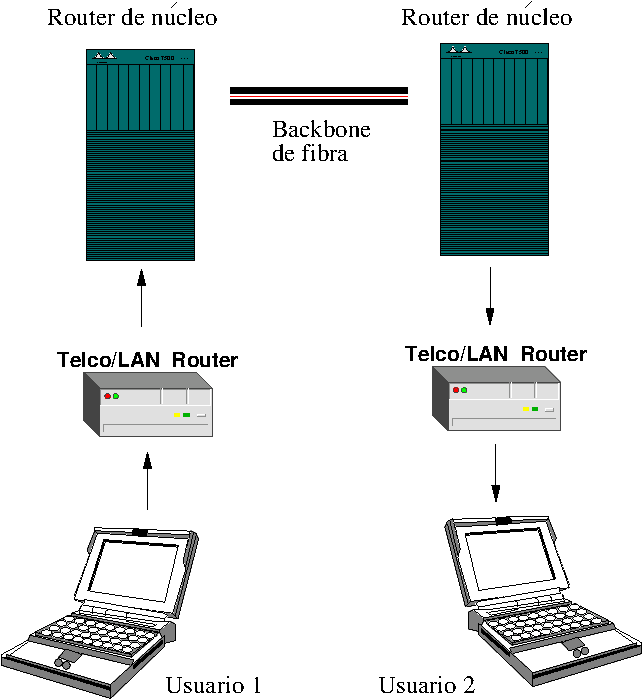
\includegraphics[width=4.0in]{graphs/internet.pdf}
    \caption{Simplificación del sistema de ruteo de Internet.}
    \label{arch:simp}
\end{figure}


Otro tipo de redes son las llamadas redes de difusión o \textit{broadcast}, que poseen algunas ventajas con respecto a las redes de conmutación de paquetes, tales como un sistema de ruteo mucho más simple que puede ser totalmente óptico, pero también tienen desventajas, tales como la necesidad de compartir el ancho de banda y problemas de seguridad inherentes al enviar la información a todos los nodos de la red. De esto se desprende que las redes de difusión deben generalmente contar con algún mecanismo que ofrezca privacidad, o de lo contrario su uso se restringe a aplicaciones que, o bien no requieren de ningún tipo de privacidad, o la privacidad se logra utilizando protocolos de alto nivel. Es sobre este tipo de redes donde se centra el aporte de esta Tesis.

Las redes de difusión no están limitadas al medio óptico. Pueden utilizar el medio electromagnético (por ejemplo, ondas de radio) o acústico (modems). Las comunicaciones de radio, por ejemplo, pueden ser espiadas por cualquier atacante que tenga una simple antena. Fue este problema en las comunicaciones de radio que impulsó la invención de técnicas criptográficas avanzadas en la segunda guerra mundial. Las comunicaciones de tipo difusión resultaron ser ideales para coordinar acciones bélicas en la segunda guerra, donde un emisor central podía impartir órdenes a toda el ejército utilizando ondas de radio, con la condicion obvia que únicamente aliados puedan participar de las comunicaciones. Esto motivó el desarrollo de los primeros dispositivos criptográficos tales como la máquina de Enigma \cite{kozaczuk1984enigma}, así como los primeros ataques matemáticos a la criptografía \cite{welchman1982hut}.

En tiempos modernos, las comunicaciones de tipo difusión fueron en gran parte desplazadas con respecto a las redes de conmutación de paquetes, especialmente en redes digitales de comunicaciones tales como Internet. Sin embargo existen nichos donde por motivos prácticos siguen siendo utilizadas redes de difusión casi exclusivamente, tal como la televisión y telefonía satelital. Gran parte de la complejidad de estos sistemas se debe a los sistemas de seguridad que deben contener para prevenir fraudes y pérdida de privacidad \cite{hanas1981addressable}.

Continuando con esta línea de investigación, los problemas de seguridad en las redes de difusión motivaron el diseño que utiliza un medio óptico o acústico donde la privacidad esté implementada en la capa física, sin requerir ningún tipo de soporte de software o del sistema operativo. El objetivo es crear una VLAN \textit{(Virtual Local Area Network, red local virtual)} donde cada cliente pueda realizar comunicaciones de datos privadas con cualquier otro, sin revelar ninguna información a los demás.

Esto apunta a fomentar el desarrollo de sistemas economicos de FTTH (\textit{Fiber to the Home}) sobre redes PON (\textit{Passive Optical Network}) \cite{lee2006fiber} donde un diseño de red de difusión óptica con seguridad a nivel físico permitiría utilizar componentes pasivos de muy bajo costo (ver Fig. \ref{arch:ftth}). Si bién es sencillo realizar un enlace punto-a-punto óptico o acústico utilizando cualquier algoritmo de encriptación simétrica estandard, la creación de una verdadera red, con múltiples clientes y canales punto-a-multipunto no tiene una solución clara hasta el momento.

Luego de un período de exploración de posibles diseños y soluciones se desarrolló un sistema de comunicaciones. Se calculó su eficiencia teóricamente y por medio de simulaciones, para finalmente proceder a su implementación como prototipo, primero sobre un medio acústico y finalmente sobre un medio óptico. 
En el medio acústico se utilizaron dispositivos informáticos comunes, tales como laptops y teléfonos celulares del tipo smartphone, utilizando los mismos micrófonos y parlantes de los mismos para establecer una red VLAN acústica. 
Para la implementación sobre medio óptico se utilizó una placa de desarrollo FPGA, un dispositivo capaz de procesar las altas tasas de transferencia del medio óptico.
Esta Tesis documenta las experiencias obtenidas en el diseño, implementación y medición del algoritmo implementado sobre varios dispositivos y medios diferentes.

\begin{figure}[!t]
  \centering
    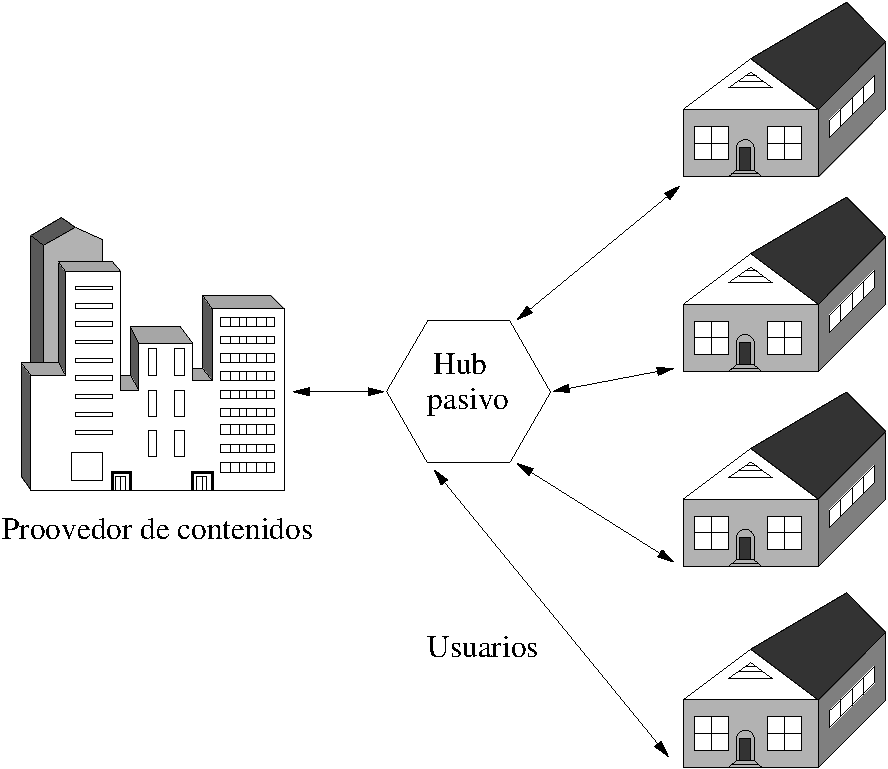
\includegraphics[width=3.5in]{graphs/ftth.pdf}
    \caption{Sistema FTTH propuesto. Un proovedor de contenidos (Ej. Datos, TV, o telefonía, lo que se denomina ``triple-play'') utiliza un concentrador de muy bajo costo para conectarse directamente a los usuarios finales por medio de una conexión de fibra óptica.}
    \label{arch:ftth}
\end{figure}

\section{Contribuciones}

A continuación citaremos las contribuciones que esta Tesis ha realizado a la comunidad, en la forma de artículos o patentes:

\textbf{Altas velocidades de transferencia en fibra óptica utilizando FPGAs de bajo costo. } \textit{A. A. Ortega, V. A. Bettachini, D.F. Grosz, J. I. Alvarez-Hamelin - Congreso de Microelectrónica Aplicada 2010 BsAs}: En este artículo se documenta una técnica para utilizar FPGAs (\textit{Field Programmable Gate Array}) con transceptores ópticos normales, a mayor velocidad que la documentada. Utilizando los circuitos internos del transceptor independientes de los circuitos de la FPGA que lo contiene, es posible generar señales de pruebas de hasta 12 Gbps, con una longitud máxima de patrón de 11 bits individualmente controlables. Estos patrones de prueba tienen aplicaciones tanto para la caracterización de canales como para la experimentación con pulsos Laser o eléctricos.

\

\textbf{ Point-to-point and Point-to-multipoint CDMA Access Network with Enhanced Security} \textit{ A. A. Ortega, V. A. Bettachini, J. I. Alvarez-Hamelin,  D.F. Grosz, Advanced Photonics 2011 Congress - Access Networks and In-house CommunicationsAccess Networks and In-house Communications, OSA Technical Digest, Optical Society of America}: Se presenta la primera versión de la red segura, funcionando sobre un medio de fibra óptica y con un aprovechamiento del medio del 13\%. Se propone una diseño de red segura en la capa física, utilizando la tecnica de time-hopping CDMA, y logrando comunicaciones criptográficamente seguras punto-a-punto y punto-a-multipunto. Una implementación con topología es en estrella es analizada, capáz de soportar hasta 128 usuarios situados hasta a 20 Km de distancia del nodo central. Se utiliza el algoritmo LDPC (\textit{(Low Density Parity Check)}) como parte del sistema de corrección de errores. Se demuestra la feasibilidad del sistema mediante simulaciones numéricas.

\

\textbf{Hamming-weight minimisation coding for CDMA optical access networks with enhanced security} \textit{ A. A. Ortega, V. A. Bettachini, J. I. Alvarez-Hamelin, D.F. Grosz, Future Generation Communication Technology (FGCT), 2012}: Este artículo se muestra un diseño similar al anterior, pero con una modificación en la pila de corrección de errores que eleva el aprovechamiento del medio al 33\%. Esto se logra eliminando la etapa de corrección LDPC y reemplazándola por una corrección de errores realizada directamente en el Bloom Filter encriptado, que es optimizado por el algoritmo de minimización de peso de Hamming. Utilizando un diseño en estrella, el sistema continua soportando 128 usuarios simultaneos situados hasta a 20 km de distancia del nodo central. Hay que destacar que estas características se cumplen utilizando un hub central pasivo. Utilizando un repetidor o hub central activo, las distancias pueden ser mayores.


\

\textbf{Encrypted CDMA Audio Network.} \textit{ A. A. Ortega, V. A. Bettachini, P. I. Fierens, y J. I. Alvarez-Hamelin.  Journal of Information Security - 2014}: Este artículo se centra en la implementación del protocolo sobre el medio acústico, ahondando en la sincronización, implementación y mediciones sobre distintos dispositivos móbiles, tales como celulares y laptops, demostrando que si bien la modulación necesaria para la creación de un canal Z tiene muy baja eficiencia espectral, es altamente compatible, resistente a interferencias y puede ser utilizada para transmitir de manera privada a distancias prácticas por la mayoría de los dispositivos testeados.


%\section{Patentes}

Se presentaron los siguientes pedidos de patentes en oficinas de patentes nacionales (Argentina) (patente asignada) e internacionales (EU) (patente en trámite al momento de escritura de esta Tesis):

\textbf{DISPOSITIVO Y MÉTODO PARA TRANSMISIÓN SEGURA DE DATOS SOBRE CANALES Z MEDIANTE CDMA (AR084155B1)}\textit{José Ignacio ALVAREZ HAMELIN, Victor Alexis BETTACHINI, and Alfredo ORTEGA. PCT, 12 2012. (Asignada)}

\textbf{Device and Method for the Secure Transmission of Data over Z-Channels Using CDMA (P11104EPPC)}\textit{José Ignacio ALVAREZ HAMELIN, Victor Alexis BETTACHINI, and Alfredo ORTEGA. EPO, Julio 2014. (En trámite)}


%\section{Contribución}


\section{Organización de este documento}

En el primer capítulo ``Introducción'' se presentan las motivaciones, contribuciones y algunas definiciones. Se describe en alto nivel la estructura de la Tesis.

En el segundo capítulo ``Fundamentos y Estado del arte'' se presenta un resumen de todas las tecnologías utilizadas, así como las definiciones necesarias.

El tercer capítulo ``Sistema propuesto: teoría y simulaciones'' se discuten las decisiones de diseño y se simula de manera numérica el sistema completo.

El cuarto capítulo ``Resultados experimentales: medios de transmisión óptica y acústica'' describe los detalles de implementación y mediciones en medios ópticos y acústicos. Se detalla el diseño de alto nivel de los generadores de trama en una FPGA para el protocolo en el medio óptico y la implementación en software que precisan los dispositivos móviles que utilizarán el medio acústico. Se detallan, también, los algoritmos de sincronización desarrollados, necesarios para las mediciones y para la creación de un prototipo funcional.

Finalmente, en el quinto capítulo, ``Conclusiones'', se finaliza la Tesis presentando las conclusiones obtenidas fruto de la investigación e implementación de los algoritmos y sistemas propuestos, y se sugieren posibles mejoras o aportes específicos a realizar en el futuro.

\chapter{Estado del arte}

\subsection{Códigos correctores de errores}
En toda comunicación es importante la confiabilidad de la misma, y como ningún sistema es perfecto es esperable que se produzcan errores en la transmisión que se presentan como bits erroneos detectados por el receptor. 

La idea de un código corrector de errores esta relacionada con la técnica de espectro expandido, siendo ambos métodos que ayudan a la transmisión de la información reduciendo la entropía de la información transmitida, o lo que es lo mismo, aumentando la redundancia de la información. 

La manera mas simple de corregir estos errores es usar un algoritmo de detección de errores como puede ser un Checksum, CRC o hash[CITA], e iniciar un proceso de retransmisión de la porción o trama de datos afectada. Esto posee la desventaja de ser costoso tanto en ancho de banda perdido, como en delay de transmisión. En enlaces de muy alta velocidad las elevadas tasas de retransmisiones hacen a este algoritmo sumamente ineficiente. 
Por lo que es deseable utilizar un algoritmo que pueda detectar y corregir errores basado solamente en los bits recibidos, sin utilizar retransmisiones. Esto se denomina Forward Error Correction Codes, o FEC Codes [CITA] de los cuales existen diferentes tipos de acuerdo con sus aplicación, performance y parámetros.

\subsubsection{BCH/Reed Solomon}
Los códigos BCH y Reed-Solomon son usados ampliamente en multitud de industria ya que son computacionalmente sencillos de implementar y muy eficientes desde el punto de vista de errores corregidos por bit agregado. Se basan en operaciones sobre grupos algebráicos cíclicos cuyas operaciones sobre sus símbolos dan como resultado otro símbolo válido dentro del grupo. 
Este tipo de código si bien es relativamente antiguo, es todavía utilizado en estándares de Ethernet de 10Gbps, 100Gbps y hasta 400Gbps [CITA: IEEE P802.3bj  o ``FORWARD ERROR CORRECTION FOR 400G: INITIAL THOUGHTS''] debido a su robustez, bajo over

\subsubsection{LDPC}
El esquema de corrección de errores LDPC (Low Density Parity Check) es muy utilizado actualmente debido a su gran capacidad de corrección de errores, en algunos casos muy cercana a la máxima capacidad teórica del canal.
Antes de ahondar en la descripción de este algoritmo cabe aclarar que a pesar de ser utilizado para ciertos modelos durante la primera fase de la investigación, fue descartado en la versión final por un modelo mas simple y con menos requerimientos de hardware que presenta una performance similar desde el punto de vista de corrección de errores.
Básicamente es un código lineal que utiliza una matriz de paridad grande y dispersa.
La matriz H es tal que cualquier codeword valido x cumple con $H*x=0$

\paragraph{LDPC: Generador de matriz}
La matriz generadora puede crearse facilmente si H es de la forma $[D|I]$, simplemente formando la matriz:
$$G=[I|D']$$
Donde D' es la transpuesta de la matriz D
Para la generacion de la matriz se opto por utilizar un algoritmo random y luego aplicando algunos tests, para lograr una matriz sistemática de rate entero (1/2, 1/3, etc.)
Para verificar se G genera vectores cuya matriz de paridad es H, puede verificarse que:
$$ H*G'=0 $$

Podemos definir la matriz de paridad H como una matriz de paridad que tenga mas de 3 unos por fila y una cantidad similar por columna. Buenos resultados se obtienen a partir de matrices de 200x100.
Se puede comenzar por una matriz vacía $H = 0$ del tamaño deseado, y ir agregándole unos al azar. Cierto análisis es necesario para garantizar que no se cumplan ciclos y que la cantidad de unos por columna y por fila es la deseada. De esto se encargan los algoritmos llamados evencol y evenrow.

El generador puede generar matrices de cualquier tamaño, de esta manera:

$$ ./genMatrix <width> <height> <ones per row>$$

La matriz se genera en la salida estandard. El formato es el utilizado por la libreria boost:ublas.

NOTA: La matriz siempre esta compuesta de simbolos en GF(2) (O sea, ceros y unos)

\paragraph{LDPC: encoder}

El vector inicial se toma de la entrada estandard y el codeword se emite en la salida estandard. La sintaxis es muy sencilla:

$$ ./ldpcen <matriz> < in >out $$
\paragraph{LDPC: decoder}
Si se invoca este filtro mediante el nombre decodificador, tomara el codeword de la entrada estandard, aplicara el algoritmo de belief-propagation (Hard-decision) y se emite el vector original por la salida estandard:
La diferencia radica que en nuestro caso, al ser un canal asimetrico no se permite el bit-flip de un valor cero a un valor uno, ya que es imposible que se produzca ese error.
La linea de comando es la siguiente:

$$ ./ldpcdec <matriz> <in >out $$

La conversion codeword->vector es sencilla, ya que al ser un codigo sistemático solo se necesita eliminar la parte del vector que representa la paridad añadida.

Se generaron muchas matrices, desde 256x128 hasta matrices muy grandes de 10000x5000, pero el tiempo de decodificacion crece enormemente para matrices grandes.

\paragraph{LDPC: optimizacion}

Debido a la naturaleza iterativa del decodificador ldpc, pronto se convirtio en el cuello de botella de la simulacion. Para acelerar el sistema, se opto por realizar la siguiente optimizacion:
LDPC consta basicamente de varios loops, dentro de los cuales se accede a la matriz de paridad, y a otras matrices que acumulan datos intermedios. Primeramente la implementacion fue realizada como mencionamos utilizando boost:ublas, pero luego se comprobo que una implementacion utilizando arrays de C era hasta 3 veces mas rapida.
Luego se procedio a realizar un algoritmo de ``unrolling'' de estos loops, generando codigo especifico a una matriz dada, sin ningun tipo de loop. Obviamente este codigo es mucho mas grande, pero la aceleracion provista es aun mayor, del orden de 8 veces mas rapido que en implementaciones iniciales.
La manera de invocar el generador de codigo es la siguiente:

$$ ./genLdpcDecoder matriz  > decodeGen.h $$

El archivo generado decodeGen.h es el decodificador especifico para la matriz dada. Este header de C es luego incluido desde el decodificador ldpcenc.cpp y compilado. Al ser generalmente un archivo de un megabyte para una matriz pequeña de 1024x512, el proceso de compilacion el largo y requiere de mucha memoria.
Por otra parte, no se optimizo el proceso de codificacion ldpc, ya que consiste solo de una multiplicacion de un vector por una matriz, y es una de las tareas en la que boost:ublas es especialmente eficiente.


\subsubsection{Viterbi/Convolucional}

\subsection{Espectro ensanchado}
\label{espectroensanchado}
El espectro ensanchado, Spread Spectrum o CDMA es una técnica donde se utiliza mucho mas espectro del medio de transmisión que el necesario para la transmisión correcta de los datos.
Los origines datan del 1900, cuando Nicola Tesla patentó el concepto de \textit{"Frequency hopping"}.
El spreading de la señal tiene varias ventajas:
\begin{enumerate} 
\item Resistencia al espionaje, ya que solamente las partes que conocen la señal de spreading pueden decodificar la señal original
\item Resistencia contra interferencias de banda angosta (No a interferencias de banda ancha como el ruido térmico)
\item Capacidad de acceso múltiple. Varios usuario pueden transmitir en la misma frecuencia mientras utilicen diferentes códigos.
\end{enumerate} 
Adicionalmente, al guiarse la señal expandida con un generador pseudo-aleatorio o PRBS, se puede agregar privacidad a la comunicación haciendo imposible decodificar los datos sin tener los parámetros del PRBS.

A su vez, se puede expandir la señal en tres dominios:
\begin{enumerate} 
\item Direct Sequence (CDMA): Se expande la señal multiplicándola (XOR) con la señal de spreading, generalmente mucho más rápida. Este método es el utilizado en WiFi y WiMAX, redes 3G de celulares, etc.
\item Frecuency Hopping: La señal de spreading es utilizada para variar la frecuencia portadora de la señal original. Este método es utilizado por ejemplo en BlueTooth. (Se utiliza Adaptive Frequency Hopping, un método para evitar frecuencias con mucha interferencia)
\item Time Hopping: La señal de datos no transmite todo el tiempo, sino que sufre de un delay que depende de la señal de spreading. Este método no es muy utilizado aunque lo estudiaremos detenidamente en nuestro caso ya que es muy sencillo de implementar con los recursos de los que disponemos.
\end{enumerate} 


La desventaja de la técnica del espectro expandido, que es utilizar mucho espectro por bits transmitido, o lo que también se denomina baja densidad espectral, a veces no afecta demasiado al tener el canal una cantidad disponible de espectro mucho mayor a la utilizada. Un ejemplo de un protocolo de comunicaciones que utiliza CDMA es el protocolo WIFI, en todas sus versiones, que utiliza un codigo DSS (Direct-sequence spread spectrum) para compartir una misma frecuencia entre varios nodos.

\subsection{Códigos de generación pseudo-aleatorio}
\label{PRNGs} 
Para que un código CDMA pueda utilizarse para obtener privacidad en la comunicación, es necesario que el parámetro a expandir, sea la frecuencia, el tiempo o el código utilizado, sea guiado o seleccionado por un generado pseudo-aleatorio o PRBS, que son algoritmos que basados en un parámetro de inicialización o semilla, son capaces de generar un stream de numeros aparentemente aleatorios, pero en realidad totalmente determinísticos. 
Es necesario que los nodos que participen de la comunicación puedan generar exactamente la misma secuencia y compartan el parámetro de generación o semilla. Esto es equivalente a lo que en criptografía se denomina un algoritmo criptográfico simétrico.
Existen muchas maneras y algoritmos de generar streams pseudo-aleatorios. Algunos algoritmos están optimizados para que su periodo (la cantidad de números en su salida antes que el patrón se repita) sea enorme, como por ejemplo el algoritmo Mersenne-twister.
Otro parámetro deseable en un PRBS es su sencillez y rapidez. Un generadores PRBS muy popular se denomina Lineal Congruential Generator y solo precisa de dos operaciones, una multiplicación y una suma.

Estos ejemplos carecen de una característica fundamental requerida en nuestro sistema: Que no se puedan predecir. Esta simple característica no es en realidad trivial ya que muchas técnicas existen para inferir datos acerca del generador PRBS, lo que supondría una falla en la seguridad de un sistema basado en dicho generador. Para evitar estos problemas existen los llamados generadores PRBS criptográficamente seguros. Como ejemplo podemos nombrar a los generadores shrinking o self-shrinking.
Constantemente surgen nuevos ataque a generadores ampliamente utilizados, tales como RC4~\cite{vaudenay2007passive}, por lo que es imprescindible estar actualizado en los avances de investigación criptográfica para diseñar un sistema seguro.


\subsection{Seguridad}
\label{Seguridad}
La propuesta es utilizar un sistema de espectro expandido con el objetivo principal de lograr la privacidad del canal al nivel físico.
Se fijaron los siguientes parámetros de seguridad:

. El sistema debe proveer confidencialidad, integridad y autenticidad de los datos.
. El sistema debe ser seguro sin importar la cantidad de clientes existentes o los datos que transmiten
. Un atacante no debe poder identificar los datos de un cliente, aunque controle todos los demas nodos de la red.

Con estos parámetros se busco el algoritmo CDMA adecuado. Las características de un sistema óptico hacen muy complejo el hardware requerido para lograr CDMA o Frequency-Hopping, pero implementar Time-hopping no presenta costo ni dificultad adicional, asi que este fue el seleccionado para la implementación de seguridad.
Varios algoritmos de asignación del time-slot fueron analizados. Se necesita que la salida de los mismos sean códigos ortogonales, o sea, deben poseer un generador capaz de crear streams pseudo-aleatorios que nunca coincidan para no generar colisiones entre los clientes. Esto no es trivial sin compartir algún tipo de información entre todos los clientes, lo que debilita la seguridad del sistema. Por ejemplo, códigos existentes llamados gold-codes permiten la generación de múltiples secuencias con baja cross-correlacion, muy util para coordinar dispositivos que comparten el medio. Pero desde el punto de vista de la seguridad, este código es trivialmente derrotado. Por ejemplo en un esquema donde un atacante controla todos los canales menos uno, el atacante podría simplemente dejar de transmitir y revelar la secuencia utilizada por la víctima, que forzosamente estara utilizando el canal restante.

Se decidió utilizar una codificación trivial: Seleccionar el time-slot de acuerdo a una secuencia criptográficamente segura estandard, totalmente independiente de los otros nodos. Es demostrable que esta decisión produce un sistema extremadamente simple y seguro. Como contrapartida, produce una cantidad muy elevada de colisiones que aumenta exponencialmente con el numero de clientes. Sin embargo, estas colisiones pueden ser corregidas mediante codificación adicional, y se logro una utilización de canal muy cercana al máximo teórico como se demostrara en la próxima sección. De echo, es en esta codificación adicional donde reside el principal aporte de esta tesis.

\subsubsection{Consideraciones de seguridad y fuerza de cifrado}\label{Seguridad-fuerza}
%% extraido de dline-pub.tex
Existen varios aspectos de seguridad en un canal de comunicaciones: Autenticación, confiabilidad, confidencialidad e integridad.
El esquema presentado en esta tesis utiliza la técnica de CDMA para proveer confidencialidad, confiabilidad e integridad entre dos o mas partes, y es equivalente a un esquema de clave simétrica donde la clave compartida es utilizada para inicializar el PRNG. Aspectos adicionales tales como la autenticación puede ser implementados luego utilizando protocolos de alto nivel.
El sistema propuesto fue específicamente diseñado tomando en consideración los ataques del tipo mencionados en Ref. \cite{Shake:05}.
Como la seguridad del sistema es dependiente de su algoritmo de PRNG, se debe poner especial cuidado en la selección e implementación del mismo, que debe ser un algoritmo generador de números aleatorios para usos en criptografía, o sea criptograficamente seguro. Existen muchos algoritmos que cumplen con estas necesidades, y el PRNG propuesto en esta tesis es el llamado self-shrinking generator~\cite{Meier:94}, pero puede utilizarse cualquier otro e incluso usar diferentes algoritmos para cada cliente, con la condición que dos clientes que deseen comunicarse deben utilizar el mismo algoritmo con los mismos parámetros y claves.
Como es en el caso de otros algoritmos de clave simétrica, la clave secreta debe distribuirse de ante mano utilizando un canal seguro.

Existe una vulnerabilidad adicional inherente a sistemas ópticos dispuestos como una red en estrella: Los algoritmos de CDMA dependen en la interferencia para ofrecer confidencialidad. Sin embargo, en un sistema óptico con topología en estrella hay lugares donde poca o ninguna interferencia es presente, por ejemplo, inmediatamente a la salida de un transmisor, donde la señal de salida es alta y puede medirse y discriminarse con respecto al ruido de las demas transmisiones facilmente.
Sin embargo, los símbolos productos de la minimización del peso de hamming fueron normalizados con respecto a un dígito normal, por lo que aún si un atacante pudier escuchar y discriminar cada uno de los bits de salida, no podría decodificarlos ni inferir información alguna acerca de los bits transmitidos.

Como distintos clientes emitiend odentro de una trama se puede superponer, el atacante observara un símbolo con un HW entre 1 y W$\times$K, pero no es posible reconstruir el orden correcto de los bits sin la semilla del algoritmo generador de PRNG.

Asi mismo, muchos algoritmos de cifrado se basan en la operación de XOR (El caso del algoritmo RC4), o bien una combinación de sustituir/mezclar los datos antes de la transmision (El caso de algoritmos AES y DES), o transformaciones mas complejas (Caso RSA o algoritmos de curvas elípticas), ver Ref.~\cite{Menezes:1996:HAC:548089}.
Sin embargo, todas estas técnicas necesariamente modifican el peso de Hamming de cada símbolo en una manera que no es óptima para el esquema propuesto combinado de CDMA/Bloom-filters ya que incrementa la interferencia inter-símbolo.
Como el algoritmo propuesto se basa en CDMA del tipo time-hopping, efectivamente encripta los símbolos de entrada mientras que mantiene el deseable bajo peso de Hammings en los datos de salida, lo que se refleja menor error y en una mayor utilización del ancho de banda disponible como se muestra en la Fig.~\ref{fig_use}.

\begin{figure}[t]
  \centering
  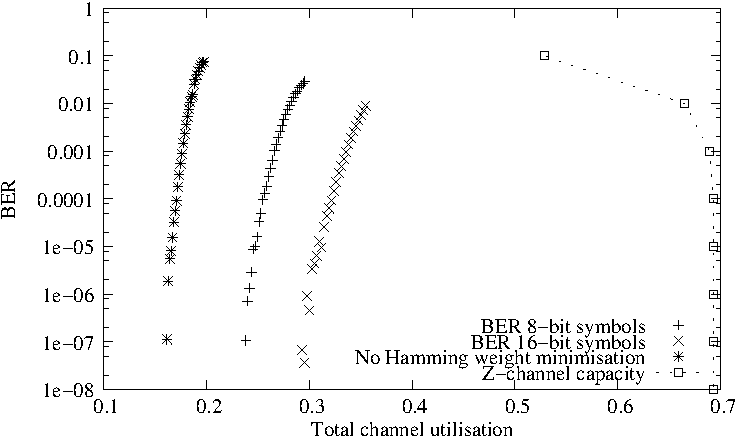
\includegraphics[width=0.48 \textwidth]{BERvsChannel} 
  \caption{Utilizacion del canal de 10 Gbps. Cada uno de los clientes (variando de 123 a 158) transmitieron 1 Gbit de datos. Notar la mejora en la utilización del ancho de banda comparada con~\cite{ortega11}.}
  \label{fig_use}
\end{figure}

En contraste con TDMA, en el esquema propuesto el atacante necesita interceptar cada una de las fibras ópticas para identificar cada usuario ya que son anonimizados luego de pasar por el hub central. Aun si el atacante puede identificar los datos, no podrá desencriptarlos sin poseer la clave correcta al estar los datos desordenados por el time-hopping y normalizado el peso de Hamming.

\chapter{Sistema propuesto: teoría y simulaciones}

\begin{figure}[t]
\centering
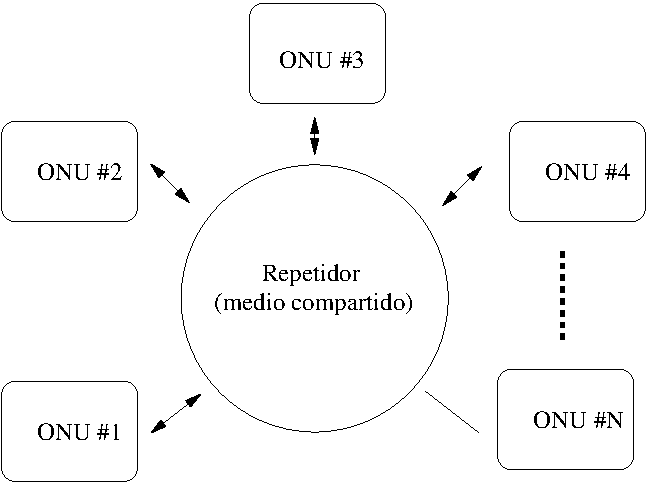
\includegraphics[width=4in]{graphs/hub}
\caption{Estructura de alto nivel del sistema propuesto, donde un repetidor central distribuye el tráfico a múltiples \textit{optical network units} (ONUs).}
\label{fig_hub}
\end{figure}

Se propone un sistema de comunicaciones punto a punto y punto a multipunto sobre medios compartidos, o también llamados medios de \textit{broadcast}. En la figura \ref{fig_hub} se detalla la estructura de alto nivel del sistema, que en la versión óptica (ver Fig. \ref{arch:fig1}) equivale a una red de tipo estrella con un concentrador/amplificador central. Utilizando diferentes medios de transmisión, esta configuración puede cambiar (por ejemplo, puede no ser necesaria la etapa de amplificación).
Al ser un sistema de tipo time hopping CDMA \ref{espectroensanchado}, cada cliente puede utilizar el medio por un intervalo determinado de tiempo denominado \textit{slot} o casillero. Esto permite utilizar el medio para múltiples clientes asignando a cada uno un casillero diferente. A diferencia de un sistema TDMA estándard, donde el casillero es asignado a cada cliente de manera periódica, en el sistema propuesto el casillero se asigna mediante un algoritmo CS-PRNG \ref{cap2:prng}. Esto tiene dos efectos fundamentales: 

\begin{itemize}
 \item Un atacante no puede predecir la posición en donde un cliente en particular transmite los datos. En particular, si el tamaño del casillero se reduce al mínimo de un solo bit, el atacante no puede inferir ninguna información acerca de los datos transmitidos sin conocer los parámetros del algoritmo CS-PRNG.
 \item Existirá una inevitable interferencia entre los clientes, lo que requiere la utilización de algoritmos de corrección de errores.
\end{itemize}

Como se describe en la sección \ref{cap2:prng}, existen varios algoritmos CS-PRNG estandarizados \cite{gallagherfips}. Esta Tesis no ahonda sobre el tema y nos limitaremos a indicar que puede seleccionarse cualquiera algoritmo utilizado por la industria que no posea ninguna vulnerabilidad conocida. Otra característica que debe maximizar el algoritmo seleccionado es la cantidad de bits pseudoaleatorios generados por ciclo de reloj, ya que al ser utilizados para seleccionar la posición de cada bit en una trama de largo $M$, se necesitarán generar como mínimo $\log_2(M)$ bits aleatorios por cada bit de datos\footnote{Esta cantidad es tal debido a para codificar una posición dentro de $M$ posibles valores, se necesitan $\log_2(M)$ bits.}, por lo que, en general, la velocidad del PRNG afectará directamente la velocidad total de codificación y decodificación del sistema.

Un aporte importante de esta Tesis es el desarrollo de un método de corrección de errores adaptados al medio de transmisión, aprovechando las características del canal para recuperar información con una elevada cantidad de interferencia, producida por el método aleatorio de selección de casillero de transmisión.

%Utilizando este Diseño físico con una etapa adicional de codificación y correccion de errores. El hub central es una etapa totalmente óptica que puede o no estar amplificada. Con la amplificacion optica se incrementa notablemente el rango, de 5 km a mas de 20 km.
La pila de codificación se detalla en la figura \ref{fig_comstack} donde puede verse su diseño convencional, excepto que en la última etapa de corrección de errores se aplica el algoritmo de filtros de Bloom, que aprovecha la característica de error asimétrico del canal Z para una corrección adicional.

\begin{figure}[t]
\centering
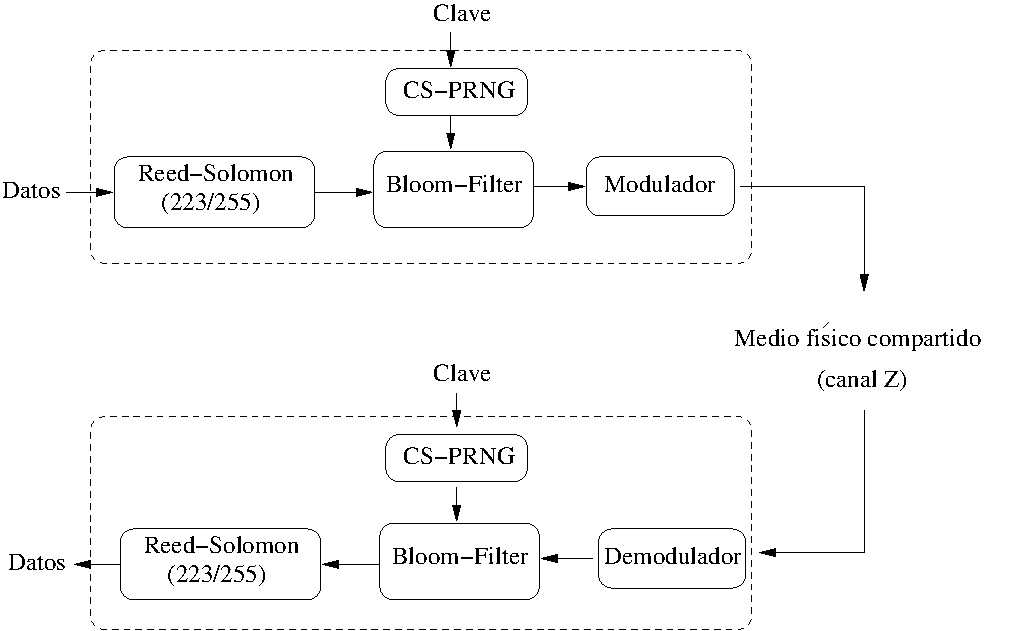
\includegraphics[width=5in]{graphs/Soft-stack3}
\caption{Diagrama esquemático del sistema de comunicaciones.}
\label{fig_comstack}
\end{figure}

\section{Códigos correctores de errores}

La selección del código corrector de errores debe ser guiada por los parámetros del sistema, teniendo en cuenta que al operar en enlaces con tasas de transmisión elevadas, una de las limitaciones más importantes es la velocidad de procesamiento de datos del sistema.

En nuestro caso, se utilizó una típica estructura de dos códigos de corrección, uno denominado código exterior (\textit{outer code}), y el segundo denominado código interior (\textit{inner code}).
La idea de utilizar dos códigos distintos es la de encadenar ambos algoritmos en serie para aprovechar las virtudes de dos tipos de corrección. Estos algoritmos se denominan códigos concatenados \cite{forney1966concatenated}. El motivo de utilizar códigos concatenados es que ciertos tipos de códigos tales como LDPC o códigos Turbo se caracterizan por poseer un piso de error elevado, que es un fenómeno donde el código pierde efectividad con relaciones señal/ruido elevadas \cite{richardson2003error}. Es para evitar esta pérdida de efectividad que se utiliza un segundo código corrector concatenado al primero, denominado código interior, que si bien no es tan efectivo con bajas relaciones de señal/ruido como el código exterior, es efectivo con señales de bajo ruido, haciendo que el sistema sea eficiente en cualquier condición.

Un parámetro importante en estos algoritmos es el retraso de codificación o latencia, es decir, la cantidad de tiempo (medida usualmente en ciclos de reloj del procesador) que demora un bit entrante a la etapa de corrección en ser procesado y salir de la misma, luego de la aplicación de la corrección de errores. Esta latencia es variable según el algoritmo. Algunos algoritmos con una latencia importante no son óptimos para utilizar en aplicaciones de bajo ancho de banda que precisan de retransmisiones o confirmaciones de los datos, ya que a cada confirmación debe sumarse también este retraso, y esto suele resultar en una disminución apreciable de la velocidad de las comunicaciones. A continuación se detalla el algoritmo de corrección seleccionado.

\subsection{Códigos de corrección Reed-Solomon}
Como código interior se seleccionó el algoritmo Reed-Solomon, un código de bloque con alta efectividad en relaciones de señal/ruido bajas. La cantidad de paridad agregada por el algoritmo, y por lo tanto, la potencia de corrección, puede ajustarse a cada aplicación, sin embargo, en computadoras digitales binarias suelen tener registros cuyo largo es múltiplo de 8 bits, por lo que es eficiente utilizar 8 bits como tamaño de símbolo en Reed-Solomon. Debido a esto, un código muy utilizado es aquel que posee un tamaño de bloque de 255 bytes y 223 bytes de datos, con 32 bytes de paridad. Estos parámetros logran que el código pueda detectar hasta 32 errores de byte y corregir hasta 16 errores dentro de los 223 bytes de datos del bloque \cite{wicker1999reed}. Al ser un estándar ampliamente utilizado, existen implementaciones eficientes de Reed-Solomon con estos parámetros específicos, tanto en software como en hardware.
Algunas desventajas de este algoritmo son:
\begin{enumerate}
 \item Elevado retraso de decodificación: Reed-Solomon es un algoritmo de complejidad temporal asimétrica. Esto significa que el retraso de codificación es mínimo (menos de 10 ciclos de reloj), pero el retraso de decodificación es elevado, pudiendo sobrepasar fácilmente los 1200 ciclos de reloj.
 \item Retraso inducido por buffer: si bien el retraso de decodificación es elevado y requiere un procesamiento no despreciable, el tiempo necesario para acumular un bloque de 256 bytes de datos en memoria para comenzar con la decodificación introduce un retraso importante, especialmente si el sistema se utiliza con bajo ancho de banda, tal como es el caso en la implementación acústica.
\end{enumerate}
 
Ambas desventajas se solucionan ajustando los parámetros de Reed-Solomon para utilizar un menor tamaño de bloque, o bien utilizando un algoritmo similar con menor tamaño de bloque, tal como BCH \cite{bose1960class}. Sin embargo, una biblioteca eficiente y disponible que permita el uso de BCH no pudo ser encontrada, por lo que la selección final fue el estándar Reed-Solomon (255, 223).

Para la simulación numérica por software se utilizó la biblioteca \textit{LibFEC} de Phil Karn~\cite{libfec}. Para la implementación en FPGA se utilizó la versión del algoritmo provista de manera gratuita en la biblioteca de núcleos de IP de Xilinx \cite{Xilinx:DS251}.

%Con posibilidad de error de simbolo P, la posibilidad de error de un codigo reed-solomon R(n/k) es:
%$$P_{rs}= \sum_{k=(\frac{n-k}{2}+1)}^{n} \binom{L}{i} * P^{i} * (1-P)^{L-i} $$
La implementación del algoritmo Reed-Solomon utilizada posee 32 bytes de paridad y 223 bytes de datos, lo que representa una adición de 14\% a la cantidad total de datos a transmitir. Este código permite corregir hasta 16 errores dentro del bloque, que pueden estar consecutivos, por lo que Reed-Solomon suele utilizarse en canales con errores de tipo \textit{``erasure''} o errores de ráfaga, donde los errores no están uniformemente distribuidos, sino que están agrupados temporal o espacialmente.

%En ciertas ona ventaja muy importante es que el codigo de correccion exterior puede facilmente detectar la presencia de un error aunque no pueda corregirlo. Esta informacion es una lista con las posiciones en las cuales se tiene la certeza que los símbolos fueron interferidos denominada lista de síndromes, y puede suministrarse al algoritmo de correccion de errores para que la capacidad de corrección del mismo puede aumentar hasta un 100\%~\cite{Moon:05}.

\subsection{Características de implementación}
Un parámetro importante en la selección del algoritmo es la facilidad de implementación sobre hardware digital. Ciertas características se vuelven importantes al pasar de implementaciones de software a hardware, tales como tamaño, memoria utilizada y velocidad máxima alcanzada con el hardware disponible, con el objetivo de que el sistema funcione a tasas de transferencia en el orden de gigabits por segundo.

A continuación, se listan las características de la implementación en hardware (FPGA) de Reed-Solomon:

El bloque de IP se denomina Reed-Solomon Encoder/Decoder 7.1 de LogiCORE IP. Con respecto al retraso, Reed-Solomon es un algoritmo de complejidad asimétrica, es decir, la complejidad espacio-temporal y ciclomática \cite{mccabe1976complexity} de los algoritmos de codificación de Reed-Solomon son diferentes a las de su correspondiente algoritmo de decodificación. En general, la decodificación es más costosa en términos de recursos de hardware y de latencia agregada al sistema. Según la especificación de esta implementación~\cite{Xilinx:DS252}, el decodificador Reed-Solomon con configuración CCSDS \cite{coding1999consultative} (que implementa el estándar (255,223)) posee un tamaño de 1364 LUTS (\textit{Look-up tables}, los elementos lógicos de la FPGA) y 3 bloques de RAM. Como comparación, el diseño completo presentado en esta tesis, posee un tamaño de aproximadamente 20000 LUTS, mientras que la FPGA utilizada posee una capacidad de 50000 LUTS. La velocidad máxima de reloj de este algoritmo en la FPGA utilizada es de aproximadamente 350 Mhz, superior a la velocidad requerida por el sistema completo a máxima velocidad, que es de aproximadamente 70 Mhz.
La cantidad de recursos utilizados por el codificador es menor: son necesarios sólo 300 LUTS y un bloque de memoria, aunque la velocidad máxima es similar~\cite{Xilinx:DS251}.

\subsection{Cálculo de latencia de la etapa de corrección de errores}
La latencia en un sistema se define como el tiempo que demora un bit en atravesarlo en su totalidad. Específicamente, el retraso en la etapa de corrección de errores representa un porcentaje importante de la latencia total en la pila de comunicación del sistema. La latencia de un algoritmo es específica a una implementación en particular.

La latencia total estará dada por el retraso introducido por la codificación sumado al retraso introducido por la decodificación, ya que los datos deben atravesar ambas etapas. Sin embargo, el tiempo de latencia en la etapa de codificación es despreciable (del orden de 5 ciclos de reloj~\cite{Xilinx:DS251}), por lo que se utilizarán sólo los valores de latencia de la etapa de decodificación. 

La latencia de la etapa de decodificación puede ser calculada de manera exacta mediante ecuaciones provistas por la hoja de datos \cite{Xilinx:DS252}. Se puede utilizar la figura \ref{fig_rslat} para obtener rápidamente el retraso de procesamiento. El parámetro $t$ se calcula como $t=(n-k)/2$ donde $n$ es la cantidad de símbolos totales en el bloque (en nuestro caso 255) y $k$ es la cantidad de símbolos de datos en el bloque (223 en nuestro caso) por lo que $t=16$.  El retraso total introducido por la decodificación estará dado por la latencia (en nuestro caso es aproximadamente 650 ciclos de reloj) sumado al retraso producto de cargar un bloque entero de datos en el decodificador. Como los datos deben ingresarse a la memoria del decodificador por medio de un bus serial de un byte de capacidad, se necesitan 255 ciclos adicionales por cada bloque. 

Sumando ambos valores, e ignorando la mínima latencia de codificación, podemos afirmar que la latencia introducida por el algoritmo Reed-Solomon en el sistema es de 900 ciclos.

\begin{figure}[t]
  \centering
  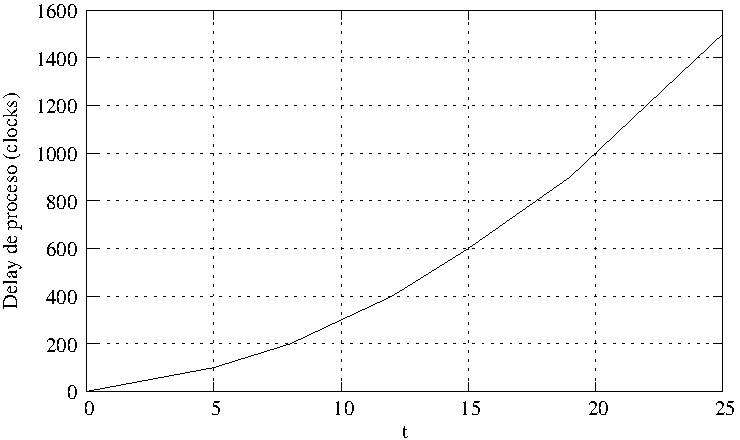
\includegraphics[width=0.8 \textwidth]{graphs/rsDelay.pdf} 
  \caption{Retraso de proceso de la implementación de Reed-Solomon utilizada~\cite{Xilinx:DS252}.}
  \label{fig_rslat}
\end{figure}


%\subsection{Optimizaciones propuestas}
% 
%Existen ciertas optimizaciones que podrían haberse realizado si se hubiera optado por implementar el algoritmo desde cero, pero que al utilizar una implementación pre-existente no se realizaron. Estas optimizaciones están relacionadas con la características del canal asimétrico, que presenta las ventajas de tener la certeza de que ciertos símbolos fueron transmitidos correctamente. Una posible optimización de Reed-Solomon para su utilización sobre canales Z se plantea para una trabajo futuro.

\section{Canal Z con filtros de Bloom}

En esta sección se describe el modelo del canal por el cual estamos transmitiendo datos, específicamente el modelo de ruido del mismo. 
Un canal de comunicaciones puede clasificarse primeramente según el tipo de información transmitida, sea binaria o analógica \cite{MacKay:2002}.
Una subclasificación del canal de comunicaciones puede realizarse según el comportamiento del ruido del mismo.

Las comunicaciones digitales suelen modelarse como un canal discreto sin memoria (\textit{discrete memoryless channel}), ya que poseen un alfabeto de símbolos de entrada $A_{x}$, que son los datos que se desea transmitir, y un alfabeto de símbolos de salida $A_{y}$ , que son los símbolos detectados por el receptor. El canal es discreto, ya que la cantidad de símbolos posible es finita. Se dice que el canal no posee memoria debido a que la probabilidad de obtener un símbolo de salida dado no depende de todos los símbolos de entrada, sino solamente del último símbolo enviado.

Otro parámetro importante que define a un canal discreto es la distribución de probabilidades condicionales $P(y|x)$ entre ambos alfabetos, es decir, la posibilidad de que al recibir el símbolo $x$ se haya transmitido el símbolo $y$. Esta distribución puede representarse como un diagrama de distribución de probabilidades (ver figura \ref{fig:canbin}) o una matriz.

De acuerdo con la distribución de probabilidades de error que mejor represente al canal físico de transmisión, el tipo de canal que mejor modela las transmisiones digitales por fibra óptica es el denominado canal Z (\textit{Z Channel}), un canal digital en el que el ruido afecta sólo uno de los símbolos binarios a transmitir.

Es este modelo de ruido nos permite innovar en el diseño de algoritmos, adaptándolos y optimizándolos para aprovechar la distribución de ruido, ya que la mayoría de los algoritmos de corrección de errores están pensados para un canal de ruido simétrico y generalmente analógico.
Empezaremos primeramente estudiando un modelo simplificado del canal por el cual vamos a trasmitir, el mencionado canal simétrico binario.

\section{Probabilidad de error del canal transmitiendo en un solo slot del frame}

\begin{figure}[t]
  \begin{center}
    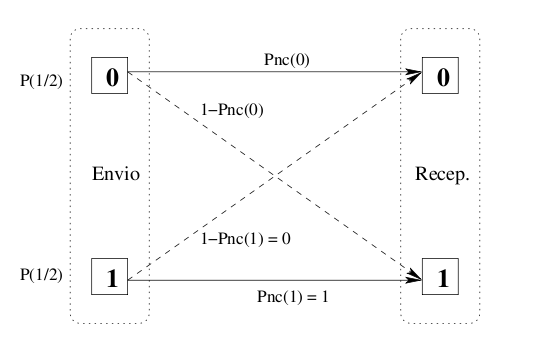
\includegraphics[scale=0.50]{graphs/canalBinario.png}
  \end{center}
\caption {Canal binario: esquema de probabilidad.}
\label{fig:canbin}
\end{figure}

Procederemos a calcular la probabilidad de no-colisión de un cliente.

Sea $M$ la cantidad de casilleros por trama y $n$ la cantidad de clientes o usuarios.

Entonces, la probabilidad de no colisión para un usuario en un slot dado es
\begin{equation}
P_{nc}=\left(\frac{M-1}{M}\right)^{n-1}
\end{equation}

Esta ecuación es válida bajo la hipótesis de que todos los clientes eligen el slot a transmitir de manera aleatoria, y de manera independiente. También consideramos que los usuarios utilizan sólo un slot.

Para simplificar, hablaremos de 'colisión' de símbolos cuando uno o más usuarios escriben en el mismo slot de un usuario y causan un error en el canal. De esta manera, en el canal Z, cuando se transmite un 1, las colisiones con símbolos transmitidos por otros usuarios no causan un error. Diremos, por tanto, que la probabilidad de no colisión de un 1 transmitido es 1, es decir, $P_{nc}(1) = 1$. Por otro lado, cuando se transmite un 0, sólo las colisiones con 1s transmitidos por otros usuarios generan error en el canal.

Siendo $P_{nc}(1)$ la probabilidad de no colisión del símbolo uno, y $P_{nc}(0)$ la probabilidad de no colisión del símbolo cero, la probabilidad total de no colisión para un usuario en un canal Z es

\begin{equation}
P_{nc}=P(1)\cdot P_{nc}(1) + P(0) \cdot P_{nc}(0) 
\end{equation}
Asumiendo que todos los usuarios transmiten un stream de datos aleatorio, tenemos que $P(1)=P(0)=\frac{1}{2}$. Entonces podemos desarrollar $P_{nc}$ como

\begin{eqnarray}
P_{nc} & = & \frac{1}{2} \cdot 1 +  \frac{1}{2} \cdot \sum_{i=0}^{n-1} 
C^{n-1}_{i} \left(\frac{M-1}{M}\right)^i  \left(\frac{1}{M}\right)^{n-1-i}  \left(\frac{1}{2}\right)^{n-1-i} 
\end{eqnarray}

La complejidad de la ecuación 3.2 se encuentra entonces en el desarrollo de $P_{nc}(0)$. Cada término de la sumatoria del segundo término del RHS de la ecuación 3.3 da la probabilidad de que $(n-i-1)$ usuarios escriban un 1 en el slot seleccionado.
El factor $C^{n-1}_{i}$ suma sobre todas las combinaciones posibles de canales que no hayan colisionado, que son hechos independientes.
\noindent Luego, $\left(\frac{M-1}{M}\right)^i$ es la probabilidad de no colisión de $i$ canales (se suma para todo posible número de canales no
colisionando: $1\leq i\leq n$, que están en otro casillero), $
\left(\frac{1}{M}\right)^{n-1-i}$ es la probabilidad de colisión de los restantes
$n-1-i$, y la colisión se produce cuando los otros canales
transmiten el símbolo $1$ cuya probabilidad es $\left(\frac{1}{2}\right)^{n-1-i}$.
%El factor combinatorio (C^{n-1}_{i}) me da la cantidad de grupos de i (o de n-1-i) usuarios de entre los (n-1) restantes puedo formar (es decir, la cantidad de formas que puedo escoger grupos de (n-1-i) personas que me sobreescriban mi querido 0).  El segundo factor me da la probabilidad de que i de los restantes (n-1) usuarios seleccionen OTROS slots. El tercer factor me da la probabilidad de que el grupo selecto de (n-1-i) usuarios elijan MI slot. Finalmente, el último factor me da la probabilidad de que los rhdp del grupo selecto de (n-1-i) usuarios escriban un 1 en MI slot



\noindent Teniendo en cuenta que $ \sum_{i=0}^{n-1}
C^{n-1}_{i} \left(\frac{M-1}{M}\right)^i  \left(\frac{1}{2M}\right)^{n-1-i}$ es la potencia $n-1$ de un binomio, reemplazando tenemos
\begin{eqnarray}
P_{nc} & = & \frac{1}{2} +  \frac{1}{2} \cdot \left(\frac{M-1}{M} + \frac{1}{2M} \right)^{n-1} \\
P_{nc} & = & \frac{1}{2} +  \frac{1}{2} \cdot \left(1- \frac{1}{2M} \right)^{n-1} \\
P_{nc} & \simeq & \frac{1}{2} +  \frac{1}{2} \cdot e^{\frac{-n}{2M}}
\end{eqnarray}

%\noindent donde la última aproximación vale para $n=M$ y $n > 2$.


Es decir, la probabilidad de no colisión depende de la relación $n/M$. Si $M>>n$, entonces $P_{nc}$ se aproxima a 1, que es una característica deseable en el sistema.
\iffalse

\vspace{5mm}

\noindent Para el caso de {\em Bloom} filters con $k$ filtros\footnote{Se envían $k$ repeticiones del bit en canales distintos, entonces basta que sólo uno de ellos sea 0 para que recibamos un 0 en un canal óptico.} la probabilidad de no colisión es:
\begin{eqnarray} 
P_{nc}^{k} & = &  P(1) \cdot P_{nc}^{k}(1) + P(0) \cdot P_{nc}^{k}(0)\\ \label{Pnc_k}
\end{eqnarray}
Sabiendo que la probabilidad de no colisión para el 0 es:
\begin{eqnarray}
P_{nc}^{k}(0) & = & 1 - \big(P_{c^k}(0)\big)^k 
\end{eqnarray}
Pero la probabilidad de colisión para el 0 cuando se transmiten $k$ copias es:
\begin{eqnarray}
P_{c^k}(0) & = & 1 - \big(P_{nc^k}(0)\big)  \enspace,
\end{eqnarray}
y que además la probabilidad de no colisión para los $k$ casilleros del Bloom
filter es
\begin{eqnarray}
P(\mbox{no col.} k) &=& P(\mbox{no col.}1)\cdot P(\mbox{no col.}2)\cdot P(\mbox{no col.}3)\cdots P(\mbox{no col.}k)\\
&=&\left(\frac{m-1}{m}\right)\cdot\left(\frac{m-2}{m-1}\right)\cdot\left(\frac{m-3}{m-2}\right)\cdots\left(\frac{m-k}{m-(k-1)}\right)\\
&=& \frac{m-k}{m} \enspace.
\end{eqnarray}
Luego la probabilidad de colisión con alguno de las $k$ copias del bit es
\begin{eqnarray}
P(\mbox{col.}k)&=& 1-P(\mbox{no col.} k)\\
&=& 1-\frac{m-k}{m}\\
&=& \frac{k}{m} \enspace.
\end{eqnarray}
Entonces reemplazamos y calculamos:
\begin{eqnarray}
P_{c^k}(0) & = & 1 - \left(\sum_{i=0}^{n-1} C^{n-1}_{i} \left(\frac{m-k}{m}\right)^i \left(\frac{k}{2m}\right)^{n-1-i} \right)  \\
& = &  1-\left( 1-\frac{k}{2m}\right)^{n-1}
\end{eqnarray}
Reemplazando esta ecuación en~\ref{Pnc_k} obtenemos:
\begin{eqnarray}
P_{nc}^k & = & \frac{1}{2} + \frac{1}{2} \left( 1- \left( 1- \left( 1- \frac{k}{2m} \right)^{n-1}  \right)^{k}  \right) 
\end{eqnarray}

Sin embargo, este calculo es incorrecto, comparandolo con los datos que da el simulador. La formula entrega valores de error menores con respecto a los reales, como se observa en la figura. 
Los trazos del mismo color corresponden a el mismo K con azul(K=1), verde (K=2) y rojo(K=4). M=256

\subsection{Entropía}

Comenzemos por lo básico:

Segun Shannon, el \textbf{contenido de informacion} h(x) de un suceso x dada la posibilidad que suceda P(x) es:
$$ h(x) = log_{2}\left(\frac{1}{P(x)}\right) $$

Y la entropia de un conjunto A, H(A) se define simplemente como el promedio del contenido de información:

$$ H(A) = \sum_{x E A_{x}} P(x)log_{2}\left(\frac{1}{P(x)}\right)$$

En un canal binario solo dos sucesos existen, uno con probabilidad p, y otro con probabilidad 1-p, por lo tanto para p siendo la probabilidad de error:

$$ H(p) = -p log_{2}(p)-(1-p)log_{2}(1-p) $$

\subsection{Entropia condicional}

Vamos a analizar la entropia de dos conjuntos X de entrada y Y de salida interrelacionados.

La entropia condicional de X dado $y=b_k$ donde $b_k$ es un valor dado, es la entropia de la distribucion de probabilidad $P(x|y=b_{k})$:
$$H(X|y=b_{k}) = \sum_{x \in A_{x}} P(x | y=b_{k})\log_2\left(\frac{1}{P(x | y=b_{k})}\right) $$

La entropia codicional de X dado Y es el promedio, sobre y, de la entropia condicional de X dado y:
$$H(X|Y) =  \sum_{xy \in A_{x}A_{y}} P(x,y)\log_2\left(\frac{1}{P(x,y)}\right) $$

\subsection{Información mútua}
La información mútua entre X e Y es:
$$I(X;Y) = H(X)-H(X|Y)$$
Mide el promedio de reduccion de la incertidumbre acerca de x que resulta de saber el valor de y, o viceversa: la cantidad promedio de informacion que x revela acerca de y.

\fi
\subsection{Capacidad de canal}

Existe una relación entre la probabilidad de error $Pb$ de un canal y la máxima velocidad de transmisión de datos posible en el mismo.
Esta relación fue estudiada por Claude Shannon en 1948 en un artículo pionero de la teoría de la información \cite{shannon48} y es conocida actualmente como teorema de Shannon-Hartley, también llamado teorema de codificación de canales con ruido (\textit{noisy channel coding theorem}).

La capacidad $C$ de un canal discreto sin memoria es la máxima información mutua entre los alfabetos $X$ de entrada e $Y$ de salida:

\begin{equation}
C = \max_{{\cal{P}}_x} I(X;Y) 
\end{equation}

Para hallar el máximo podemos derivar $I(X;Y)$ con respecto a la probabilidad $P_x$.
De \cite{MacKay:2002}, para un canal binario simétrico sin memoria con probabilidad de error $p$, la capacidad máxima $C$ es:

\begin{equation}\label{Cap}
C \approx 1 - H(p) 
\end{equation}

donde $H(p)$ es la función de entropía binaria

\begin{equation}\label{Hp}
 H(p) = [p \cdot log_2(p) + (1-p)\cdot log_2 (1-p)]
\end{equation}

Si expandimos $H(p)$ en \ref{Cap}:

$$ c = 1-\left(p \cdot \log_2\left(\frac{1}{p}\right) + (1-p) \cdot \log_2\left(\frac{1}{1-p}\right)\right) $$
Simplificada:
$$ c = 1 + p \cdot \log_2(p) + (1 - p) \cdot \log_2(1-p) $$

En la figura \ref{fig:CompBZ} puede verse la evolución de la capacidad del canal binario simétrico, que es máxima para $p=0$ y $p=1.0$, mientras que es cero para $p=0.5$, ya que con 0\% de probabilidad de error la capacidad es la máxima (no hay interferencia) y con 50\% de error la capacidad es cero y es imposible transmitir dato alguno. Quizás contra intuitivamente, con 100\% de posibilidad de error, la capacidad también es máxima, ya que equivale a invertir cada símbolo transmitido, operación que no introduce error alguno en los datos.

%Sin embargo esta capacidad es menor que la que realmente tenemos en nuestro canal, ya que un Z-channel se adecua mayormente a los medios de transmisión ópticos. Describiremos en detalle este caso especial en la siguiente sección. ??

\subsection{Canal Z}
\label{canalZ}
Un canal Z difiere de un canal binario, ya que las probabilidades de error de bit son asimétricas.
Los canales Z se usan generalmente para modelar sistemas de transmisión ópticos.

\begin{figure}[th]
  \begin{center}
    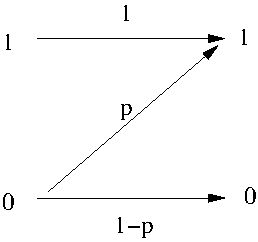
\includegraphics[scale=1]{graphs/zchannel}
  \end{center}
  \caption{Diagrama: canal Z. El diagrama superior podría representar un canal de fibra óptica donde un 1 representa el Laser encendido.}
  \label{fig:Gal}
\end{figure}

Para un canal Z, la distribución de probabilidades de la información mutua $I(X;Y)$ es diferente a la de un canal binario simétrico \cite{Tallini:02}, por lo que obtenemos un máximo diferente:

\begin{equation}\label{CapA}
C_{Z} \approx 1 - \left(\frac{1}{2}*H(p)\right)
\end{equation}

Por lo tanto, expandiendo $H(p)$ (definida en \ref{Hp}) en \ref{CapA}:

$$ C_{Z} = \log_2\left(1+(1-p) p^{p/(1-p)}\right) $$

La diferencia entre las capacidades de ambos tipos de canal puede apreciarse en la figura \ref{fig:CompBZ}. El mínimo de capacidad en el canal simétrico se da cuando $p=0.5$, mientras que en el canal asimétrico, el mínimo de capacidad se produce cuando $p=1.0$.

\begin{figure}[th]
  \begin{center}
    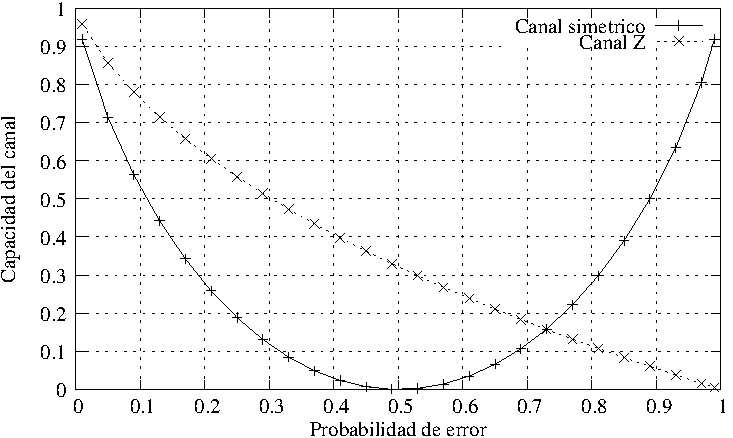
\includegraphics[scale=1.1]{graphs/grafico_comparacion_capacidad_binaria_z}
  \end{center}
  \caption{Capacidad de un canal binario simétrico con respecto a uno asimétrico o canal Z.}
  \label{fig:CompBZ}
\end{figure}


\section{Filtros de Bloom}
\label{Bloomf}
Como se discutió en la sección \ref{Seguridad} , la colisiones de símbolos son inherentes al tipo de codificación seleccionada.
En la modulación OOK (\textit{on-off keying}) utilizada en un medio óptico, sólo los ‘1’s transmitidos pueden interferir con ‘0’s. Este comportamiento puede ser modelado como un canal-Z porque la superposición de pulsos de luz individuales representando ‘1’s puede solamente ser identificados como un ‘1’s. De esto se desprende que un ‘0’ recibido es un signo inequívoco de la ausencia de pulsos en el casillero de tiempo leído.
Una buena estructura para representar este tipo de datos es el filtro de Bloom \cite{Bloom70space/timetrade-offs}, que se utiliza comúnmente como función de \textit{hash}~ \cite{song2005fast}. Dichas funciones constituyen una familia de algoritmos utilizados como tests eficientes (complejidad temporal $O(1)$) de pertenencia de un miembro en un conjunto, a diferencia de una búsqueda normal que puede tener una complejidad temporal mucho mayor (podemos citar el algoritmo de búsqueda binario, con una complejidad de $O(log_2(n))$.

La manera en que se implementó este algoritmo en el sistema propuesto se basa en copiar cada bit en $K$ casilleros de la trama transmitido, siendo la trama la representación física del filtro de Bloom.
En el extremo receptor es suficiente recibir un solo ‘0’ entre las $K$ copias del bit, para inferir que el bit original era originalmente un ‘0’, mientras que si el bit original era un ‘1’, las colisiones no tienen efecto debido a la naturaleza del canal-Z.

En la figura \ref{fig:Bloomf} puede apreciarse gráficamente como se utiliza un filtro de Bloom para la transmisión de 12 clientes con una repetición $K=3$. 

\begin{figure}[th]
  \begin{center}
    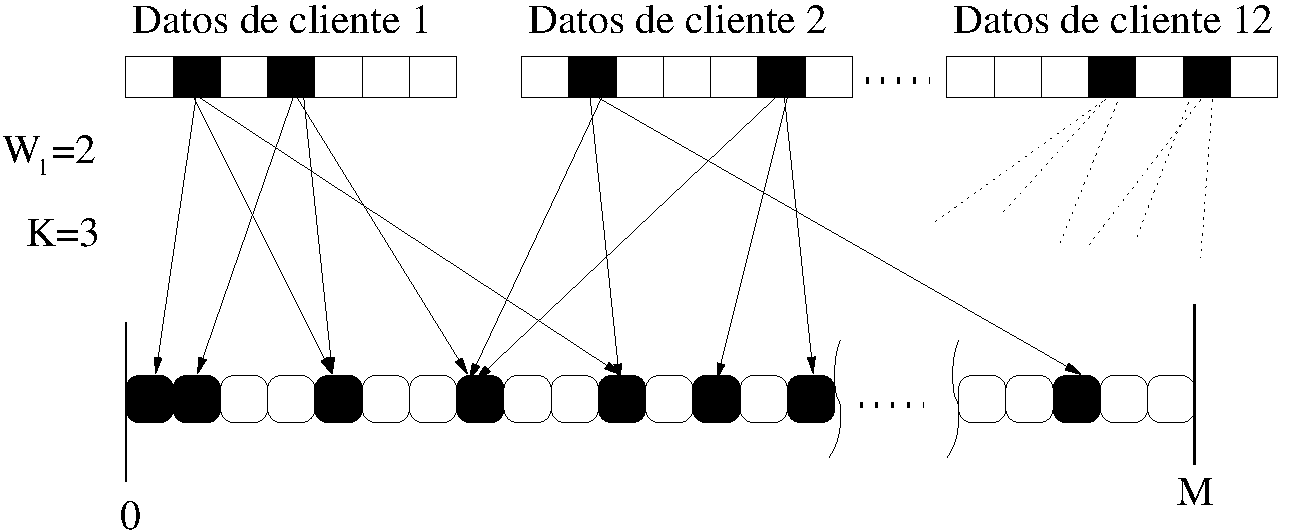
\includegraphics[scale=0.55]{graphs/frame-sp}
  \end{center}
  \caption{Filtro de Bloom. M es el largo de la trama. $W_1$ es el peso de Hamming mínimo. El parámetro K es el número de repeticiones.}
  \label{fig:Bloomf}
\end{figure}

%As discussed in section 2, this leads to collisions. Since the modulation format is OOK, only transmitted ‘1’s can interfere with ‘0’s.
%This behaviour can be modelled as a Z-channel because the superposition of individual light pulses representing ‘1’s
%can only be identified as a ‘1’, but a received ‘0’ is an unmistakable sign of the absence of pulses in a given time casillero.
%We found that the Bloom filter [2] provides a convenient structure to correct for errors in this type of channel. This
%technique is borrowed from hashing algorithms and is used to test whether an element is member of a given set. The
%way that we implement this algorithm relies on copying every bit in K casilleros of the transmitted frame. On the receiving
%end it is sufficient to receive a single ‘0’ out of K copies in order to correctly retrieve the original transmitted ‘0’,
%whereas collisions have no effect on ‘1’s.

\subsection{Filtros de Bloom encriptados}

En esta etapa se realiza la encriptación de los datos, reemplazando el algoritmo de hashing que selecciona las posiciones de los datos dentro del filtro de Bloom por una función pseudoaleatoria criptográficamente segura, de modo que los bits de datos de los diferentes clientes se posicionan aleatoriamente en la trama, y sólo es posible decodificar los datos si se tiene exactamente la misma secuencia pseudoaleatoria con que fueron posicionados originalmente. Como esta secuencia está determinada por la semilla del algoritmo PRNG, los participantes deberán compartir esta semilla previamente, que es el equivalente a una clave o password simétrico. 

Desde el punto de vista de la modulación, el algoritmo PRNG selecciona la posición temporal dentro de la trama, por lo que este esquema es equivalente a una transmisión time hopping, con la única salvedad de que el algoritmo de filtro de Bloom requiere $K$ repeticiones de los datos para poder recuperarlos de colisiones en la recepción.

Para poder decodificar los datos en el filtro de Bloom receptor es necesario que todos los participantes posean la misma secuencia pseudoaleatoria, es decir, la misma clave o semilla generadora \ref{PRNGs} del mismo PRNG utilizado para codificar los datos, y todos deben estar sincronizados a nivel de trama con el nodo originante. Las tramas del cliente originante y el receptor deben empezar y terminar al mismo tiempo para poder regenerar exactamente todas las posiciones en donde se transmitieron los datos. 

Sin embargo, los demás clientes que utilizan el medio compartido sólo causan interferencia y por lo tanto la sincronización a nivel de trama sólo es necesaria entre los clientes que deseen compartir el canal encriptado. Esto reduce los requerimientos de sincronización y simplifica la implementación de la red.

Finalmente, es deseable, pero no necesario, que todos los clientes mantengan una sincronización a nivel de bit, es decir, que los tiempos de transmisión de todos los clientes estén suficientemente alineados para que el casillero de un cliente sólo pueda superponerse con otro casillero de otro cliente y le cause un solo error de bit. Si esta sincronización no se mantiene, un casillero podría interferir con dos casilleros de otro cliente que está desalineado con respecto al primero, provocando dos errores en lugar de uno solo y aumentando los requerimientos de corrección de errores en el sistema.

\section{Minimización de peso de Hamming}
%% extraido de dline-pub.text
\label{miniham}
El esquema propuesto, basado en time-hopping CDMA, utiliza la interferencia entre símbolos para obtener confidencialidad, ya que los datos de los otros usuarios actúan efectivamente como ruido.
La interferencia intersímbolo, como fue discutida en la sección \ref{cap2:ECC}, causa errores en la comunicación que deben ser corregidos. Para reducir la interferencia, no es aconsejable modificar o introducir patrones en el generador criptográficamente seguro de números aleatorios, ya que comprometería la seguridad de todo el sistema al existir la posibilidad de introducir factores que permitan predecir las posiciones de los símbolos (ej. usando códigos ortogonales como en Ref.~\cite{Nadarajah2006}.), efectivamente dejando de ser criptográficamente seguro.

%This channel presents a Shannon limit of $ C_{Z} = \log_2\left(1+(1-p) p^{p/(1-p)}\right),$ where $p$ is the probability of error~\cite{Tallini:02}.

Considerando que el medio de transmisión se adecua a un canal Z, se propone aprovechar la naturaleza asimétrica de este tipo de medio, en donde solamente el símbolo ``1'' causa interferencia. \footnote{Aunque en un sistema de comunicaciones ópticas real, existe una pequeña diferencia ya que el nivel de ``0'' no es representado con una potencia de cero Watts.}
En otras palabras, la interferencia de un canal Z es proporcional al peso de Hamming ($HW$) del símbolo transmitido.
En esta sección se presenta un algoritmo que minimiza este valor, con el objetivo de causar menor interferencia. El algoritmo de minimización de peso de Hamming consiste en una codificación en donde cada símbolo binario es convertido en un equivalente de mayor longitud, que posee una mínima cantidad de dígitos en ``1''. Aplicando esta codificación y transmitiendo el símbolo resultante, se obtiene una menor interferencia, siempre y cuando el medio de transmisión pueda modelarse como un canal Z.
Intuitivamente, expandir el símbolo original a uno de mayor longitud reduciría el ancho de banda del canal; pero como las simulaciones numéricas muestran (ver sección \ref{simulations}) a medida que la interferencia intersímbolo disminuye, el ancho de banda adicional utilizado por los algoritmos de FEC también se reduce, compensando por el incremento del largo del símbolo, y logrando un mayor ancho de banda efectivo del sistema.
Podemos decir que un número binario normal de largo $L$ posee un $HW$ variable, con $L/2$ siendo el promedio, cero siendo el mínimo y $L$ siendo el $HW$ máximo.
La técnica de reducción logra que $HW=2$, siendo este valor un balance apropiado entre la reducción de interferencia y el largo de símbolo.
Adicionalmente, es deseable en un sistema de seguridad que no se revele ninguna información acerca de los símbolos transmitidos. Por ejemplo, si transmitiéramos el número cero, representado por todos sus dígitos en cero, sería trivial identificarlo debido a la ausencia de dígitos en uno, condición fácilmente detectable. Para evitar este tipo de actividad maliciosa o ``ataques'' que utilizan análisis estadísticos de los datos, la codificación exige que el peso de Hamming sea fijo en todos los símbolos. Esto causa una ligera pérdida en el ancho de banda, pero hace imposible inferir cualquier tipo de información acerca de los datos transmitidos analizando estadísticas de tráfico.

\begin{table}[t]
\begin{center}
\begin{tabular}{c c c}
Datos & entrada HW= 0 a 3 & Expandida HW=2\\
\hline\hline
0 & 000 & 00011\\
1 & 001 & 00110\\
2 & 010 & 00101\\
3 & 011 & 01100\\
4 & 100 & 01010\\
5 & 101 & 01001\\
6 & 110 & 10001\\
7 & 111 & 10010\\
\end{tabular}
\caption{Tabla de minimización de Hamming para símbolos de 3 bits. Esta tabla puede utilizarse para convertir datos de entrada (números del 0 al 7 y su representación binaria) en su representación con peso de Hamming minimizado, en la tercer columna. El peso de Hamming de los símbolos de entrada es variable de 0 a 3, y el de salida es siempre 2.}
\label{hwtable}
\end{center}
 \end{table}
 
\section{Expansión de símbolo}
La minimización del peso de Hamming conlleva una necesaria conversión del símbolo original a otro que tendrá mayor longitud, es decir, una expansión del símbolo.
Esta operación puede realizarse de muchas maneras, pero un algoritmo eficiente es la tabla de lookup (ver tabla~\ref{hwtable}), donde un símbolo de largo L es utilizado como el índice en una tabla, y la salida se encuentra en la segunda columna de la misma tabla, donde estará almacenado el símbolo expandido de largo N, siendo que $N\textgreater L$.
Por motivos prácticos y de optimización, es deseable que $L$ sea múltiplo de 8. Al aplicar la minimización de $HW$ a símbolos de 8 o 16 bits de longitud, son necesarios 256 o 65536 símbolos de salida, respectivamente, cada uno con un $HW=2$. En el caso de símbolos de entrada de 8 bits, la longitud del símbolo de salida será de 363 bits, mientras que, para 8 bits de entrada, el símbolo expandido con $HW=2$ tendrá 24 bits de longitud.
Puede observarse que el número de símbolos únicos con $HW=2$ y $N=363$ no es exactamente 65536 sino 65703. Esto significa que la tabla de expansión no es única, sino que existen muchas tablas funcionalmente equivalentes que pueden seleccionarse. Cada tabla posible producirá un conjunto único de símbolos con $HW=2$, por lo que a pesar de ser equivalentes, los nodos participantes deberán necesariamente utilizar idénticas tablas para la codificación y decodificación.
%In general more bits transmitted per frame the more efficient the protocol will be. \textbf{PORQUE IN GENERAL? CUANDO FALL
\begin{figure}[!t]
  \centering
    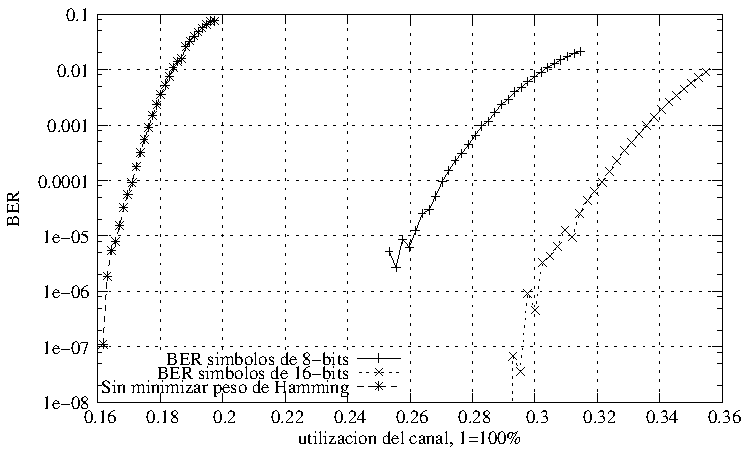
\includegraphics[width=6in]{graphs/BERvsChannelES2}
    \caption{Performance del sistema con respecto a la expansión de símbolo. Simulación numérica de un enlace de 10 Gbps con 128 clientes, M=4096 y K=9.}
    \label{BERvsExpansion}
\end{figure}

La Figura \ref{BERvsExpansion} muestra tres simulaciones: una sin expansión, otra con una expansión de 8 bits y otra de 16 bits. En dicha figura se muestra el BER en función de la utilización del canal (el porcentaje real de uso por la totalidad de los clientes cuando se elimina todos los bits extras de las codificaciones, es decir, la capacidad que la suma de usuarios vería sin este sistema). Como se puede apreciar, hay una mejora substancial en el aprovechamiento del canal: para un BER de $10^{-6}$ tenemos 0.16, 0.25 y 0.3 aproximadamente. Es decir que con 8 bit mejoramos un $50\%$ del original, y con 16 bis un $87\%$.


\section{Probabilidad de colisión de filtro de Bloom con expansión de símbolo}

%newJIS_140512
En esta sección, presentaremos una estimación analítica de la probabilidad de error de bit, tomando en cuenta sólo las interferencias de otros usuarios en la red.
No consideraremos ninguna corrección de etapas o algoritmos adicionales como Reed-Solomon, o interferencias producidas en el medio físico.
Como se explicó en la sección \ref{Bloomf}, cada usuario agrupa sus bits de información en paquetes o tramas de largo $n$. Cada paquete es codificado utilizando exactamente $m_{1}$ unos y $m_{0}$ ceros, siendo $m$ la cantidad de bits de la trama, donde $$m=m_{1}+m_{0}$$.

Debido a la utilización del filtro de Bloom, cada uno de los $m$ dígitos binarios resultantes es repetido $K$ veces en posiciones elegidas aleatoriamente en la trama de largo $M$. Las K repeticiones de un dígito binario pueden colisionar con otras repeticiones del mismo dígito, con repeticiones de otro dígito o bien con dígitos pertenecientes a otro cliente.
Llamaremos $N$ al número de usuarios activos. Para estimar la tasa de error o BER (Bit Error Rate) del sistema y simplificar los cálculos, asumiremos lo siguiente:

\begin{enumerate}
 \item Las tramas de diferentes usuarios están sincronizadas, es decir, cada usuario participante del canal de comunicaciones recibe la misma trama en el mismo orden, y cada trama contiene (incluyendo colisiones) $W_0 = N\cdot K\cdot m_0$ ceros y $W_1 = N\cdot K\cdot m_1$ unos.
 \item No incluiremos en el análisis la posibilidad de corrección de errores debido a que, en general, 
 \begin{equation}
\nchoosek{m}{m_1} > 2^n.
\end{equation}
Específicamente, cada vez que una secuencia errónea de $m$ dígitos binarios es recibida con más de $m_1$ unos, se decodifica como una cadena de bits aleatoria de largo $n$.
Por lo tanto, el número esperado de errores será $n/2$.
\end{enumerate}

Definiremos las siguientes probabilidades: 
$P_{s1}$ como la probabilidad de sobre-escribir con unos las $K$ repeticiones de por lo menos uno de los $m_0$ ceros.
$P_{st}$ como la probabilidad de sobrescribir con unos todas las $K$ repeticiones de uno de los $m_0$ ceros.

Entonces, el BER está dado por
\begin{equation}
%\text{BER} = \frac{n}{2}\prob{\text{sobre-escribir con unos las $K$ repeticiones de por lo menos uno de los $m_0$ ceros}}.
\text{BER} = \frac{n}{2}P_{s1}.
\label{eq:ber_01}
\end{equation}
Por la cota de la unión (union bound), 
%\begin{multline}
\begin{equation}
%\prob{\text{sobrescribir con unos las $K$ repeticiones de por lo menos uno de los $m_0$ ceros}}\leq \\
%\leq m_0\prob{\text{sobrescribir con unos las $K$ repeticiones de uno de los $m_0$ ceros}}.
P_{s1}\leq P_{st}.
\label{eq:union_bound}
\end{equation}
%\end{multline}
Por lo tanto, prestemos atención a uno de los $m_0$ ceros. Si los $W_{1}$ transmitidos (por todos los usuarios) ocupan $s$ casilleros y las $K$ repeticiones del cero dado usa $r ( \leq K)$ casilleros, entonces una condición necesaria para el error es que $s \geq r$. Entonces, asumimos que existan $s$ unos en una trama de $M$ bits. Dados $r$ lugares en la trama, la probabilidad de que los unos ocupen esas $r$ posiciones está dada por 
\begin{equation}
z_{r,s} = \frac{\nchoosek{M-r}{s-r}}{\nchoosek{M}{s}}= \frac{\frac{(M-r)!}{(M-s)! (s-r)!}}{\frac{M!}{(M-s)!s!}} = \frac{(M-r)!}{M!}\frac{s!}{(s-r)!}\approx (\frac{s}{M})^r,
\end{equation}

Suponiendo que $N,s\gg r$, si $M \gg K$, no es difícil ver que las $K$ repeticiones de un cero dado ocupan $\mu_{R} \approx K$ casilleros en promedio. También puede demostrarse que el número promedio de casilleros ocupados por los $W_{1}$ unos transmitidos por todos los usuarios es

\begin{equation}
\mu_{S} \approx M (1-e^{-W_1/M})
\end{equation}
 
De esas ecuaciones, una estimación de la cota superior del BER para un determinado usuario es
\begin{equation}
\text{BER} \approx \frac{n}{2} m_0 z_{\bar{R},\bar{S}} \approx \frac{n}{2} m_0 \left(1-e^{-W_1/M}\right)^K.
\end{equation}

La figura \ref{BERvsK} muestra la estimación en función de $K$ para $M=2014$, $m_{0} = 22$, $m_{1} = 2$, $n = 8$ y $N=38$. Es interesante notar que existe un valor óptimo de la tasa de repetición $K$ que minimiza la tasa de error. Este resultado es relevante en el diseño de un sistema de comunicaciones. Debido a los bajos valores de BER alcanzados, es posible utilizar en la siguiente etapa algoritmos eficientes que aceptan bajos límites de error, tal como Reed-Solomon, para reducir aún mas el BER total de sistema y asi llevarlo a tasas aceptables para aplicaciones prácticas.

\begin{figure}[!t]
  \centering
    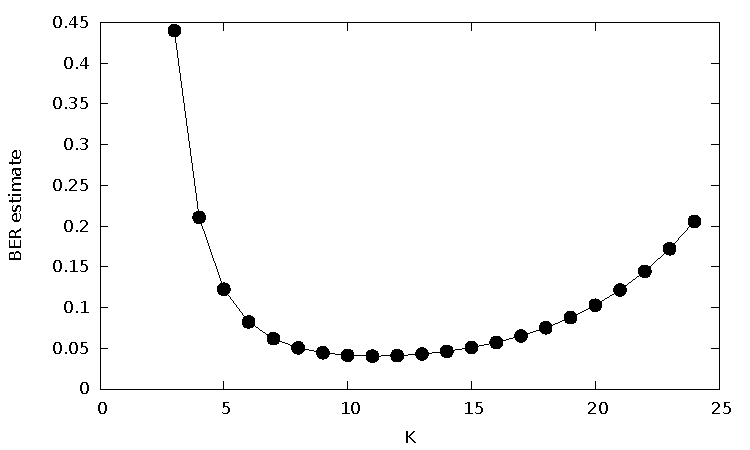
\includegraphics[width=5in]{graphs/Kcalc}
    \caption{Estimación de BER vs. tasa de repetición de filtro de Bloom K.}
    \label{BERvsK}
\end{figure}

\section{Códigos de pseudoruido}
Como se explica en la sección \ref{PRNGs} la seguridad del sistema depende de la correcta selección e implementación de un algoritmo de PRNG criptográficamente seguro \textit{(CS-PRNG)}.
El sistema impone una restricción adicional a esta etapa, ya que además de cumplir con todas las propiedades de un CS-PRNG, se debe seleccionar un algoritmo eficiente ya que se necesitará generar una posición aleatoria por cada bit que se desea transmitir. Por lo tanto, es deseable maximizar la cantidad de bits por ciclo de reloj que el CS-PRNG es capaz de generar.
En el caso de la implementación para el transceptor óptico sobre una FPGA, el algoritmo seleccionado para el prototipo inicial fue el denominado ARC4, debido a la simplicidad, bajo consumo de recursos de hardware y alta velocidad del mismo  \cite{Menezes:1996:HAC:548089}. Si bien existen implementaciones de alta performance \cite{10.1109/TC.2012.19}, estas no son fácilmente accesibles ni disponibles, por lo que se reimplementó este algoritmo íntegramente, utilizando el lenguaje de descripción de hardware Verilog \cite{thomas2002verilog}, utilizando optimizaciones para lograr la performance deseada de 1 byte pseudoaleatorio generado por cada ciclo de reloj. Es necesario tener en cuenta es que ARC4 es un algoritmo relativamente anticuado y recientemente varios ataques estadísticos han puesto en duda su utilización como generador criptográficamente seguro \cite{Sepehrdad:2011:SAR:2008684.2008712}, por lo que en implementaciones futuras es recomendable que sea reemplazado por un algoritmo criptográfico moderno.

En las implementaciones de software o acústicas, el poder de procesamiento necesario para esta etapa se reduce, ya que la velocidad de reloj de un CPU suele ser elevada con respecto a la velocidad posible en este medio de trasmisión, por lo que no es necesario que el algoritmo PRNG tenga un rendimiento elevado.


\subsection{Aplicación al algoritmo de filtro de Bloom encriptado}

Este algoritmo asigna los tiempos de transmisión de $r$ clientes, seleccionándolos entre $M$ posiciones, correspondientes a los $M$ casilleros dentro de la trama de transmisión.
La cantidad posible de combinaciones de $M$ posiciones entre todos los clientes es de $ _{M}P_{r} = \frac{M!}{(n-r)!} $.
Consideraremos que un ataque a este algoritmo fue exitoso cuando un atacante puede inferir la serie de posiciones $M$ para un cliente, obteniendo así todos sus datos.

Existe un algoritmo de selección de $M$ que suponemos no posee ninguna debilidad, es decir, selecciona $r$ conjuntos de $M$ posiciones tal que, aún si el atacante pudo adquirir un número arbitrario de las posiciónes de transmisión pasadas, no puede predecir ninguna de las posiciones futuras.

Esto puede cumplirse simplemente asignando a cada canal de transmisión seguro su propio algoritmo generador pseudoaleatorio criptográficamente seguro, o bien el mismo algoritmo utilizando claves diferentes. Esto provocará colisiones entre los clientes, es decir, al asignarse posiciones de transmisión de manera aleatoria, existirán coincidencias donde a dos o más clientes se les asignará el mismo casillero dentro de la trama. Esto es resuelto mediante corrección de errores en capas superiores y para el cálculo del parámetro de seguridad se despreciará este efecto.

Dadas las siguientes suposiciones:
\begin{itemize}
 \item El algoritmo de selección pseudoaleatorio no tiene debilidades.
 \item El atacante no posee control de los datos a transmitir, y estos son totalmente aleatorios.
\end{itemize}

Un atacante podria tratar de predecir el conjunto de posiciones $n$ de un cliente, para obtener sus datos. Para ello, deberá probar exhaustivamente todo el conjunto de $ _{M}P_{r}$ sobre una trama capturada, o bien probar todas las combinaciones posibles de la clave del generador pseudoaleatorio. De esto se desprende que si $largo(clave)>128\ bits$ y $M>128$ se considera que el algoritmo cuenta con un nivel de seguridad denominada ``fuerte'', ya que una complejidad temporal de $2^{128}$ es considerada segura al momento de la escritura de esta Tesis \cite{eastlake2005s}.

\subsection{Problemas de símbolos con peso de Hamming variable}
En la sección anterior se nombraron dos condiciones necesarias. La primera condición, la carencia de vulnerabilidades en el algoritmo CS-PRNG, es necesaria e inevitable por motivos obvios. Sin embargo, es posible eliminar la segunda condición, de precisar datos totalmente aleatorios, realizando una modificación a la tabla de expansión. Esto es posible ya que la segunda condición es sólo necesaria para prevenir el siguiente escenario donde la seguridad falla:

Supongamos que se desea transmitir dos bytes:
\begin{itemize}
 \item El byte 0 ($00000000$ en representación binaria) 
 \item Y el byte 255 ($11111111$ en representación binaria)
 \end{itemize}

La tabla de expansión convierte los símbolos de 8 bits en símbolos de 16 bits, con peso de Hamming $HW<=2$.
Supongamos que la tabla asignó al valor 0, el símbolo $0000000000000000$ y al valor 255 el símbolo $0000100010000000$. Ambos símbolos de salida cumplen con la condición de $HW<=2$. Al transmitirse estos bytes, las posiciones son aleatorizadas y transmitidas.

Ignorando momentáneamente las colisiones, un atacante que observa el tráfico puede reconocer qué byte esta siendo transmitido, aún cuando la posición de cada bit este aleatorizada, simplemente contando la cantidad de unos, es decir, el peso de Hamming variable está revelando al atacante información acerca de los datos transmitidos, aún cuando los símbolos fueron permutados.

Éste ataque puede eliminarse generando una tabla de expansión cuyo peso de Hamming de símbolos de salida sea estrictamente un valor fijo. Es decir, para evitar el ataque en el ejemplo anterior, los símbolos de salida en lugar de tener $HW<=2$ deben cumplir con la condición de $HW=2$. 

De esta manera, al convertir los datos de entrada en símbolos uniformes con el mismo largo y el mismo peso de Hamming \footnote{Si el peso de Hamming es $P$, el atacante podrá observar un peso de Hamming de $1$ hasta $P$, y no siempre $P$, esto es debido a las colisiones de bit que un símbolo transmitido por un cliente tendrá con sí mismo.}, los bits de salida del algoritmo serán completamente aleatorios sin importar los datos de entrada y el atacante no podrá inferir ninguna información acerca de la comunicación.

\section{Resumen del sistema completo}
%% De orte.tex
El sistema propuesto, cuyo diagrama de alto nivel se muestra en la figura \ref{fig_comstack}, está compuesto primeramente de una capa de acceso, donde se encuentra la implementación de la codificación CDMA y la corrección de errores, y una capa física basada, o bien en una red óptica con similitudes a redes PON \ref{defPON} , o una red acústica de tipo difusión (\textit{broadcast}).
La capa de acceso está implementada utilizando técnicas CDMA del tipo time-hopping, donde cada uno de los clientes posibles codifica su información en bits y los transmite en un casillero seleccionado de manera aleatoria dentro de una trama de $M$ casilleros\footnote{ El parámetro $M$ debe optimizarse en función del nivel de error aceptable y la máxima cantidad de clientes soportados.}. De esta manera, ocurrirán múltiples colisiones entre diferentes ONUs \textit{(optical network unit)}, pero los errores causados por estas colisiones serán corregidos por la capa de corrección que garantiza una transmisión de datos confiable. Aunque es imposible eliminar totalmente los errores, consideramos una transmisión con un BER de 10e-12 como libre de errores.

Si bien existe el requerimiento de que todos los clientes comunicantes deben estar sincronizados a nivel de trama para regenerar correctamente las posiciones de transmisión, esta sincronización no es necesaria para clientes que no participen del canal encriptado.
Un cliente $X$ puede recibir mensajes de otro cliente $Y$ si y sólo si $X$ posee la {\em clave} de $Y$, y viceversa. De esta manera, si un cierto grupo de clientes desea comunicarse sobre un canal encriptado, es necesario cada cliente en el grupo conozca la {\em clave}. El canal encriptado que se forma entre los clientes forma un ``dominio de difusión'' ya que todos los datos que transmita un cliente serán recibidos sólo por los otros clientes participantes del dominio. Este dominio es análogo al sistema VLAN \textit{(Virtual Local Area Network)} de particiones lógicas de red.

Los datos de los clientes se codifican con las siguientes técnicas de corrección de errores: Reed-Solomon ($223/255$) (ver \cite{Moon:05} y sus referencias), y un filtro de Bloom\cite{Bloom70space/timetrade-offs}. 

En principio, se utilizó un algoritmo LDPC \ref{defLDPC} (Con matriz de $1024\times512$) pero fue descartado en posteriores iteraciones del diseño, ya que al agregar la optimización de la expansión de símbolo al filtro de Bloom, se incrementó la capacidad de corrección del mismo y pudo eliminarse la etapa de corrección de errores de tipo LDPC, con el consiguiente aumento de la capacidad total del sistema.

En la selección de los algoritmos de corrección de errores siempre se utilizó el canal Z como modelo del canal de comunicaciones. %que posee un limite de Shannon de $ C_{Z} = \log_2\left(1+(1-p) p^{p/(1-p)}\right),$ donde $p$ es la posibilidad de recibir un error al transmitir un bit. Este limite de capacidad es menor que el límite en una canal simétrico sin memoria \cite{Tallini:02}.

\section{Aplicación en distintos medios físicos}
Al poseer una fuerte capacidad de corrección de errores, la arquitectura del sistema lo hace confiable frente a todo tipo de interferencias de la capa física, por lo que modificando la etapa de modulación pueden utilizarse diferentes medios físicos, siempre que los mismos puedan modelarse como un canal Z.
\begin{figure}[t]
  \centering
      \subfloat[Distribución via acoplador tipo estrella 1]{{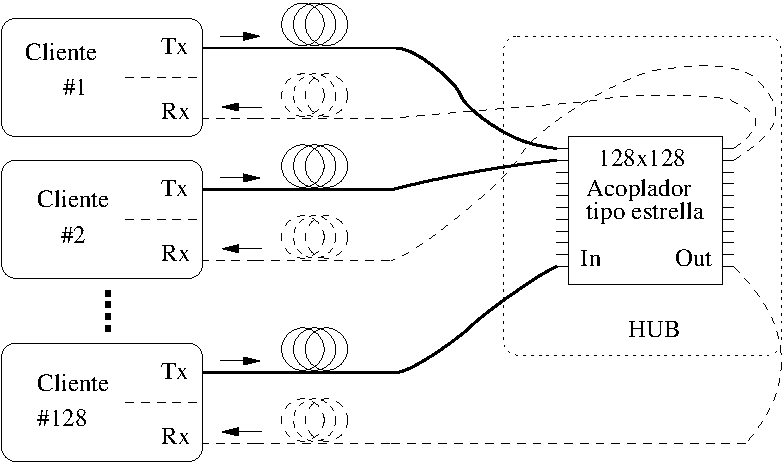
\includegraphics[width=0.62 \textwidth]{graphs/StarCoupler} }}%
    \qquad
    \subfloat[Distribución via EDFA]{{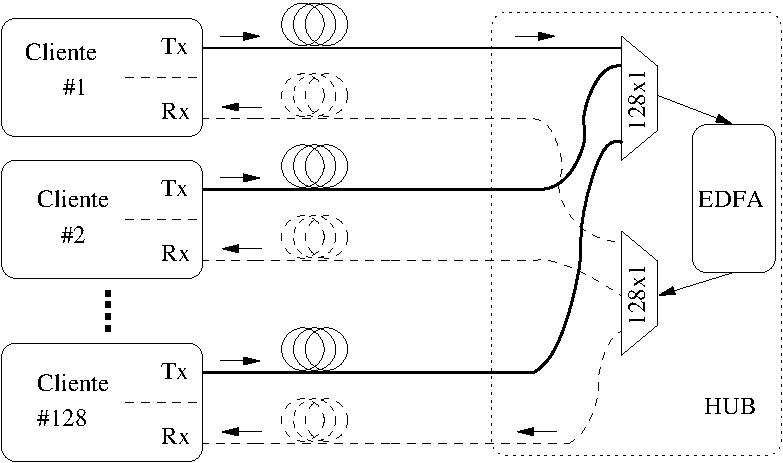
\includegraphics[width=0.62 \textwidth]{graphs/EDFA} }}%
    \caption{Diseño de red propuesto para la capa óptica: un acoplador de tipo estrella es la base para la arquitectura de red en distancias inferiores a $10~\mathrm{km}$. Para extender el alcance de la red, un amplificador óptico del tipo EDFA \textit{(Erbium-Doped Fiber Amplifier)} puede ser utilizado en el concentrador central.}
    \label{arch:fig1}
\end{figure}

\subsection{Redes ópticas}
% de orte.text



%\begin{figure}[t]
%  \centering
%  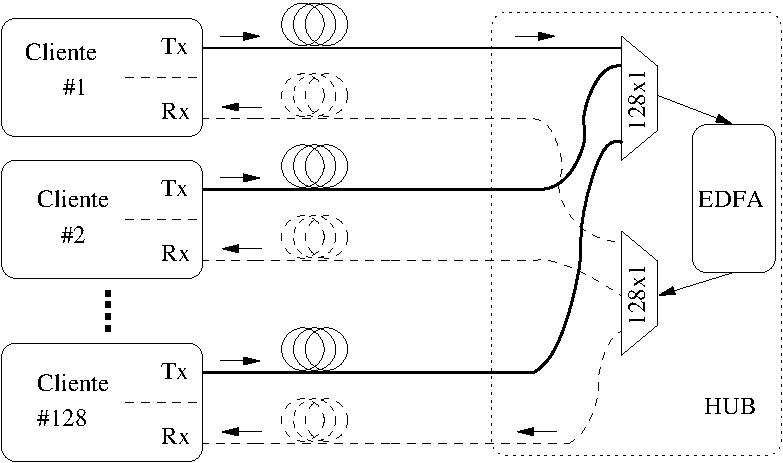
\includegraphics[width=0.48 \textwidth]{graphs/EDFA}
%  \caption{Para distancias superiores a $10~\mathrm{km}$ la red requiere amplificación provista por un EDFA.}
%  \label{arch:hub_edfa}
%\end{figure}


%\begin{figure}[!t]
%  \centering
%    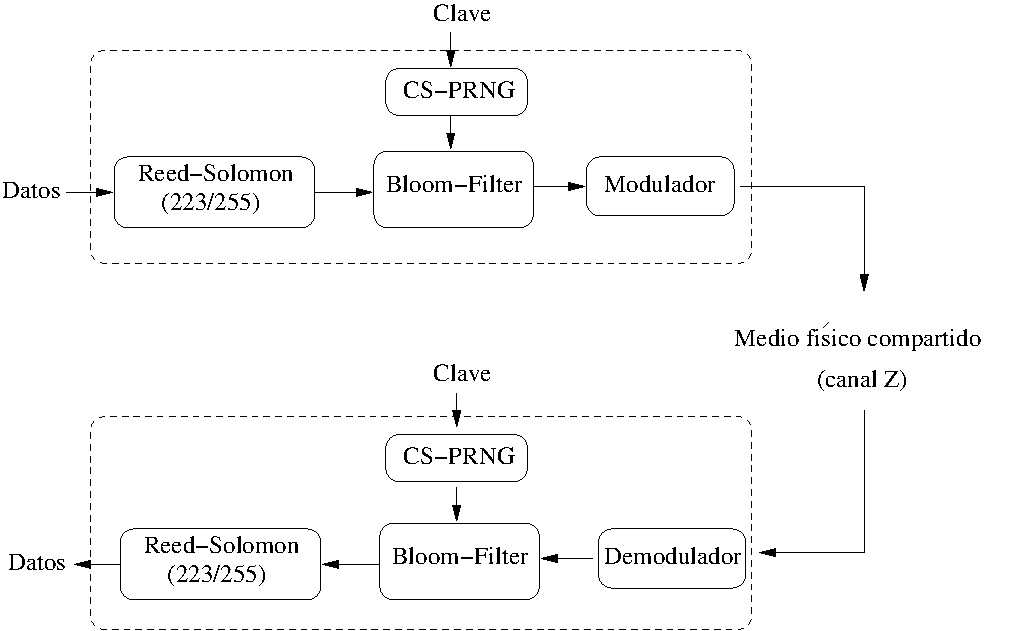
\includegraphics[width=5in]{graphs/Soft-stack3}
%    \caption{Diseño de red propuesto: Pila de comunicaciones}
%    \label{arch:chain}
%\end{figure}
% Fiber		Es grave el efecto de la dispersion?  Sugerimos dispersion shifted G.653? O son muy caras?
% splitter	No 1x128 commercially available (attenuation $\leq 27\,dB$)
% DFB		http://cess-dk.com/gfx/upload/PX2-1541SF.pdf ( min $\simeq-1\,dB$)
% APD		http://pdf.dzsc.net.cn/200810212/286762.pdf ( max $\simeq-27\,dB$)
% EDFA		http://www.lambdaphoto.co.uk/pdfs/EDFADatasheet.pdf

Al adaptar el sistema propuesto a una red óptica, la topología física debe ser de tipo estrella (ver Fig.\ref{arch:fig1}) donde splitters ópticos redistribuyen el tráfico proveniente de cada ONU a todo el resto de los terminales, permitiendo comunicaciones punto a punto así como punto a multipunto, con una cantidad máxima de hasta $128$ ONUs simultáneas. Este límite esta dado por las atenuaciones causadas por la fibra óptica y por el concentrador que el sistema debe ser capaz de compensar mediante amplificación.

%Traffic redistribution is made by optical splitters at the redistribution hub that introduces high attenuation to optical streams.
Un amplificador óptico de tipo EDFA \textit{(Erbium-Doped Fiber Amplifier)} localizado entre los splitters incrementa la potencia óptica para compensar las perdidas en la red, aunque esto es solamente necesario en distancias entre clientes superiores a 10 km.

La modulación utilizada para las señales ópticas es RZ o \textit{Return to Zero}, con velocidades previstas de hasta $10$~Gbps, utilizando un Láser DBF \textit{(Distributed Feedback)} de $2$~dBm de potencia y $1550$~nm de color/frecuencia. Estos parámetros permiten una transmisión de hasta $10$~km entre los nodos si se utiliza fibra óptica mono modo estándar (ITU-T G.652).

En el concentrador, un splitter de $128\times 1$ concentra el tráfico de todos los ONUs y es luego redistribuido por el correspondiente splitter de $1\times 128$, canalizando el tráfico combinado de cada ONU a través de las fibras ópticas. Este splitter permite tener hasta 128 ONUs en el sistema.

La atenuación de los splitters centrales ($\simeq25$~dB cada uno) sumada a la atenuación propia de la fibra óptica ($\simeq2$~dB por tramo) y pérdidas por inserción (aproximadamente $\simeq1$~dB) contribuyen a la elevada atenuación que el amplificador debe compensar ($\simeq28$~dB).

De utilizarse sin ningún tipo de amplificación, la atenuación que una señal sufriría entre dos ONUs es la suma de la atenuación de ambos tramos, es decir $\simeq56$~dB, que es un valor que supera el límite de la tecnología de detección comercial disponible al momento de la escritura de esta Tesis, teniendo en cuenta potencias de transmisión máximas de 2 dBm.

Sin embargo, es posible utilizar etapas de amplificación intermedias para obtener niveles de señal adecuados. Para proveer la amplificación requerida, un EDFA con $\geq27$~dB de ganancia es colocado entre ambos splitters. Este EDFA incrementa la potencia del tráfico a la salida del primer splitter, elevando la potencia de cada '1' de $\simeq-26$~dBm a $1$~dBm a la entrada del segundo splitter, que será atenuada nuevamente a un nivel de potencia de $-27$~dBm, valor dentro de los parámetros aceptables de un fotodetector de alta sensibilidad (aproximadamente $-28$~dBm~\cite{comapd}).

%La potencia máxima de salida del PD no es un parámetro crítico ya que simulaciones [CUALES?] muestran que solamente se producirán colisiones de hasta diez `1' en un casillero, y esto con una posibilidad extremadamente baja. -- eliminado por carencia de simulaciones

Aún considerando una ganancia de EDFA constante, la potencia óptica a la entrada del detector PD sería menor ($-17$~dBm) que la requerida por dispositivos comerciales ($\sim -5$~dBm).
El nivel de bit `0' es dado por la adición de todos los bits `0' transmitidos por las $128$~ONUs. Por lo tanto, el nivel de decisión del receptor debería ser capaz de separar entre este estado (la suma de los bits `0') y aquel de un simple ONU transmitiendo un solo bit en `1'.
De esto se desprende que la potencia de transmisión del bit `0' debe ser la menor posible, o lo que es lo mismo, la \textit{relación de extinción} del láser DBF debe ser alta.
%El radio de extinción (`1'$/$`0' radio de potencia pico) mínimo requerido por el sistema se discute en las simulaciones numéricas a continuación:

% As collisions occur in this scheme minimal powers are such for the case of a single active Tx in a bit casillero. In a bit casillero with collisions (two or more `1' bits) power increase could be a concern to APD operation
% Optical transmission is performed by a $2$~dBm $1550$ nm DFB-laser generating a
% $10$ Gb/s RZ modulated optical signal, that is transported by up to $10$
% km upstream fiber (ITU-T G.652) to a redistribution hub (see
% Fig.~\ref{arch:fig1}).
% Upstream traffic from all ONUs are merged by a $128\times 1$ splitter and then again redistributed by another splitter $1\times 128$ that channels back merged traffic to each ONU through a downstream fiber identical and parallel to the upstream one.
% Splitters' attenuation ($\simeq25$~dB, estimated) contribute, as well as fiber attenuation and insertion losses ($\simeq2$~dB and $\simeq1$~dB per stretch), amount to high total attenuation ($\simeq28$~dB at each upstream and downstream paths).
% In order to make the system workable it is proposed to place a single EDFA optical amplifier ($\geq27$~dB gain) between both splitters.
% This EDFA rises merged traffic power at first splitter output ($\simeq-26$~dBm `1' active Tx) delivering enough power ($1$~dBm, `1' active Tx) at second splitter input to assure power reaching each ONU ($-27$~dBm, `1' active Tx) allows proper reception by a high sensitivity APD ($-28$~dBm).

\subsection{Redes acústicas}
% de newJIS_140512-1.pdf (paper JIS)
\begin{figure}[!t]
  \centering
    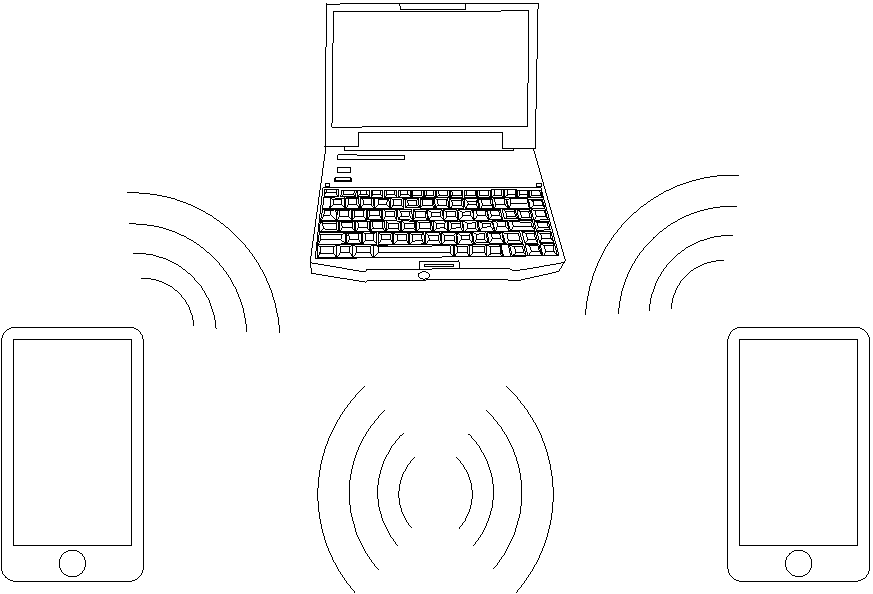
\includegraphics[width=4.5in]{graphs/compucelus.pdf}
    \caption{El diseño de red acústica propuesta puede contener nodos heterogéneos, tales como teléfonos del tipo smartphone o computadoras personales.}
    \label{arch:chain}
\end{figure}

Un canal óptico es un claro ejemplo de canal Z, pero también es posible realizar un canal Z con redes acústicas si se utilizan ciertas modulaciones.

Los enlaces ópticos presentan como mayor desventaja la necesidad de, o bien transmitir los pulsos de luz mediante una fibra óptica entre los nodos comunicantes, o que exista visibilidad directa entre ambos nodos, una condición que no puede ser garantizada en todos los ambientes de trabajo. Además, los sensores ópticos requeridos generalmente no están presentes en los clientes y deben ser instalados separadamente.

Sin embargo, la transmisión sobre un canal acústico tiene como ventaja el poder utilizar hardware instalado en la mayoría de los potenciales clientes, tales como parlantes o micrófonos estándar, elementos comunes en dispositivos electrónicos masivos \cite{citeulike:12800468}. Además, no es necesaria la visibilidad directa mientras ambos nodos estén localizados a pocos metros de distancia.

En contraste con otras tecnologías como RF o enlaces ópticos, la naturaleza del canal acústico y la facilidad para interceptar o registrar comunicaciones utilizando este medio hace de la privacidad un requerimiento esencial. Algunos sistemas de comunicación de audio han sido propuestos \cite{august2002apparatus}, pero el problema de la privacidad en este tipo de comunicaciones se soluciona generalmente en la capa de aplicación, es decir, en alto nivel. Esta Tesis presenta una aproximación a la seguridad y privacidad desde la capa física, basada también en time-hopping CDMA, similar a aquella presentada en \cite{6476559}. Presentaremos una red segura acústica punto a punto y punto a multipunto de corto alcance y bajo consumo, que no requiere de ningún hardware adicional en clientes móviles.

Un escenario válido para la aplicación de esta tecnología podría ser validación de transacciones financieras pequeñas tales como terminales PoS \textit{(Point of Sale)} o cajeros automáticos (ATM) utilizando un dispositivo móvil (por ejemplo, un celular del tipo \textit{smartphone}) sin modificaciones de hardware. Una tecnología similar que se utiliza en estos casos es la denominada NFC \textit{(Near Field Communications)} \cite{nikitin2007overview}, un protocolo inalámbrico que requiere hardware especializado que, al momento presente, no se encuentra disponible en la mayoría de los dispositivos móviles.
Con respecto a la implementación sobre el medio óptico, es necesario ajustar algunos parámetros, como por ejemplo el tamaño de trama, que se reduce de $M=4096$ a $M=256$ para la implementación acústica, y el parámetro $K=9$ que es el óptimo para el $M$ seleccionado. El número de clientes también se ve reducido de $N=128$ a $N=12$ ya que al ser la red acústica de corto alcance, no se prevé una elevada cantidad de clientes simultáneos. En la figura \ref{arch:AudioSimul} se muestra una simulación del sistema con estos parámetros contrastada con una medición realizada entre una Notebook (T420) y un celular (Lenovo A789).  En dicha figura se puede apreciar que las simulaciones y las mediciones son similares, mostrando estas últimas desde 14 clientes en adelante. La razón por la cual sólo se muestra a partir de 14 clientes reside en que la tasa efectiva de transmisión es muy baja y para medir un BER más grande, se necesitaban tiempos del orden de un día. Teniendo en cuenta que este tipo de sistemas se utilizarían para transacciones de pocos bytes, y la coincidencia entre la curva simulada y la real, consideramos que el desempeño es adecuado.

\begin{figure}[t]
  \centering
    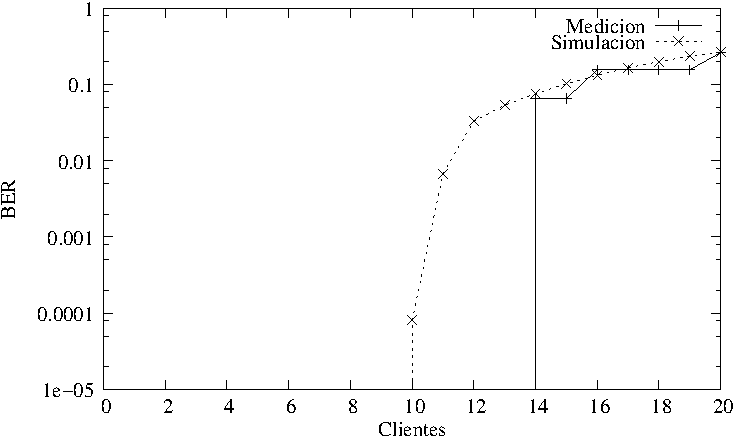
\includegraphics[width=5in]{graphs/audio-fig6}
    \caption{Simulación y medición del BER para una red acústica en función del número de clientes con M=256 y K=9.}
    \label{arch:AudioSimul}
\end{figure}



\subsection{Redes acústicas: arquitectura}

Una ventaja importante del sistema acústico propuesto es su simplicidad, requiriendo solamente un emisor de sonido (parlante), un receptor (micrófono) y un canal de transmisión de sonido que puede ser aire (y, en casos más especializados, agua). Ambos requerimientos están generalmente disponibles en computadoras, notebooks, tablets y teléfonos celulares. 
El esquema lógico es el mismo que el descrito anteriormente: time-hopping CDMA seguro, códigos correctores de errores y un método de sincronización a nivel de bit.
Como resultado, el sistema soporta canales unidireccionales a los clientes que sirven tanto para comunicaciones punto a punto como punto a multipunto. 
Para la implementación de canales bidireccionales, pueden utilizarse dos canales separados (ej. utilizando dos códigos CDMA diferentes), o empleando el mismo canal de manera \textit{half duplex}, aunque este último modo de funcionamiento necesita de desarrollo adicional y no es el objetivo de esta Tesis.
En las próximas secciones se describe el sistema en mayor detalle.

\subsection{Redes acústicas: modulación y sincronización}
\begin{figure}[t]
  \centering
    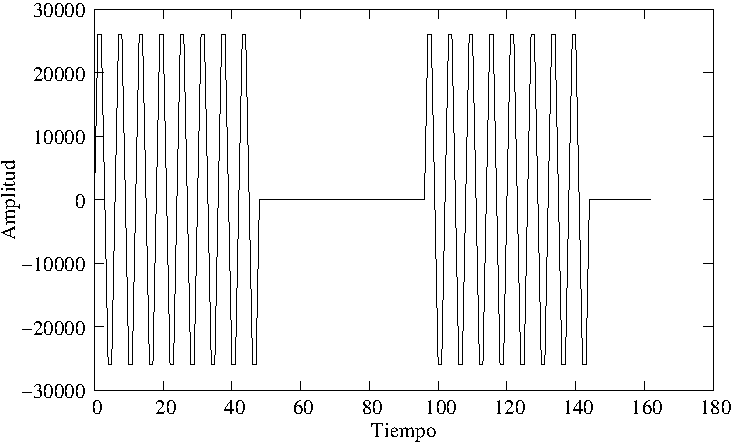
\includegraphics[width=5in]{graphs/modulated.pdf}
    \caption{Modulación OOK.}
    \label{arch:ook}
\end{figure}


A diferencia de la implementación óptica donde se utilizaron algunas funciones provistas por el hardware de FPGA, tales como el mecanismo de sincronización de bit, para la transmisión acústica se implementaron tanto el algoritmo de modulación como el de sincronización totalmente en software.
Para la modulación, fue utilizado el algoritmo de OOK (ver Fig. \ref{arch:ook}), que codifica los bits a transmitir como pulsos. La frecuencia de portadora puede variar de 10 kHz a 16 kHz, y la tasa de transmisión se fijo a 1000 bps. Debido a la baja velocidad de este canal se introduce un problema inexistente en la implementación óptica: el retraso de la red (el tiempo que tarda un bit en atravesar toda la red) es alto, debido principalmente a la etapa de Reed-Solomon que necesita recibir 256 bytes para comenzar el proceso de decodificación del bloque. Debido a que el canal soporta una velocidad máxima de 1000 bps, el retraso puede alcanzar niveles inaceptables, del orden de los 30 segundos.
Una selección mas apropiada del algoritmo de FEC (tal como BCH) podría reducir reducir el retraso total del sistema.
Adicionalmente, una etapa de \textit{pulse shaping} o formación de pulso fue implementada, utilizando un filtro pasa-banda a la salida de la modulación y también en la entrada del demodulador. Este filtro ayuda a rechazar interferencia acústica o ruido ambiente.

\begin{figure}[t]
  \centering
    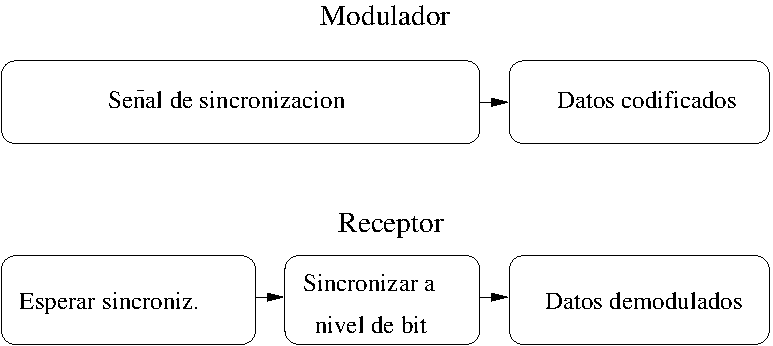
\includegraphics[width=4.5in]{graphs/Audio-Sync2.pdf}
    \caption{Sincronización.}
    \label{arch:sync}
\end{figure}


La sincronización entre un transmisor y un receptor es esencial para la decodificación correcta de la información. Por esta razón, un patrón de sincronización inicial es enviado, para que el receptor pueda ajustar parámetros tales como la fase y nivel de decisión de la señal (ver Fig. \ref{arch:sync}). La deriva \textit{(drift)} del reloj y variabilidad \textit{(jitter)} no son significativas a esta baja velocidad de transmisión y ninguna corrección en tiempo real es requerida, por lo que la implementación del módem por software es simple.
El nivel de decisión del demodulador es dinámico, es decir que es constantemente recalculado utilizando los niveles de entrada promediados.
La fase del símbolo recibido también es corregida utilizando los mismos datos de entrada como referencia.


\chapter{Resultados experimentales: medios de transmisión óptica y acústica}
\label{simulations}
En este capítulo se muestran resultados numéricos y experimentales de la implementación del esquema de seguridad propuesto, para los diferentes módulos y el sistema completo, en medios de transmisión ópticos y acústicos. 
\section{Implementación en software}
Como paso previo a realizar las implementaciones sobre FPGA en el caso óptico, y sobre software en el caso acústico, se implementaron simuladores numéricos de todas las etapas, y se combinaron para comparar los resultados con los teóricos. El simulador fue programado utilizando el lenguaje de C/C++. Fue necesario utilizar este tipo de lenguaje de alto rendimiento debido a que se necesitan simular grandes cantidades de datos para realizar mediciones de tasas de error del orden de 10e-8. Específicamente, en cada paso de simulación se transmite más de 1 Gb de datos por cliente, con hasta 128 clientes, por lo que se requiere del mayor rendimiento posible para obtener tiempos de ejecución aceptables.

\subsection{Estructura general}

La estructura general del simulador es modular, con una separación de alto nivel que obedece al diagrama lógico que puede verse en la figura \ref{fig_comstack}.
Cada módulo representa una etapa en el sistema de comunicaciones que realiza una transformación específica sobre los datos, que puede ser modulación, demodulación, corrección de errores, etc. Los diferentes módulos actúan como filtros, recibiendo y enviando los datos transformados utilizando la entrada y salida estándar del sistema operativo (STDIN/STDOUT). La simulación comienza con un bloque generador de datos binarios aleatorios.

Estos datos son alimentados a la segunda etapa, que es el módulo de corrección de errores. La salida codificada de este módulo es posteriormente alimentada a la siguiente etapa, y de esta manera, los datos originales son sucesivamente transformados en cada módulo.


El medio de transmisión físico es también simulado mediante un modulo que simula las características físicas del canal seleccionado; por ejemplo, en el modulo de simulación óptica, se tienen en cuenta la dispersión y la atención de la señal introducidas por la fibra óptica.

Al llegar a la simulación de la última etapa de la recepción, donde deberían obtenerse los datos originales, el resultado es comparado bit a bit con los datos introducidos originalmente y, en base a las diferencias detectadas, se calcula y reporta el BER. Esta estructura modular brinda flexibilidad al simulador, permitiendo introducir y remover etapas fácilmente.

Sigue a continuación una lista de los módulos y sus características relevantes:

\begin{description} 
 \item[rsenc/rsdec] Codificador/Decodificador de la etapa de corrección de errores. Específicamente, se implementa el algoritmo Reed-Solomon. Es posible generar un código ``recortado'' especificando la cantidad de bytes por bloque en el primer argumento.
 \item[scrambler/descrambler] Implementación del scrambler de datos. El tamaño de bloque puede ser especificado en el primer argumento. Es recomendable que el tamaño de bloque sea un múltiplo del tamaño de bloque del corrector de errores (en nuestro caso, 255 bytes).
 \item[bfenc/bfdec] Etapa codificadora/decodificadora que utiliza el filtro de Bloom. Para simular la interferencia en el medio compartido, en esta etapa se genera un flujo de datos aleatorio por cada cliente a simular y se lo agrega a la trama, lo que provocará colisiones. El único argumento es la cantidad de clientes presentes en el canal.
 \item[noisesim] Simulador de ruido óptico y de distorsión de la señal en la fibra óptica. La tasa de transmisión esta fija a 10 Gb/s. El único parámetro especifica la cantidad de clientes interfiriendo la señal.
 \item[bin2wav/wav2bin] Modulador/Demodulador acústico. Transforma la señal de entrada en ondas acústicas con codificación PCM (\textit{Pulse Coded Modulation}). El módulo de sincronización de audio se encuentra dentro de la utilidad wav2bin.
\end{description}

En general, el simulador puede ejecutar cada etapa consecutivamente, donde cada módulo completará el procesamiento de datos antes de comenzar con la próxima etapa:

\small
\begin{verbatim}
 ./rsenc <${FILE} | ./scrambler ${SCRAMBLEBLOCK} >rs.out
 ./bfenc ${CLIENTES} < rs.out | ./noisesim -c ${CLIENTES} -r 16.6 >bfenc.out
 ./bfdec ${CLIENTES} <bfenc.out >bf.out
 ./descramble ${SCRAMBLEBLOCK} <bf.out | ./rsdec >rsdec.out
\end{verbatim}
\normalsize

En el ejemplo anterior, los módulos utilizan archivos temporales como forma de comunicación. Esto causa que cada módulo deba finalizar el completo procesamiento de los datos de entrada antes de que sean procesados por el módulo siguiente.

Una simple modificación al ejemplo anterior permite prescindir del uso de archivos temporales, mediante la ejecución paralela:
\small
\begin{verbatim}
./rsenc <${FILE} | ./scrambler ${SCRAMBLEBLOCK} | ./bfenc ${CLIENTES} | \
                 ./noisesim -c ${CLIENTES} -r 16.6 | ./bfdec ${CLIENTES} | \ 
                 ./descramble ${SCRAMBLEBLOCK} | ./rsdec > file.out
\end{verbatim}
\normalsize

En la primera configuración del simulador se puede acceder a los archivos temporales intermedios, útiles para depuración y mediciones por etapa, mientras que la segunda configuración tiene la ventaja de aprovechar la totalidad de los procesadores disponibles en el sistema, ya que en un sistema multiprocesador, el sistema operativo usualmente asigna un CPU a cada etapa y estas se ejecutan en paralelo.

La implementación sobre un medio acústico no presenta mayores inconvenientes con respectos a la velocidad de procesamiento, ya que las tasas de transmisión son bajas, acotadas naturalmente por el medio de transmisión y ancho de banda disponible, por lo que los recursos computacionales necesarios para la simulación son limitados. 
Utilizando el medio óptico, normalmente se necesita simular la transmisión de un gigabit o más para obtener una medición confiable del BER del sistema, ya que este medio tiene naturalmente una tasa de transmisión elevada y un BER pequeño, del orden de 10e-12. Adicionalmente, sobre este último medio el sistema soporta un máximo de 128 clientes que son simulados simultáneamente, por lo que los recursos computacionales requeridos son considerables. A raíz de este problema, y aprovechando que la simulación es altamente paralelizable, se implementó un sistema de estilo cliente-servidor donde los cálculos son distribuidos en un grupo de nodos.

\subsection{Etapa de corrección de errores/scrambler}

Los módulos de corrección de errores (rsdec/rsenc) fueron implementados utilizando bibliotecas de código abierto. Se utilizó la popular biblioteca libFEC del autor Phil Karn \cite{libfec}. En cuanto al los módulos de scrambler/descrambler, se implementó un algoritmo de scrambling que utiliza una matriz de permutación aleatoria generada mediante una semilla en cada ejecución, garantizando que las permutaciones sean reversibles.

\subsection{Implementación de filtro de Bloom}
El módulo bfenc/bfdec realiza la codificación/decodificación por software del algoritmo de filtro de Bloom. Los parámetros del algoritmo, tales como el tamaño del filtro $M$ y la cantidad de clientes a simular, son configurables. Una característica que merece mencionarse es la del sistema de minimización de peso de Hamming que es realizado en esta etapa. Tal como se explico en \ref{miniham}, la  implementación se implementó mediante una tabla de lookup (ver tabla \ref{hwtable}), lo que permite consultas muy eficientes con una complejidad temporal de $O(1)$, aunque el tamaño de la tabla (también llamado complejidad espacial del algoritmo) se aproxima a $O(2^{N})$, donde $N$ es la cantidad de bits por símbolo, por lo que para tamaños razonables de $N<24$, la tabla es autogenerada en cada ejecución en función de los parámetros necesarios.

\subsection{Simulador de medio acústico}

El medio de transmisión acústico fue simulado adoptando un modelo físico relativamente sencillo, que sólo toma en cuenta ciertas limitaciones en la respuesta en frecuencia. Para esto, se crearon módulos independientes que realizan la modulación, sincronización, demodulación y filtrado de la señal resultante.
Los módulos transforman los bits de entrada en una señal de audio digital con codificación PCM, a la cual se aplica un filtro pasa banda para simular las limitaciones en frecuencia de los transductores, que comúnmente son son los parlantes y micrófonos de un dispositivo móvil. Este módulo respeta el diseño de los anteriores, emitiendo la señal analógica como un flujo de bytes con codificación PCM vía la salida estándar del sistema. El filtro pasa banda fue implementado como un filtro digital de respuesta finita o FIR \textit{(Finite Impulse Response)}.
Este simulador utiliza algoritmos de modulación, filtros y sincronización reales, por lo que muchos módulos pudieron ser reutilizados sin modificaciones en un medio real. Para más detalles, ver sección \ref{redacus}.

\subsection{Simulador de ruido óptico} 
%% de orte.text

El modelo de simulación del canal óptico toma en cuenta tanto efectos lineales como no lineales en la fibra óptica. 

Se asume que el tráfico proveniente de todas las ONUs alcanza al divisor de $128\times1$ con perfecta sincronización de bit y sin fluctuaciones o \textit{jitter}.
Los casilleros correspondientes al bit `0' contienen una pequeña intensidad óptica de CW (\textit{Continous Wave}, potencia siempre presente en el láser) dada por el razón de extinción de Tx.
Debido a esta potencia óptica siempre presente, cada ONU agregado al sistema agrega una pequeña intensidad de bit `0', incrementando la potencia base total (ver figura \ref{sim:extinction}).
Para la simulación se asume que cada bit `1' agrega un pulso super-Gaussiano ($m=4$) al nivel de potencia base, con un ciclo de trabajo (\textit{duty cycle}) de $1/3$, una aproximación razonable a los parámetros utilizados por el transceptor multigigabit utilizado.

\begin{figure}[!t]
    \centering
      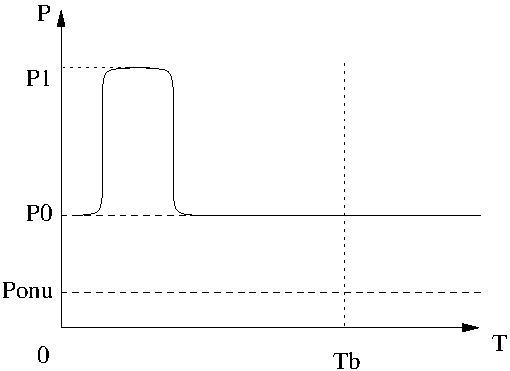
\includegraphics[width=3.5 in]{graphs/extinction.pdf}
      \caption{Diagrama de un bit supergaussiano (m=4) con ciclo útil de 1/4. La potencia del nivel del cero no equivale a potencia cero, sino a $P_0$, que se define como $P_0=P_{ONU}*n$ donde $n$ es la cantidad ONUs activas, y $P_{onu}$ es la potencia generada cuando el láser emite el bit `0'.}
      \label{sim:extinction}
\end{figure}

%The physical optical channel simulation block provides an estimate of
%the BER performance of the optical channel. Simulation steps are as
%follows: RZ upstream traffic coming from all ONUs is assumed to arrive
%at the $128\times1$ splitter with perfect time synchronization, i.e., there is no timing jitter. 
%This allows to simulate merged traffic as a simple addition of optical intensities at bit slots for either `0' or `1' bits. % borrar!
%The `0'-bit slots contain a small CW optical intensity given by the Tx extinction ratio. 
%Each on-line ONU adds its `0'-bit optical intensity yielding a base power level.
% As many bit `0' optical intensities are added as on-line ONUs to produce a base power level.  
%Each `1'-bit adds a super-Gaussian ($m=4$) pulse, duty cycle $1/3$, to the base power level. %, with rising edge at slot start and peak amplitude accordingly to Tx optical mean output power.
% As many bit `1' intensities are added to base level as active Tx there are at each simulation bit slot.

Tanto el tráfico saliente como el entrante sufren atenuaciones debido a múltiples factores que incluyen pérdidas en el divisor, fibra y empalme (\textit{splice}). El presupuesto de potencia (\textit{power budget}) se balancea mediante un EDFA (\textit{erbium-dopped fibre amplifier}) con una ganancia constante de $27$~dB, valor calculado como el necesario para compensar las pérdidas totales sobre un enlace de 10 Km. Un factor en el incremento del BER sobre enlaces ópticos es  la emisión espontánea amplificada del EDFA. Este parámetro es modelado como ruido blanco gaussiano, con una intensidad proporcional a la figura de ruido del amplificador ($7$~dB), y es agregado luego del modelado del EDFA.

%Upstream and downstream merged traffic suffers from attenuation due to
%splitter, fiber, and
%splice losses. The power budget is balanced by an EDFA with $27$~dB constant gain.
%Amplified spontaneous emission from the EDFA is modeled by white Gaussian
%noise, with intensity proportional to the amplifier noise figure ($7$~dB), and is added
%after the EDFA. 

%Real EDFAs gain increases with higher input power, i.e. amplification is not
%linear with number of active Txs. Settling for worst case scenario simulation
%we assume same $27\,dB$ gain for any number of active Txs. ASE noise produced
%at EDFA is modelled as a white Gaussian noise added to the optical signal. An
%EDFA accomplishing the amplification previously discussed ($-25.5\,dBm$ to
%$1.5\,dBm$) would have an output SNR $\geq 60\,dB$ accordingly to a estimation
%based on the bandwidth of forthcoming optical filtering at APD detector (see
%section 6.5.1 at~\cite{Agrawal:xx}). Dispersion compensation regeneration stage
%operation is accounted for by simulating no dispersion effects. Traffic is
%routed back to all ONUs by a 1x128 splitter through another $10\,km$
%fiber,
%amounting to a $27.5\,dB$ attenuation; so for one active Tx input power at each
%Rx would be $-27\,dBm$.

La señal de entrada óptica al receptor es filtrada con un filtro Butterworth de segundo orden y $25$~GHz de ancho de banda, para luego simular su detección asumiendo la respuesta de un dispositivo PD (\textit{photodiode}) estándar (ver sección 4.4.3 de ~\cite{Agrawal:xx}).
Finalmente, para simular el ruido térmico y ruido de disparo o \textit{shot}, se agrega un componente de ruido blanco gaussiano.

%The input optical signal at the receiver is filtered (2nd order low-pass Butterworth filter, $25$~GHz bandwidth) and photodetected assuming a standard PD responsivity (see section 4.4.3 of~\cite{Agrawal:xx}).
%White Gaussian noise accounting for thermal and shot noise is then added
%to the photocurrent, and 
%electrical filtering is applied (2nd order low-pass Butterworth filter, $14$~GHz bandwidth).
%Simulating the decision process a mean of samples around maximum eye opening is compared to a threshold current. 
%Current in case of `1' bits collision is higher than that of a single active Tx, so threshold is established assuming that later case.

%Real EDFAs gain increases with higher input power, i.e., amplification would not be linear with number of active Txs. 
%Settling for worst case scenario simulation we assume same $27\,dB$ gain for any number of active Txs. 
%ASE noise produced at EDFA is modeled as a white Gaussian noise that's added to the electric field. 
%An EDFA accomplishing the amplification previously discussed ($-25.5\,dBm$ to  $1.5\,dBm$) would have an output SNR $\geq 100\,dB$ accordingly to a estimation based on the bandwidth of forthcoming optical filtering at detector (see section 6.5.1 at~\cite{Agrawal:xx}). 
%Effect on traffic of dispersion compensation regeneration stage is accounted by not including in the simulation pulses deformation due to dispersion. 
%Afterwards traffic is routed back to all ONUs by a $1\times128$
%splitter through another $10\,km$ fiber, amounting to a $27.5\,dB$ attenuation arriving to each Rx with $-27\,dB$ for one active Tx.
%
%A concern was if maximum mean total input power allowed at Rx would be surpassed when multiple Tx were simultaneously active. 
%Simulation shown that the occurrence of 15 simultaneously active Tx was a very rare event {\bf <CUANTO??>}. 
%That would amount to $\sim-15\,dBm$ reaching each ONU Rx, well bellow standard commercial Rx overload of $\sim+0.5\,dBm$, that's maximum acceptable mean input power for a BER$<1\,10^{-12}$. 
%
%Rx optical bandwidth is simulated as a low pass filter (2nd order Butterworth as a digital IIR filter~\cite{IIR}, cutoff frequency $25\,GHz$). Afterwards optical traffic is converted into an electrical current. Then to account for thermal and shot noise at a typical APD white Gaussian noise current is added, with an estimated SNR $\simeq 42\,dB$ (see section 4.4.3 at~\cite{Agrawal:xx}). Then electrical filtering is applied (2nd order Butterworth IIR filter, cutoff frequency $6\,GHz$). Detection procedure is performed by comparison to a fixed current threshold. A previous simulation run with the same number of ONUs but with a single active Tx allows to determine the decision threshold at the time of maximum eye diagram opening. Addition of bit `1' amplitudes (collision) produce a current even higher than for a single active Tx, thus this bit slot will be classified as `1' at optical channel simulation output. 
%Media block account for fiber, EDFA and splitters. It attenuates optical trains (splitters and fiber attenuation minus EDFA gain) and also adds white Gaussian noise to the electric field accounting for ASE noise at EDFA. 
% MUCHO, MUY IMPORTANTE: REVISAR CALCULO OSNR (Fn) y verificar que se determina en detector %[VAB]
% ITU recommendation G. 959.1 states that certain interfaces' should operate normally up to $12\,dBm$ mean total input power. In any case if such power is surpassed it would only cause a very short time blinding of Rx affecting a so small amount of bits that wouldn't affect the logical layer ability to correct them.
% receiver overload: max input power for BER<1E-12
%Receiver block simulates Rx behavior. It's optical bandwidth is taken into account by simulating a low pass filtering of incoming traffic (2nd order Butterworth as a digital IIR filter~\cite{IIR}, cutoff frequency $25\,GHz$). Then optical traffic is converted into an electrical current. White Gaussian noise current is added to account for thermal noise at Rx, being it's SNR $\simeq 42\,dB$ accounting for thermal and shot noise at a typical APD detector (see section 4.4.3 at~\cite{Agrawal:xx}). Afterwards another filter simulates detector's linear channel (2nd order Butterworth IIR filter, cutoff frequency $6\,GHz$). Detection procedure is performed by comparison to a fixed current threshold. A previous simulation run with same number of ONUs but with a single active Tx allows to determine the decision threshold at the time of maximum eye diagram opening. Addition of bit `1' amplitudes (collision) produce a current even higher than for a single active Tx, thus this bit slot will be classified as `1' at optical channel simulation output. 


\section{Redes ópticas}
La implementación del sistema sobre redes ópticas fue el objetivo principal de la investigación.
La simulación tuvo un papel muy importante en el desarrollo y pruebas del algoritmo en este medio debido a las elevadas tasas de transmisión involucradas (el transceptor utilizado puede utilizarse a un mínimo de 1 Gbps y máximo de 9.33 Gbps), cuya observación y medición directa no es sencilla. Sin embargo, parámetros tales como el ancho de bit y relación de extinción pueden obtenerse fácilmente mediante el diagrama de ojo de la señal.

\subsection{Simulaciones numéricas}

Podemos citar dos resultados importantes obtenidos mediante las simulaciones numéricas. 
En el primero, detallado en la Fig.~\ref{sim:optical}, se muestra que la razón de extinción mínima requerida para lograr un BER arbitrario es directamente proporcional al número de ONUs presentes on-line.
Podemos deducir de este gráfico que mientras más ONUs utilicen el sistema, se necesitarán emisores lásers con una razón de extinción mas elevada. Además, con una mayor cantidad de ONUs, se incrementa el BER por problemas físicos: las fluctuaciones de niveles de potencia cercanos al límite de sensibilidad del dispositivo PD tienen un importante efecto en la detección de la señal.
El ruido de shot o disparo es particularmente preocupante ya que es proporcional a la fotocorriente media. En nuestra propuesta, este ruido es más alto que en PONs comunes ya que la intensidad del bit `0' de todas las ONUs presentes contribuyen al mismo.
%Noise fluctuations at power levels near the PD sensitivity limit have an important effect on signal detection. 
%Detection being made at power levels near PD sensitivity is highly sensitive to changes in noise.
%Shot noise is of particular concern as it is proportional to the mean photocurrent.
%In our network proposal the later is higher than in PONs as bit
%`0' optical intensities from all ONUs are added.
%The resulting base-level optical intensity is then heavily dependent on the Tx extinction ratio.
%Fig.~\ref{sim:optical} shows minimal extinction ratios required to
%achieve an arbitrary BER in the physical layer as a function of the
%number of on-line ONUs.
\begin{figure}[!t]
    \centering
      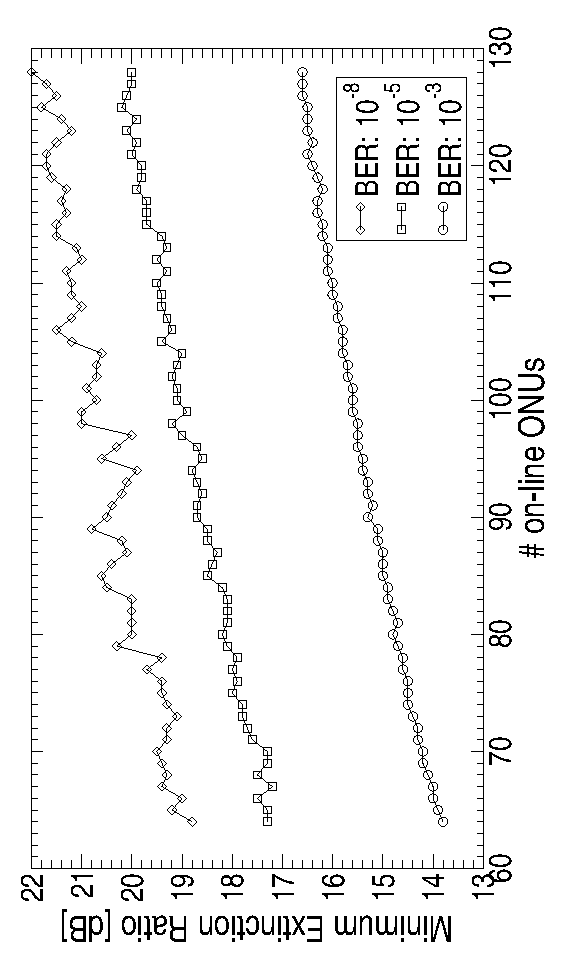
\includegraphics[angle= 270, width=6 in]{graphs/orte03.pdf}
%      \caption{Physical layer simulation result: Minimal extinction ratio required to assure a given BER}
      \caption{Resultado de simulaciones de la capa física: razón de extinción mínima requerida para asegurar un cierto BER.}
      \label{sim:optical}
\end{figure}
En el escenario de $128$ ONUs presentes, un BER menor a 10e-3 puede ser logrado utilizando transmisores del tipo comercial con una razón de extinción de $\simeq16.6$~dB.
Este BER es lo suficientemente bajo para permitir rutinas de corrección de errores al nivel del canal lógico, que garanticen la transmisión libre de errores con una utilización acotada de la capacidad total del canal.
%In the $128$ ONUs scenario a  BER$<10^{-3}$ can be achieved using
%commercially available transmitters with an extinction ratio $\simeq16.6$~dB.
%This BER is low enough to allow for logical-channel error-correction routines that guarantee error-free transmission, while still making use of a fair fraction of channel capacity.
% perform correctly and still use a fair fraction of channel capacity.
% Fig.~\ref{sim:optical} shows simulation results for the BER vs OSNR
% for different numbers of ONUs with fixed electrical SNR $\simeq 42$~dB.
% Higher BERs as ONUs number increases due to the higher probability of
% simultaneous bit `1' transmissions (collisions) yielding pulses of
% optical power higher than that of a logical
% `1', generating intersymbol interference. Higher powers generate higher
% currents at Rxs that demand longer times to settle to logical `0' levels after
% filtering. Nevertheless, as
% can be seen in fig.~\ref{sim:optical}, in the worst case scenario (128
% ONUs) the expected OSNR at the EDFA output is enough ($\geq 40$~dB) to
% ensure a BER$<10^{-7}$. In this case simulation shown that the occurrence of
% 15 simultaneously active Tx was a very rare event, so optical power at Rx
% would be $\simeq -15$~dBm, well bellow standard commercial Rx overload
% of $\sim0.5$~dBm (maximum acceptable mean input power for a
% BER$<10^{-12}$).

\begin{figure}[t]
  \centering
  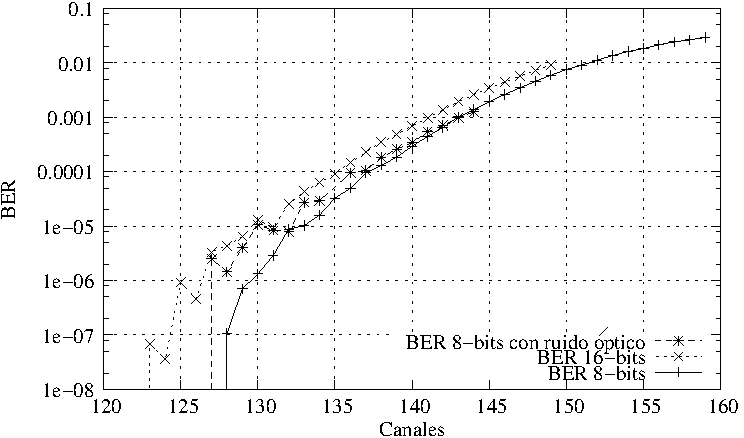
\includegraphics[width=5in]{graphs/BER-tesis.pdf} 
  \caption{BER del canal de un ONU a 10 Gbps vs. la cantidad de ONUs activos. La curva de ``BER 16 bits'' utiliza símbolos de 16-bits. Tiene mejor performance que la curva ``BER 8 bits'' con símbolos de 8 bits. Finalmente, si simulamos el ruido óptico del canal, la performance disminuye ligeramente como puede verse en la curva ``BER 8 bits con ruido óptico''.}
  \label{sim:access}
\end{figure}


La Fig.~\ref{sim:access} muestra los resultados de la simulación del canal, comparando el BER de un ONU con respecto al número total de ONUs activos. Las dos primeras gráficas muestran la diferencia en rendimiento al utilizar símbolos de 8 bits con respecto a símbolos de 16 bits y, en la tercera gráfica se aprecia el aumento en el BER como resultado de agregar una etapa de ruido óptico a la simulación.
Los resultados fueron obtenidos enviando exactamente un gigabit de datos por cada ONU simultáneamente. El mismo método se utilizó para realizar las simulaciones cuyo resultados se presentan en la Fig.~\ref{BERvsExpansion}, donde se observa una mejora de rendimiento importante al utilizar el algoritmo de reducción de peso de Hamming.
Volviendo a la Fig.~\ref{sim:access}, puede verse que cuando la cantidad de ONUs supera los 128, el BER se eleva marcadamente.
De la misma figura podemos observar una disminución de la capacidad en aproximadamente $8$ ONUs cuando el ruido de la capa óptica es agregado a la simulación, debido a la razón de extinción y el ruido producido por el EDFA y los PDs.
Finalmente, la carga máxima que soporta el sistema con un BER de 10e-8 es del $90\%$, lo que significa que en una red de 128 clientes, pueden transmitir simultáneamente hasta 119 ONUs.


%Fig.~\ref{sim:access} shows simulation results for the fraction of the total
%capacity and the BER of one channel at the coding level (circles) and 
%including physical layer impairments (squares). 

%These results were obtained by
%sending one Gigabit of data for each ONU simultaneously.
%This figure shows a channel utilization of $15.7\%$ when all of $128$ ONUs
%are transmitting simultaneously, with a BER$<10^{-8}$. 
%From Fig. \ref{arch:fig1} we observe a penalty of $8$ ONUs when
%impairments from the optical layer (mainly extinction ratio and noise from EDFA and PDs) are taken into account.
%Considering that the system was designed to support asynchronous communications (e.g., Ethernet), it is not likely that all the ONUs will transmit simultaneously (e.g., Internet links often operate at most at $90\%$ load); and therefore our system has a BER $<10^{-8}$ for each channel when 119 ONUs are transmitting at a same time ($119/128>0.9$).
%, removing only one ONU re-establish the desired BER. 
%
%It is worth to remark that, even if the optical channel can induce a
%significant number of errors, the access layer has shown to be able to correct a
%very large number of errors (it is based on
%LDPC+Reed-Solomon+Bloom-Filters), as can be seen on the curve with squares
%at fig.~\ref{sim:access}.
%Observe that the high error rates correspond to a
%worst-case scenario when all ONUs are transmitting simultaneously at
%full capacity, and also 
%there is a low penalty due to physical layer impairments.
%Figure~\ref{sim:optical} presents the simulation's BER vs optical OSNR
%for different numbers of ONUs. %[VAB]
%As the number of ONUs increases higher BERs are obtained at the same optical SNR (electrical SNR is fixed at $\simeq 42\,dB$). In particular there is a penalty of about $30\;dB$ for 128 ONUs in comparison to 1 ONU. This is expected as a consequence of the higher probability of simultaneous bit `1' transmissions (collisions) yielding pulses (logical `1's) of different powers (sum of the power of each transmitter). Higher powers demand more time to settle post filtering current to logical `0' levels. If the following bit slot is indeed a logical `0' an erroneous determination is more possible with a higher collision probability. Nevertheless it can be inferred from simulation results that optical channel should not add significantly to the BER for the whole link as the estimated optical SNR of $\geq 100\,dB$ even for the worst case scenario with 128 ONUs present.
% \begin{figure}[!t]
%     \center
% %     \subfigure[Optical channel]{
% %      \label{sim:optical}
%       \includegraphics[scale=0.4]{BERvsSNR_6GHz.pdf}
% %    }
% %    \subfigure[Logical channel]{
% %      \label{sim:access}
%       \includegraphics[scale=0.4]{BERvsONUs.pdf}
% %    }
%     \caption{Simulation results}
%       \label{archfig}
% \end{figure}

\section{Implementación en FPGA}
El estudio de PONs plantea el desafío de generar, transmitir y recibir señales de 10 Gbps en el laboratorio. El costo de estos sistemas suele ser muy elevado. Uno de los objetivos de esta tesis es presentar una alternativa de muy bajo costo basada en la generación y trasmisión de señales ópticas utilizando dispositivos del tipo FPGA.

\begin{figure}[t]
  \centering
    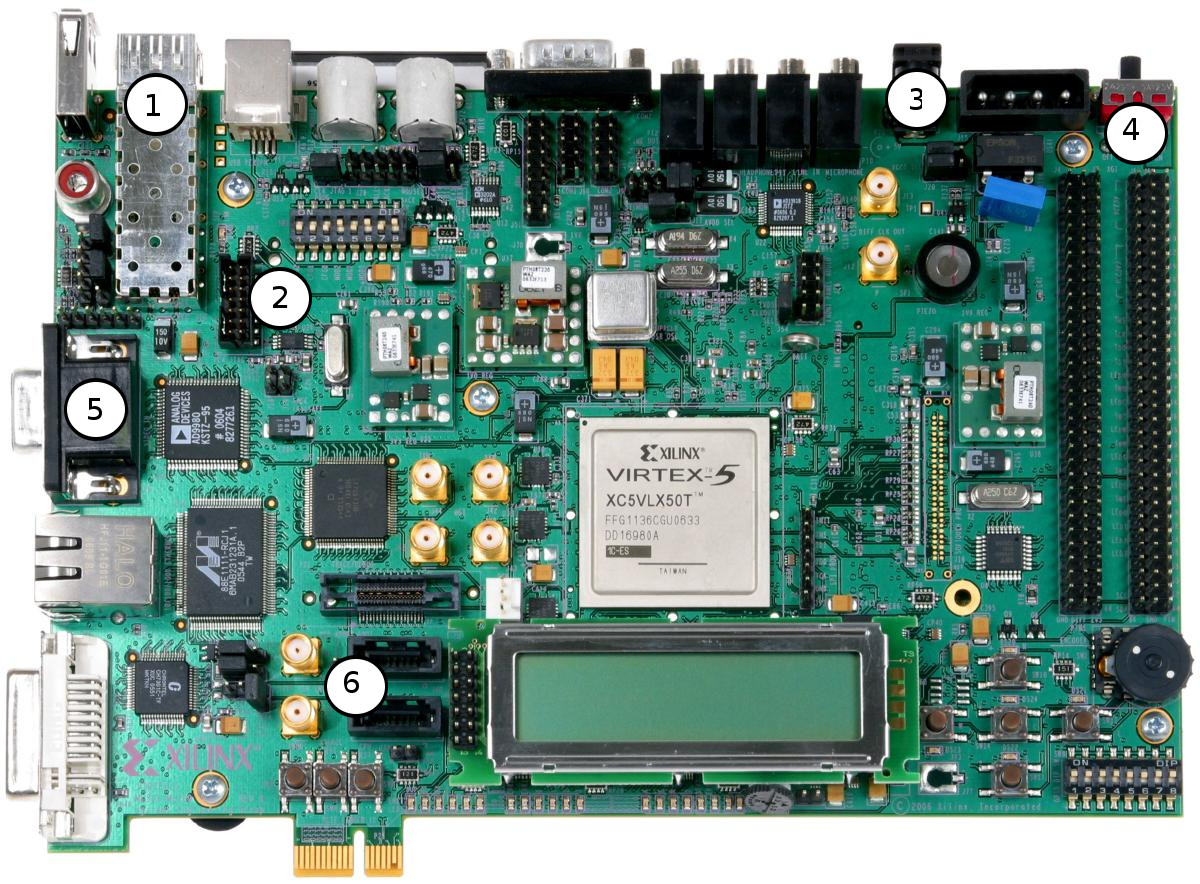
\includegraphics[width=6in]{graphs/ml507.jpg}
\caption {Placa de desarrollo ML570 de Xilinx. Los conectores utilizados son: 1: SFP+, 2: JTAG, 3: alimentación +5V, 4: Switch on/off, 5: Interfaz serial RS232, 6: salida de reloj.}
\label{fig:fpga}
\end{figure}

\subsection{Arquitectura alto nivel de la FPGA Xilinx ML507}
El equipo se compone de un kit de desarrollo ML-507 de Xilinx \cite{virtex5fpga} (ver figura \ref{fig:fpga}) y un transceptor óptico con varios emisores láser con longitudes de onda de 1330 nm y 1550 nm, ambos con capacidad de hasta 10 Gbps en modulación NRZ y alcance de 10km en fibra monomodo \cite{virtex5fpgaRIO}. Para realizar las mediciones se utilizaron dos herramientas de medición:
\begin{itemize}
 \item Osciloscopio óptico Agilent 86100A con módulo óptico 86105A: para
realizar las mediciones físicas contamos con este equipo que posee un
ancho de banda en el módulo óptico de 20 Ghz, suficiente para capturar en
tiempo real los bits individuales o realizar un diagrama de ojo.
\item {\em Integrated Bit Error Rate Tester} (iBERT) \cite{4gtxs}: este dispositivo es un medidor de tasa de error con interfaz para la herramienta de
verificación y depuración ChipScope \cite{arshak2006testing}. Esta herramienta puede denominarse ``virtual'' ya que consiste íntegramente en nucleos IP (\textit{intellectual property}) púramente lógicos, que deben ser sintetizados y embebidos junto con el diseño dentro de la FPGA.
Con iBERT es posible medir en tiempo real varios parámetros del transceptor, así como realizar estadísticas y mediciones de error, variando tasas y características de la transmisión en tiempo real.
 
\end{itemize}
\subsection{Tranceptores multigigabit}
La plataforma de FPGA de Xilinx no fue seleccionada solamente para utilizar la capacidad de procesamiento de la lógica programable para transmisión de datos a altas velocidades, sino por la versatilidad y velocidad de los transceptores multigigabit incluidos en las mismas, esto es, la ``maquinaria'' necesaria para serializar/des-serializar y codificar bits de datos a muy alta velocidad, así como las interfaces para conectar las salidas eléctricas directamente a las entradas de transceptores ópticos, como uno o más SFPs \cite{ug198} (ver figura \ref{fig:fpga}, punto 1). Es necesario mencionar que no existe razón técnica para utilizar un proovedor de FPGAs en particular, ya que muchos proovedores de FPGAs, como por ejemplo Altera \cite{Altera}, venden dispositivos de similares características y precio que Xilinx.

Los transceptores multigigabit están preparados para operar en diversos medios físicos como, por ejemplo, cables trenzados de cobre o líneas de transmisión de alta velocidad sobre PCBs (\textit{printed circuit boards}). Serial-ATA \cite{serial2001high} y PCI-Express \cite{budruk2004pci} son protocolos de transmisión de datos que suelen ser implementados utilizando los transceptores de la FPGA. Sin embargo, en redes de comunicaciones PON, además de funcionar a tasas transmisión  multigigabit se necesitan alcances del orden de kilómetros, características que suelen requerir un medio de transmisión que utiliza fibras ópticas.  El transceptor posee varios módulos adicionales como, por ejemplo, un sistema de sincronización por hardware, sistemas de recuperación de reloj y la capacidad de realizar una codificación 8B/10B \cite{widmer1983dc} adicional, con el objetivo de mantener el balance de DC (\textit{direct current}), pero este último módulo fue desactivado ya que interfiere con los demás codificaciones (para una explicación mas detallada, ver sección \ref{problema8b10b}).

\subsection{Diseño digital del sistema propuesto}
\begin{figure}[t]
  \centering
    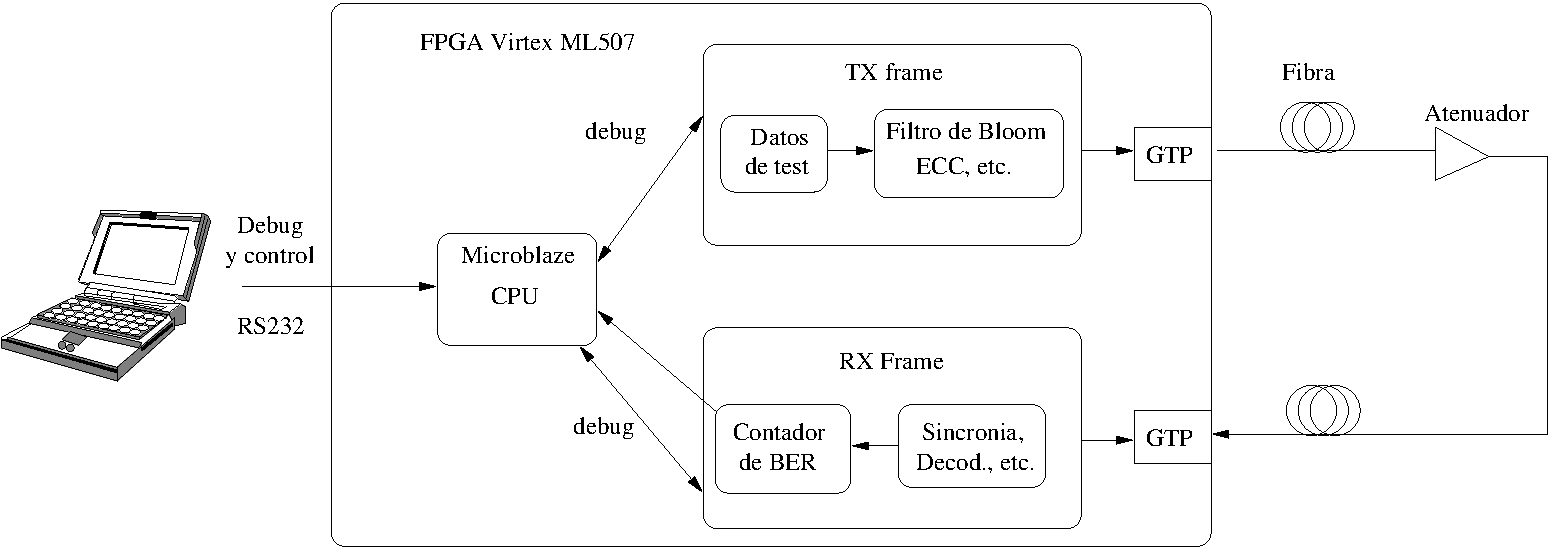
\includegraphics[width=6in]{graphs/fpgadesign.pdf}
\caption {Diseño lógico de alto nivel sobre FPGA}
\label{fig:fpgadesign}
\end{figure}

En la Fig.~\ref{fig:fpgadesign} puede observarse el diseño digital propuesto en el cual se implementó y probó exitosamente el algoritmo transmitiendo a tasas de 5 Gigabits mediante una fibra óptica.
Estas velocidades fueron logradas gracias a ciertas características del diseño que serán descritas a continuación. En la Fig.~\ref{fig:fpgahard} se muestra el diseño digital o de hardware. En esta figura, puede verse que el sistema se compone de dos módulos principales: el CPU que actua de módulo de control y el coprocesador de comunicaciones. El diseño fue realizado íntegramente para la Tesis, y puede manejar tasas de 5 Gbps con un reloj del sistema de sólo 75 Mhz.

El módulo de control cumple la función de interfaz entre el sistema y el usuario, permitiendo modificar parámetros de manera sencilla y presentar las estadísticas de una manera rápida. Se presenta al usuario como un sistema de menús en modo texto, mediante los cuales el operador puede ejecutar comandos y leer valores del sistema. La interfaz al usuario se realiza a través de un puerto serial del tipo RS-232. Para su implementación se utilizó un soft-CPU (CPU sintetizado dentro de la misma FPGA) del tipo Xilinx Microblaze \cite{Xilinx:DS865}, y un programa en lenguaje C encargado de imprimir los menús de control y enviar y recibir datos hacia los módulos generadores y decodificadores de trama. Las operaciones se realizan de manera asincrónica con el resto del hardware, por lo que la velocidad de reloj del CPU puede ser muy reducida. Este módulo se implementa en el archivo ``copro1.v'' que también es el módulo principal del diseño, interconectando las señales de todos los submódulos de generación y decodificación de tramas.


\begin{figure}[t]
  \centering
    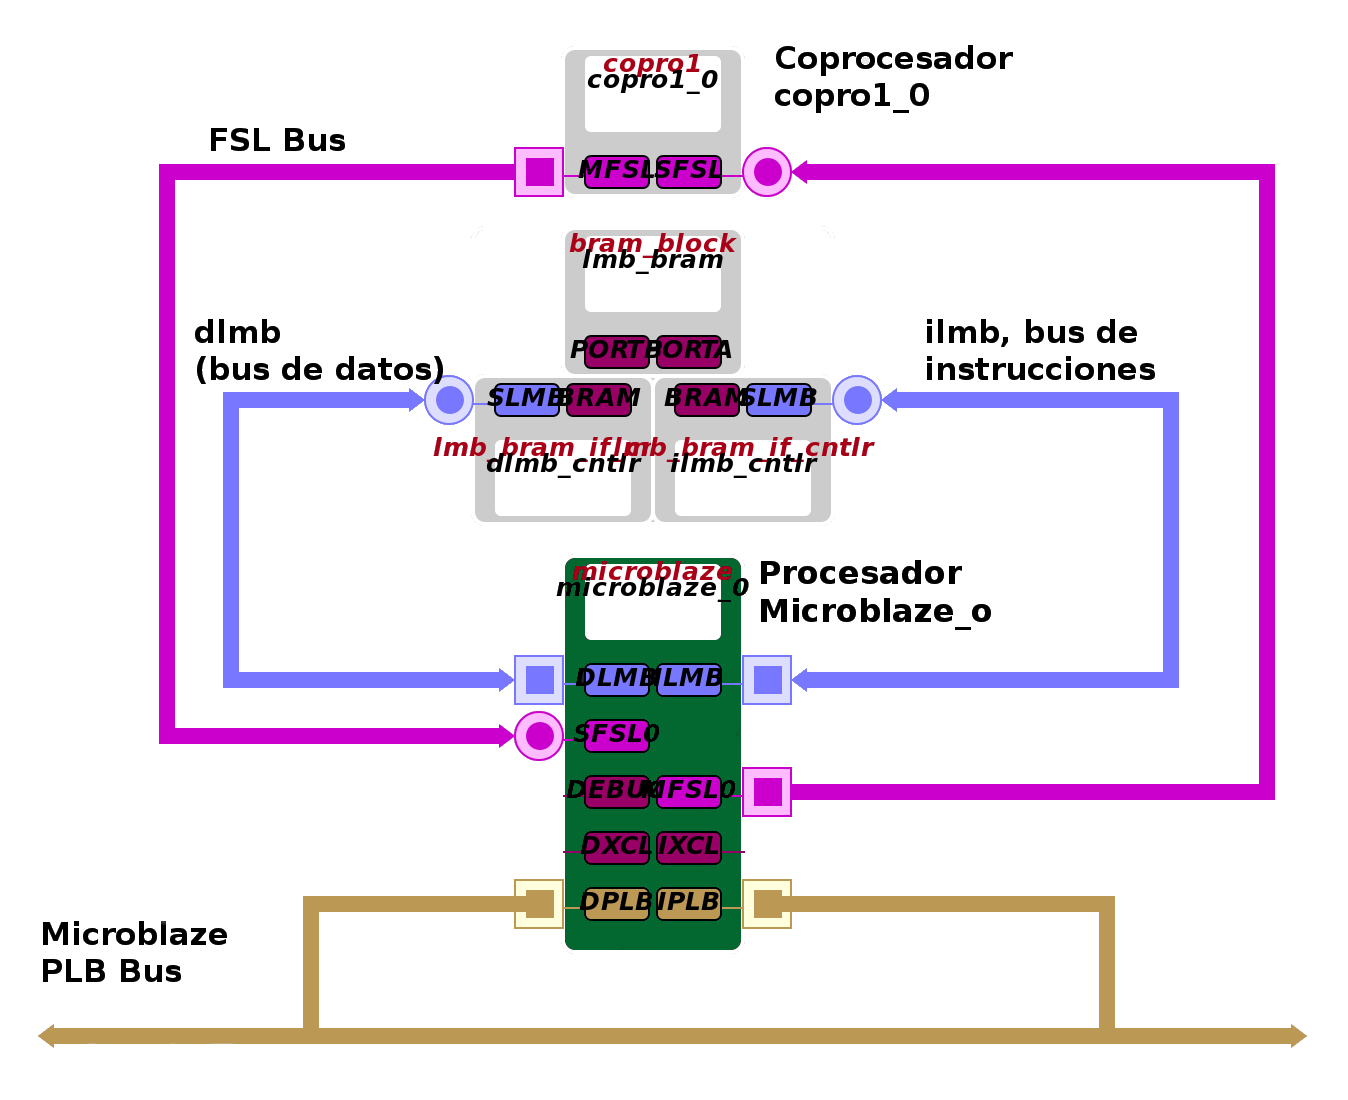
\includegraphics[width=5.25in]{graphs/diagramaXilinx.png}
\caption {Diseño de hardware sobre la FPGA: se aprecian los módulos principales, siendo copro1 el coprocesador de comunicaciones. microblaze\_0 es el CPU y bram\_block es el bloque de memoria utilizado por el CPU, conectado al mismo mediante dos buses: dlmb y ilmb, buses de datos e instrucciones del tipo LMB (\textit{local memory bus}). El coprocesador se conecta mediantes dos buses, llamados copro1\_0\_to\_microblaze\_0 y microblaze\_0\_to\_copro1, ambos buses del tipo FSL (\textit{fast simplex link}). Finalmente, el CPU se conecta a los periféricos como RS232 y switches por medio del bus mb\_plb, del tipo PLB (\textit{peripheral local bus)}.}
\label{fig:fpgahard}
\end{figure}

El coprocesador de comunicaciones puede separarse en cuatro sub-módulos:

\begin{description}
 \item[Transceptor multigigabit:] este componente de hardware es provisto por la FPGA. Puede pensarse en alto nivel como un serializador/deserializador (SERDES), pero contiene más de 15 subsistemas, incluyendo buffers, PLLs (\textit{phase-locked loop}), codificadores y decodificadores. Adicionalmente, el transceptor posee herramientas para sincronización y depuración, permitiendo realizar mediciones y crear lazos de realimentación o \textit{loopbacks} en tres puntos diferentes del flujo de datos para detectar anomalías. Se conecta a la lógica programable de la FPGA por medio de más de 200 señales de control y transferencia de datos, cuyas funciones son encapsuladas por un módulo especial de lógica, que simplifica la interfaz con el resto del sistema. Esta lógica de interfaz se implementó como un módulo de Verilog, llamado ``v5\_gtxwizard\_v1\_7\_tile.v'' en el código fuente.

 \item[Generador de trama:] este módulo se encarga de codificar los datos a transmitir y enviarlos por el transceptor multigigabit. Contiene implementaciones de todas las etapas necesarias, tales como el codificador de ARC4, Bloomfilter encriptado y expansión de peso de Hamming, así como también el sistema de sincronización de trama. La estructura interna es la de una máquina de estados finita, estando implementada íntegramente en lógica digital (sin utilizar ningún componente de software). Se implementó en un sólo módulo de Verilog llamado ``frame\_gen.v''.
 
 \item[Decodificador de trama:] la contrapartida del generador de trama es el decodificador, que posee los decodificadores correspondientes tales como Reed-Solomon, ARC4, Bloomfilter, expansión de peso de Hamming y finalmente el sincronizador de trama, que utiliza parcialmente el hardware de sincronización del transceptor multigigabit para ajustar los tiempos de recepción a nivel de byte, sumado a una sincronización propia para lograr ajustes a nivel de double-word y finalmente, sincronización de la trama (ver sección \ref{fpga:sync}). En lugar de un diseño convencional del tipo CPU+memoria, el diseño de este módulo consiste en una máquina de estados finitos implementada puramente utilizando elementos lógicos de la FPGA. Se implementó en un sólo módulo de Verilog llamado ``frame\_dec.v''. Adicionalmente, un contador de BER se implementó en esta fase, dado que los datos enviados son un patrón de prueba y es posible medir la tasa de errores de manera simple. Las estadísticas de errores son exportadas mediante señales conectadas al módulo de control.
 
 \end{description}

 

El sistema utiliza buffers tanto de lectura como de escritura al transceptor, por lo que puede operar a velocidades de reloj mucho menores. Por ejemplo, si el transceptor multigigabit posee un ancho máximo de bus TXDATAWIDTH y la velocidad de transferencia es TXCLOCK, la velocidad de reloj DATACLOCK necesaria para mantener los buffers internos del transceptor llenos es simplemente $DATACLOCK=TXCLOCK/TXDATAWIDTH$, por lo que transmitiendo a 5 Gbps utilizando el máximo TXDATAWIDTH de 32 bits, tenemos que $DATACLOCK=156Mhz$ un valor alcanzable para la FPGA utilizada y fácilmente implementable en un futuro diseño de ASIC (\textit{application-specific integrated circuit}).
La velocidad de las implementaciones de generador CSPRNG ARC4 y el codificador/decodificador de Reed-Solomon son críticas para la performance del sistema ya que el resto de las etapas no introducen mayores retrasos. El algoritmo ARC4 fue implementado en Verilog poniendo especial énfasis en la performance, logrando un flujo de salida de un byte pseudoaleatorio por cada ciclo de reloj. Para el algoritmo Reed-Solomon se utilizó un IP de la biblioteca de Xilinx que tiene una performance óptima. Exceptuando este último algoritmo de Reed-Solomon, todo el resto del sistema fue implementado desde cero.

% de confEUA.tex

\subsection{Transmisión a 9 Gbps con SFP+}

\begin{figure}[!t]
   \centering
   \subfloat[Tasa de $4.5$ Gbps, 50ns por división.]{{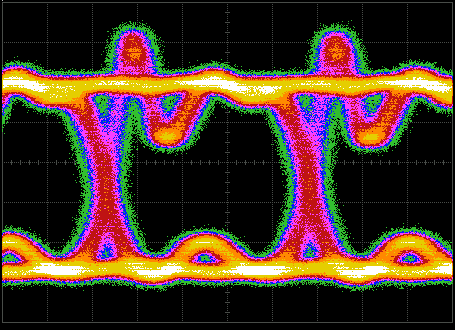
\includegraphics[width=0.45 \textwidth]{graphs/medicionesPaper/eye45G.png} }}%
   \qquad
   \subfloat[Tasa de $7.5$ Gbps, 20ns por división.]{{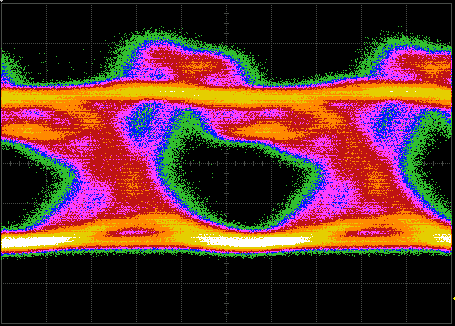
\includegraphics[width=0.45 \textwidth]{graphs/medicionesPaper/eye71G.png} }}%
   \qquad
  \caption {Diagramas de ojo de la señal óptica a la salida de la fibra. Se observa una degradación importante de la calidad de la señal al aumentar la tasa de bits.}
  \label{fig:ImgOjo}
\end{figure}


La norma SFP+ \cite{sff4sff} (\textit{enhanced small form-factor pluggable}) especifica las dimensiones físicas y conectores eléctricos del transceptor óptico. Permite velocidades de hasta 16 Gbit/s y es el formato de transceptor utilizado en la mayoría de los kits de desarrollo de FPGA comerciales actuales.
El transceptor SFP+ consta básicamente de un emisor láser, un detector y circutos ser-des (serializadores/deserializadores).
El montaje para la experiencia se realizó conectando un transceptor SFP+ (ver figura \ref{fig:fpga}, punto 1) con un láser de 1550 nm 
al conector correspondiente en la placa de desarrollo ML-507 y un bucle de
fibra óptica ({\em loopback}), con el objetivo de realizar las mediciones de BER. Adicionalmente, generamos el disparo del
osciloscopio mediante la señal eléctrica de reloj del sistema que
se obtiene a través de los conectores SMA con código J12 y J13 (ver figura \ref{fig:fpga}, punto 6).  
Al disparar el osciloscopio con la señal de reloj sincronizada con la señal de salida, podemos obtener el diagrama de ojo de la señal (ver figura \ref{fig:ImgOjo}).

Para la depuración y configuración se utilizó la interfaz JTAG USB de Xilinx ``Platform Cable
USB II'' \cite{XilJtag} (ver figura \ref{fig:fpga}, punto 2).


\subsection{Configuración del reloj del transceptor}

La tasa de transmisión del transceptor GTX está dada por la
frecuencia de reloj de entrada $F_{PLL\_Clock}$, donde se transmite un
bit por cada semiciclo (la modulación es NRZ); entonces, la tasa de
transmisión será
$R_{line}\mbox{[bps]}=F_{PLL\_Clock}\mbox{[$\frac{1}{s}$]} \times 2$.  La
frecuencia del reloj de entrada del PLL está especificada por la ecuación
5-1 \cite{ug198}:

\begin{equation}
F_{PLL\_Clock} = F_{CLKIN} \times \frac{PLL\_DIVSEL\_FB \times
DIV}{PLL\_DIVSEL\_REF}.% \enspace
\end{equation}\\

donde las constantes $PLL\_DIVSEL\_REF = \{1;2\}$, $DIV = \{4;5\} $ y

$PLL\_DIVSEL\_FB = \{1;2;3;4;5\}$ son configurables por software;
y la frecuencia base del PLL se configura con el switch físico
SW6~\cite[Tabla 1-32]{ug347}.


 Modificando los parámetros puede lograrse, en teoría, un amplio rango
de frecuencias $F_{PLL\_Clock}$, pero de acuerdo a la documentación
del PLL \cite[Pág. 71]{ug366}, este tiene un rango de operación nominal desde $1.2$ a
$2.7$ Ghz. Sin embargo, es posible \cite{OBGAH2010} la
obtención y medición de velocidades de oscilación estables para el PLL
de hasta $4.5$ Ghz (lo que implica una tasa de transmisión de $9$ Gbps),
fuera del rango de operación especificado por el fabricante.

\begin{figure}[t]
  \centering
    %\includegraphics[scale=0.70]{plot.png}
    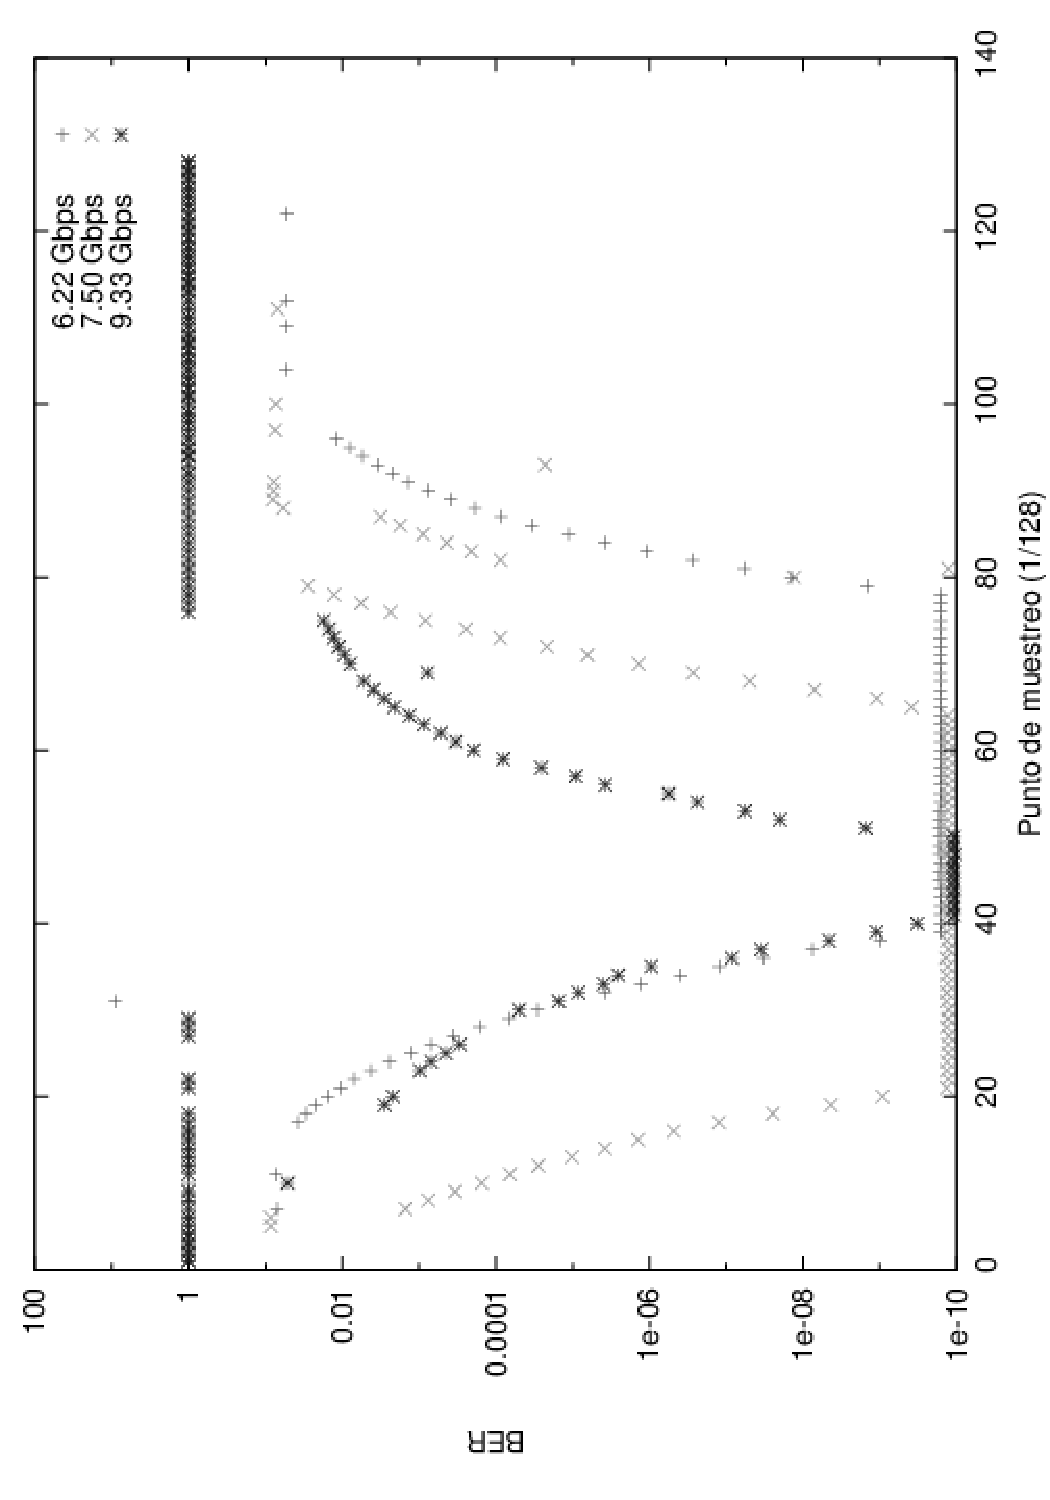
\includegraphics[width=4.2in,angle=270]{graphs/BER_sp_gray.pdf}
\caption {BER vs. punto de muestreo: la FPGA permite muestrear el valor del bit en 128 puntos equidistantes dentro del tiempo de bit. El BER aumenta cuando el punto de muestreo esta cerca de los extremos del bit (valores 0 y 128), donde el diagrama de ojo es más cerrado. Los diagramas de ojo pueden verse en la Fig. \ref{fig:ImgOjo}.}
\label{fig:BERvsSamplingPoint}
\end{figure}

\subsection{Características del transceptor multigigabit a altas velocidades}


\begin{figure}[!t]
   \centering
   \subfloat[Señal óptica a $4.5$ Gbps]{{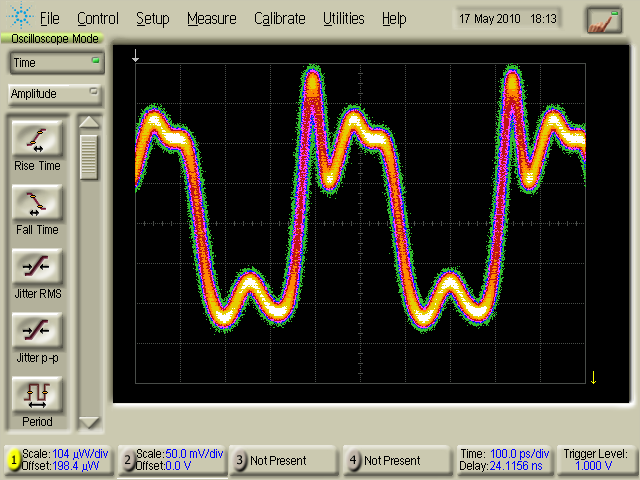
\includegraphics[width=0.40 \textwidth]{graphs/medicionesPaper/screen3.png} }}%
   \qquad
   \subfloat[Señal óptica a $6$ Gbps]{{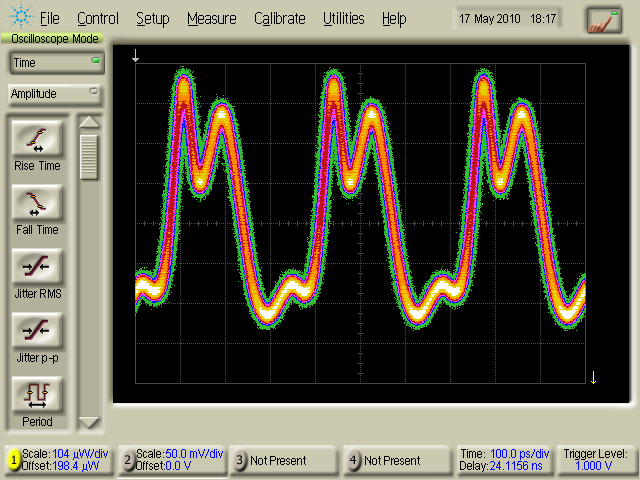
\includegraphics[width=0.40 \textwidth]{graphs/medicionesPaper/screen4.png} }}%
   \qquad
   \subfloat[Señal óptica a $7.5$ Gbps]{{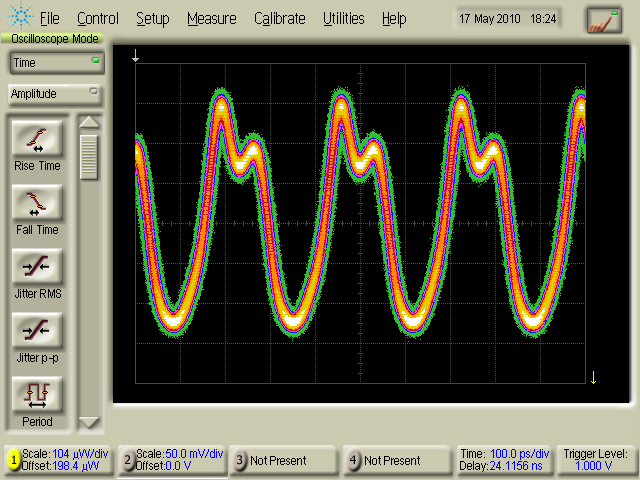
\includegraphics[width=0.40 \textwidth]{graphs/medicionesPaper/screen5.png} }}%
   \qquad
   \subfloat[Señal óptica a $9.33$ Gbps]{{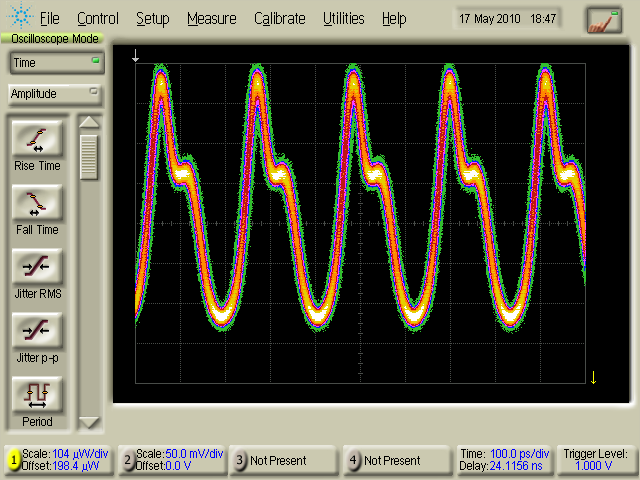
\includegraphics[width=0.40 \textwidth]{graphs/medicionesPaper/screen6.png} }}%
   \qquad
   \subfloat[Señal óptica a $12.44$ Gbps]{{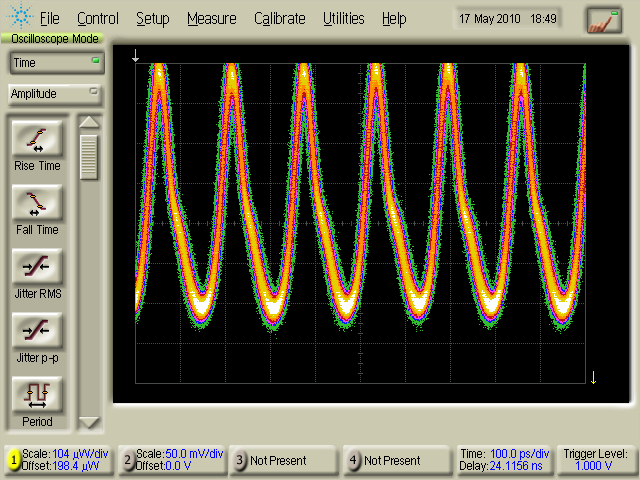
\includegraphics[width=0.40 \textwidth]{graphs/medicionesPaper/screen7.png} }}%
   \qquad
   \subfloat[Señal óptica a $12.44$ Gbps, transmisión 10110101010]{{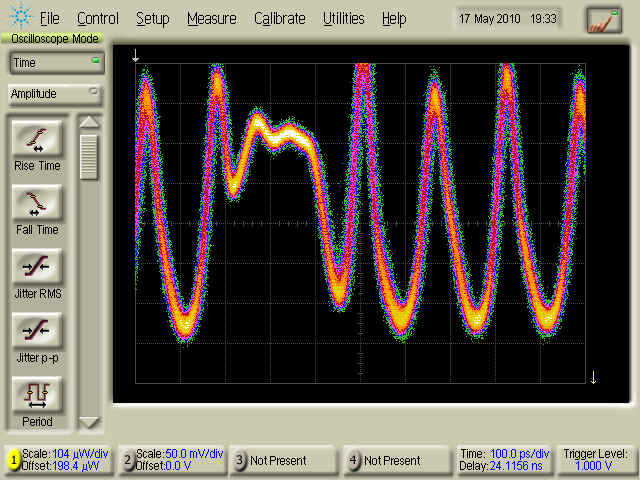
\includegraphics[width=0.40 \textwidth]{graphs/medicionesPaper/screen12.png} }}%
  \caption {Medición de la señal óptica variando la tasa de transmisión de $4.5$ Gbps a $12.44$ Gbps. Se debe tener en cuenta que la señal será distorsionada debido al ancho de banda máximo del módulo de entrada óptico del osciloscopio, que es de 20 Ghz. La secuencia de bits enviada en todas las figuras es ``1010101010'' excepto en la figura f, donde es ``10110101010''.}
  \label{fig:ImgTasa}
\end{figure}





La Fig.~\ref{fig:ImgTasa} muestra la evolución de la señal óptica producida a diferentes
tasas. Según la documentación del tranceptor \cite{ug198}, la máxima velocidad de transmisión es de $6.5$ Gbps. Sin embargo, en la figura se observan mediciones a tasas mucho mayores, de hasta $12.44$ Gbps. Esto obedece a dos razones:
\begin{itemize}
 \item Es posible transmitir y recibir datos hasta una tasa de 9.33 Gbps, si en lugar de utilizar el procesador de la FPGA para realizar las mediciones, se utiliza el contador interno del transceptor. Esto es, los datos no son generados ni contabilizados por la FPGA, sino por circuitos de testeo dentro del mismo tranceptor, por lo que es posible alcanzar tasas mayores.
 \item Si eliminamos la necesidad de recibir y contabilizar los datos, el transceptor puede generar señales de hasta $12.44$ Gbps. A estas tasas el transceptor sólo puede ser utilizado como un generador de señales, ya que no es posible realizar mediciones de BER. Un estudio más detallado de estos métodos puede verse en \cite{OBGAH2010}.
\end{itemize}


Todas las señales en la Fig. ~\ref{fig:ImgTasa} corresponden a una transmisión de la secuencia 10101010, excepto la última figura,
que fue generada con una secuencia distinta para demostrar el control sobre la señal generada.

Para determinar el valor del bit, el circuito receptor muestrea la señal de entrada en un punto determinado dentro del casillero o tiempo de bit. Este punto de muestreo de la señal es importante, ya que si se elige correctamente se minimizará el BER, tal como lo muestra la Fig.~\ref{fig:BERvsSamplingPoint}, donde se aprecia como el BER es minimizado si el punto de muestreo se encuentra aproximadamente en la mitad del tiempo de bit. 
Como puede verse en las Figs.~\ref{fig:ImgOjo}, a tasas elevadas el pulso del bit se deforma y el punto de muestreo óptimo se modifica.


\subsection{Problema de línea desbalanceada y codificación 8B/10B}
\label{problemacodificacion}
\begin{figure}[t]
  \centering
    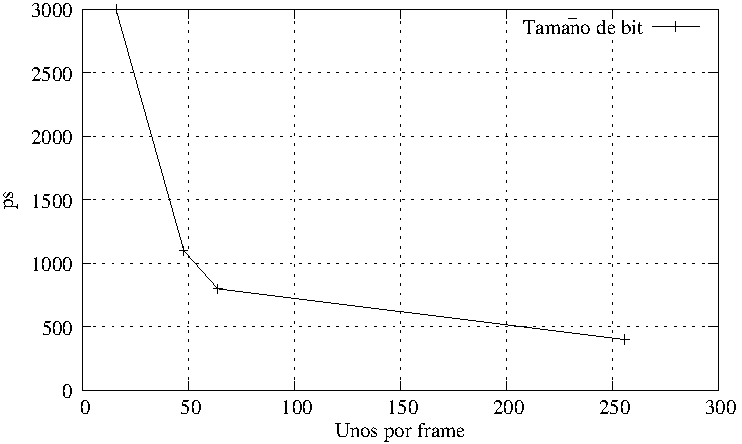
\includegraphics[width=5in]{graphs/expansionbit.pdf}
\caption {Se detalla la expansión del tiempo de bit (en picosegundos) en una señal desbalanceada a medida que la cantidad de unos por trama va disminuyendo. El tamaño de trama es de 512 bits, la tasa nominal es 2.5 Gbps y la duracion del bit es de 400ps.}
\label{fig:expansionbit}
\end{figure}

\label{problema8b10b}
La conexión eléctrica de la FPGA al módulo láser SFP+ se compone de 4 pares diferenciales, que deben transportar señales de hasta 4 GHz. En amplificadores eléctricos de alta velocidad, es deseable que la señal esté balanceada para obtener un componente nulo de corriente continua y poder acotar el ancho de banda necesario. Adicionalmente, una codificación donde se garanticen las transiciones de nivel cada un determinado número de bits, elimina el requerimiento de relojes de alta precisión en ambos lados de la línea de transmisión, ya que el reloj receptor puede re-sincronizarse utilizando dichas transiciones. Esto se logra mediante el denominado circuito de recuperación de reloj.
Uno de estos algoritmos de balanceo es el denominado 8B/10B aunque existen otras codificaciones mas complejas. El transceptor multigigabit de Xilinx tiene un módulo de hardware interno que soporta codificación y decodificación 8B/10B automática de los datos de salida y entrada.

Sin embargo, esta codificación es incompatible con la implementación del algoritmo diseñado sin realizar modificaciones. Si se elimina esta codificación, la señal se degrada tal como se muestra en la Fig.~\ref{fig:expansionbit}, donde mediante mediciones directas con el osciloscopio óptico se aprecia una expansión progresiva del ancho de bit a medida que el desbalanceo de la señal se hace más pronunciado. Los efectos de la expansión del tamaño de bit son evidentes en la fig.~\ref{fig:ImgExpansion} donde las gráficas de potencia óptica ponen en evidencia la expansión e interferencia causada por una señal desbalanceada.
Efectivamente, el receptor recibe hasta 3 ``unos'' por cada ``uno'' transmitido de manera desbalanceada, generando una interferencia que impide el funcionamiento del sistema.


\begin{figure}[!t]
   \centering
   \subfloat[Señal con 256 bits en uno por trama (8B/10B), 400 ps por bit]{{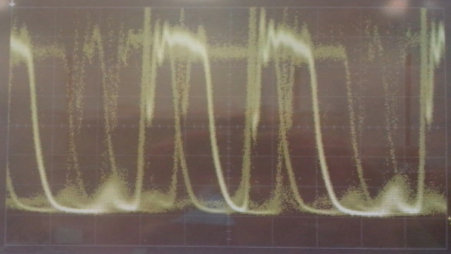
\includegraphics[width=0.45 \textwidth]{graphs/expansion1.jpg} }}%
   \qquad
   \subfloat[Señal con 48 bits en uno por trama, 1100 ps por bit]{{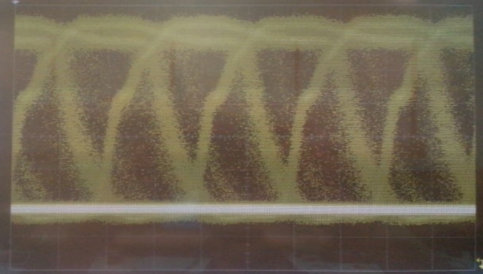
\includegraphics[width=0.45 \textwidth]{graphs/expansion2.jpg} }}%
   \qquad
  \caption {Señal de potencia óptica de un Láser SPF+ Sumitomo de 1330 nm. Se observa una expansión de bit cuando se reduce la cantidad de unos por trama, desbalanceando la señal. La tasa nominal utilizada para estas mediciones es de 2.5 Gbps}
  \label{fig:ImgExpansion}
\end{figure}

Este desbalanceo se soluciona simplemente aplicando las codificaciones a los datos antes de transmitirlos, tales como 8B/10B. Sin embargo, esta transformación es incompatible con el filtro de Bloom, ya que la interferencia de dos señales basta para eliminar la codificación y desbalancear nuevamente la señal. Una posible solución sería utilizar un circuito de transmisión eléctrico compatible con señales desbalanceadas. Para el prototipo se utilizó otra solución, con el objetivo de utilizar la placa ML507 sin modificaciones y poder realizar mediciones sobre el protocolo: en el prototipo, uno de los clientes transmite su señal encriptada normalmente, mientras que los demás clientes son simulados mediante un patrón aleatorio pero balanceado eléctricamente, por lo que la señal es transmitida y recibida correctamente. La señal de estos clientes simulados no puede recuperarse, pero las mediciones son solamente realizadas sobre el cliente real, por lo que el sistema puede funcionar a la máxima tasa soportada por la FPGA (hasta 5 Gbps). El cliente real, al no estar codificado como 8B/10B, introduce un pequeño desbalanceo eléctrico que la línea de transmisión es capaz de soportar sin inconvenientes.

\subsection{Sincronización a nivel de bit, word y trama}
\label{fpga:sync}
\begin{figure}[t]
  \centering
    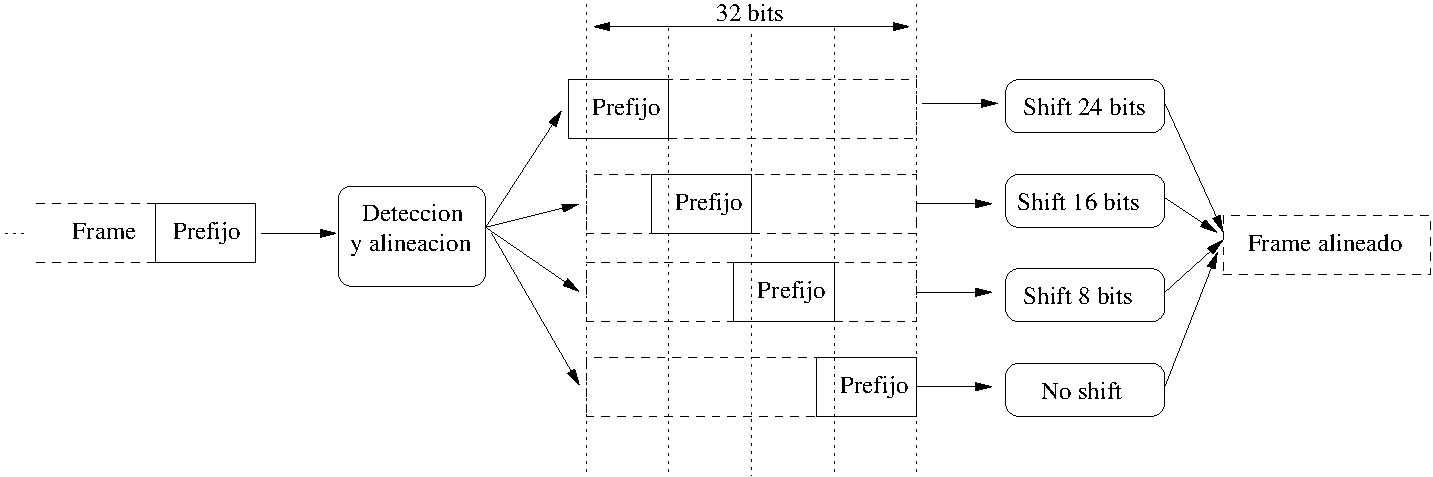
\includegraphics[width=6.2in]{graphs/optsync.pdf}
\caption {Flujo de datos en la sincronización óptica. El mecanismo de sincronización consta de dos etapas: en la primera etapa, el circuito de sincronización de bit alinea la señal entrante al buffer de entrada, colocando el prefijo de sincronización en cuatro posibles alineaciones distintas. La segunda etapa realiza una segunda alineación, detectando la posición del prefijo y utilizando desplazamientos o \textit{shifts} para llevarlo siempre al comienzo del buffer.}
\label{fig:optsync}
\end{figure}


La sincronización no se trató detenidamente en la sección teórica de esta Tesis ya que desde un principio se consideró como un tema ajeno a la misma. Sin embargo, para la implementación final es imprescindible obtener la sincronización entre los nodos que deseen utilizar un canal. Esto no es una tarea sencilla considerando que debe hacerse sobre un canal que contiene una baja relación señal-ruido.

La estrategia utilizada para la transmisión por el medio óptico es utilizar el hardware de sincronización que posee el transceptor multigigabit ya incluido en la FPGA. Este módulo \cite{ug198} denominado ``\textit{Comma Alignment and Detection}'' se basa en la utilización de un prefijo o coma configurable que se compone de una serie de bits (que pueden tener 14 o 20 bits de largo en transceptores de tipo GTX) que se transmite cada vez que se desea sincronizar la etapa RX (receptor) con la TX (transmisor). Esta serie de bits es configurable pero es deseable que posea ciertas características, tales como una alta autocorrelación, para optimizar su detección en el flujo de datos recibidos.
La sincronización se realiza en dos etapas:
\begin{enumerate}
 \item El cliente que desea establecer un canal seguro envía al principio de sus datos el prefijo de sincronización o \textit{comma} (14 bits). Este prefijo es detectado por el módulo de alineación del receptor, que lo coloca en el buffer de entrada. Sin embargo, no se garantiza que el prefijo este siempre al principio del buffer, sino que puede estar tanto en el bit 0 (que sería una alineación perfecta), como en el bit 8, 16 o 24 (Ver fig.\ref{fig:optsync}). Esto es debido a que este buffer es de tipo anillo (\textit{ring buffer}).
 \item Una vez alineado el prefijo en el buffer de entrada, se detecta en qué posición ha quedado y comenzar a leer la trama desde la posición siguiente. Esto se realiza en el código Verilog sintetizando cuatro detectores que simultáneamente buscan el prefijo en todas las posiciones posibles y deciden en un sólo ciclo de reloj cuál es la alineación correcta. Al haber sólo 4 posiciones, es un algoritmo eficiente.
\end{enumerate}

En teoría, sólo debería realizarse la sincronización al principio de las comunicaciones. En la práctica, los relojes no son perfectos y es necesario sincronizarlos periódicamente. En la implementación óptica, se envía el prefijo de sincronización al comienzo de cada trama.
Para evitar colisiones, el hardware de alineamiento se desactiva al detectarse una buena sincronización y se reactiva al finalizar la recepción de la trama. Esta es una operación extremadamente rápida, ya que al utilizar una tasa de 5Gbps, cada trama de 1024 bits tiene una duración temporal de 200 ns. Es necesario aclarar que este prefijo adicional no es parte del protocolo de seguridad diseñado y fue implementado como parte del prototipo. Su utilización en la versión final revelaría información útil a un posible atacante, como por ejemplo el comienzo de la trama.

\section{Redes acústicas}
\label{redacus}

Las señales de audio o acústicas resultaron ser un medio de transmisión compatible con el sistema propuesto. Las señales acústicas se interfieren típicamente de manera aditiva y un modem acústico suele representarse como un canal binario simétrico en lugar de un canal Z. Sin embargo, al utilizar ciertas modulaciones, tales como OOK (\textit{on-off Keying}) en donde la frecuencia portadora es varias veces mayor al ancho de bit, existen bajas posibilidades de que la interferencia de dos señales sea destructiva (es decir, que una señal de audio anule a la otra), mientras que los ceros se modulan como silencios y no causan interferencia. Esto puede aproximarse como un canal Z mediante el cual puede implementarse el sistema de comunicación segura descripto en esta Tesis. Debido a las características de modulación necesarias, las velocidades de transmisión son muy bajas, ya que la respuesta en frecuencia de un transductor acústico típico, como un parlante o micrófono, es relativamente reducida, de 2 KHz a 15 KHz, por lo que el ancho de banda disponible es mucho menor con respecto a la implementación óptica.
No obstante, las pruebas e implementaciones sobre este medio pueden ser realizadas totalmente vía software, y el sistema puede ser utilizado en muchas aplicaciones que no requieran elevadas tasas de transmisión pero que requiera privacidad en la comunicación. Ejemplos de aplicaciones de este tipo pueden ser:
\begin{itemize}
 \item Aplicaciones bancarias
 \item Autenticación multi-factor
 \item Compartir datos de contacto sin necesidad de conexión de red.
 \item Compartir URLs
\end{itemize}

La viabilidad de este sistema se demuestra con la reciente publicación de aplicaciones que utilizan este mismo método, utilizando ondas sonoras, para compartir fragmentos de información tales como URLs y contactos. Una aplicación popular de este tipo es Google Tone \cite{GoogleTone}, desarrollada por la empresa Google, que funciona como una extensión de su navegador de Internet.

\subsection{Modulación}
% de newJIS_140512
Las técnicas de modulación en medios de transmisión acústicos son las mismas que pueden utilizarse en medios electromagnéticos.
Sin embargo, no todas las modulaciones siguen el comportamiento de canal Z descripto en la sección \ref{canalZ}.
La modulación OOK (un caso especial de modulación ASK, \textit{amplitude shift keying}), es uno de los tipos de modulación que permite implementar un canal Z sobre un medio acústico si se utiliza sobre cierto rango de parámetros. Utilizando transductores (micrófonos y parlantes) comerciales del tipo presentes en la mayoría de los dispositivos móviles, como por ejemplo teléfonos celulares, la frecuencia de portadora puede variar de 10 kHz a 16 kHz. El mejor rendimiento del sistema se obtuvo con una tasa de transmisión de 1 Kbps al nivel de trama. En las secciones siguientes se detallan las mediciones del retraso (\textit{delay}), el tiempo que le lleva a un bit atravesar la red, que es relativamente elevado debido a una combinación de la baja velocidad de transmisión y la necesidad de un buffer relativamente grande (2048 bits), necesario para la utilización del esquema de corrección de errores seleccionado (Reed-Solomon 223/255). Si bien aumentar la velocidad de transmisión requiere un esfuerzo considerable debido al bajo ancho de banda disponible, la modificación del algoritmo de corrección de errores o sus parámetros (por ejemplo, utilizar algún esquema tipo BCH \cite{bose1960class}) podría reducir el retraso de datos de manera considerable.

Para acotar el ancho de banda de la señal emitida, se utilizó la técnica de ``\textit{pulse-shaping}'', implementada como un filtro FIR \cite{oppenheim1989discrete} (\textit{finite impulse response}) pasa banda a la salida de la etapa de modulación, así como también en la entrada de la etapa de demodulación. Este filtro, además de reducir el ancho de banda utilizado, ayuda a rechazar interferencias.
Adicionalmente, un ciclo de trabajo (\textit{duty cycle}) de 50\% demostró ser el óptimo para la modulación.
%On-Off Keying modulation of sound waves, following the Z-channel interface model described in Section 2.2., encode the transmitted bits as pulses. Carrier frequency can vary from 10 kHz to 16 kHz. Good results can be obtained with a rate of 1000 bps at frame level. In experiments, delay (the time for a bit to traverse the network) was very high, due to Reed-Solomon 223/255 coding, a frame to support up to 16 users and the low capacity of the physical media. A more sensible choice of FEC algorithm (like BCH [12]) could drastically reduce data delay. 

%Simple pulse shaping is realized using a pass-band filter at the output of the modulation and also at the input of the demodulator. This filter also helps reject unwanted interference.
\subsection{Sincronización}
% de newJIS_140512

\begin{figure}[t]
  \centering
    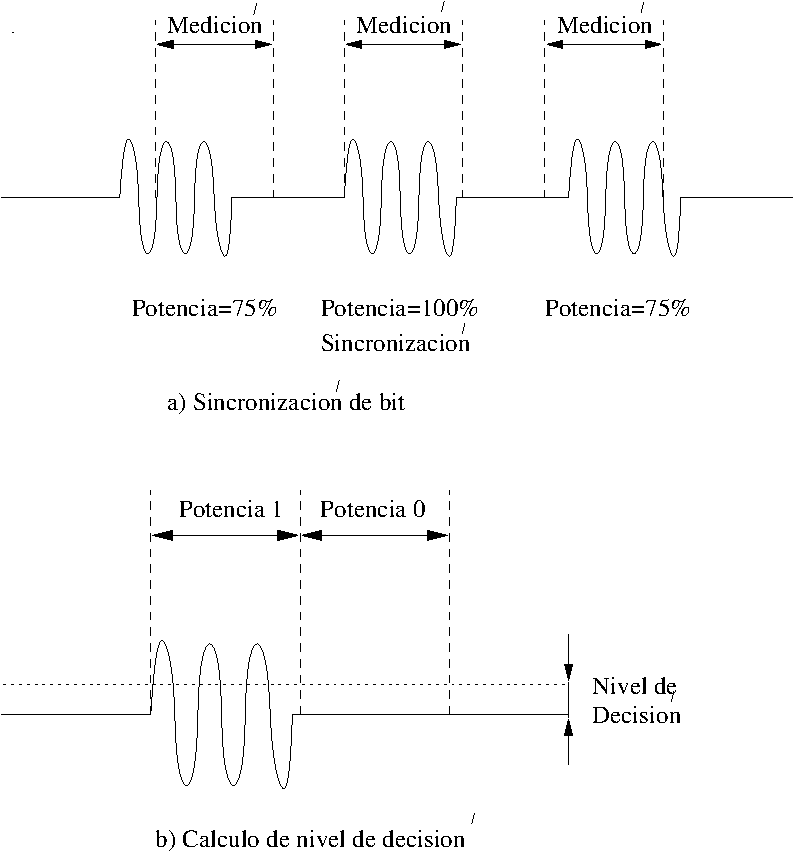
\includegraphics[width=4.5in]{graphs/acusync.pdf}
\caption {Sincronización acústica. En la figura a) se recorren consecutivamente todas las posibilidades hasta encontrar la mayor potencia de bit, que corresponde a la mejor sincronización. Luego, en la figura b) se calcula el umbral de decisión.}
\label{fig:acusync}
\end{figure}

Como se desprende de la descripción del canal de comunicaciones, la sincronización entre el transmisor y el receptor es esencial para la correcta decodificación de la información. 
En el caso del medio óptico, la sincronización de bit y word (16 bits) debe realizarse a tasas tan elevadas que requiere necesariamente soporte de hardware por parte del transceptor.
Sin embargo, las tasas de transmisión de 1 kbps utilizadas en el canal acústico permiten realizar una sincronización por software sin ningún soporte de hardware adicional, al ser una velocidad manejable por cualquier procesador moderno.
El método es muy similar al utilizado en el canal óptico: un patrón inicial de sincronización es enviado para que el receptor pueda realizar un ajuste de parámetros tales como fase y umbral de decisión (ver Fig.~\ref{fig:acusync}). La deriva y fluctuación del reloj del sistema (\textit{drift y jitter}) no son significativas a esta baja velocidad de transmisión, por lo que no se requiere corrección de ningún tipo, haciendo que la implementación del modem por software sea muy sencilla.
Ciertos parámetros, si bien son inicializados en la etapa de sincronización, son por naturaleza dinámicos y se ajustan periódicamente, como por ejemplo el umbral de decisión, que es recalculado a partir de un promedio de los datos de entrada. La fase es también corregida utilizando los datos de entrada como referencia. Este método de sincronización permite detectar el comienzo de la trama a su vez que se ajusta a nivel de bit; ambas alineaciones son necesarias en cada comunicación (pero la alineación de la trama solamente entre los ONUs comunicantes). Adicionalmente, una vez comenzada la transmisión, los datos serán indescifrables gracias al algoritmo CDMA de \textit{time-hopping} guiado por un CS-PRNG.

%As it follows from the description of the communication channel, synchronization between the transmitter and receiver is essential for the correct decoding of information. For this purpose, an initial synchronization pattern is sent, so the receiver can adjust parameters like phase and decision level (see Figure 3). For the data bits transmission a duty cycle of 50\% showed in our experiments an enhanced detection. Clock drift and jitter are not significant at this low transmission speed and so no correction is required, making the software modem implementation very simple. Decision level is dynamic, meaning it is constantly re-calculated from averaged input data. The receiver symbol phase is also corrected using the input data as reference. Notice that this simple synchronization method allows detecting the frame start as well as the bit slot; both are needed at every communication. Moreover, once the data began to be transmitted, the communication becomes indecipherable thanks to the CS-PRNG.


\subsection{Medición multiusuario}
\begin{figure}[t]
  \centering
    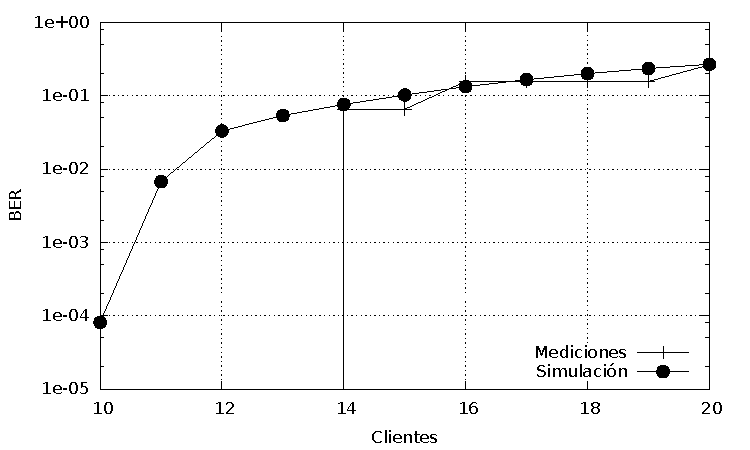
\includegraphics[width=5in]{graphs/medidas_clientes_JIS-fig6.pdf}
\caption {Multi-usuario: BER del enlace entre dos laptops (Lenovo T420 y Lenovo X60), una de ellas simulando varios nodos.}
\label{fig:acumult}
\end{figure}

Todas las mediciones fueron realizadas a una tasa de 1 kbps, utilizando una señal portadora acústica de 16 kHz, que se encuentra en el límite auditivo de la mayoría de las personas adultas \cite{gordon2005hearing}. Es posible que algunos parlantes no respondan correctamente a esta frecuencia, en cuyo caso puede reducirse y utilizar una portadora de 12 kHz. El objetivo de utilizar una frecuencia de audio tan cercana al límite de reproducción de los transductores es incrementar el nivel de confort de los usuarios, que sólo podrán percibir el modem con bajo volumen, o directamente será inaudible. Adicionalmente, las altas frecuencias presentaron menos interferencias de ruido ambiente.
La cantidad total de datos transmitidos por canal fue de 4096 bits en cada medición. El volumen de la señal de salida fue configurado al máximo para cada dispositivo, mientras que la amplificación de la señal obtenida por el micrófono fue optimizada en cada caso para obtener el menor BER.
Con el modulador y circuito de sincronización implementados, el sistema opera con tasas de error aceptables con una separación máxima entre nodos de 1 metro, una distancia que normalmente excede la existente entre un terminal móvil (celular, etc.) y una computadora fija en el mismo escritorio (Ver Fig.~\ref{fig:acudist}). Aún para un alto número de clientes simultáneos ($> 10$) el sistema no presenta altas tasas de error o ancho de banda reducido, como puede verse en la Fig.~\ref{fig:acumult}.
En las mediciones, el retraso del canal fue de más de 60 segundos, excesivo para muchas aplicaciones que no necesitan alto ancho de banda pero requieren un corto tiempo de respuesta (por ejemplo, aplicaciones bancarias). El retraso puede ser disminuido de dos maneras: 
\begin{enumerate}
 \item Decrementando la cantidad máxima de clientes simultáneos soportados por el sistema.
 \item Utilizando algoritmos de ECC de bajo retraso y de bloque reducido, tales como BCH, ya que actualmente el retraso se produce en su mayor parte durante la recepción de un bloque completo para el algoritmo de Reed-Solomon (2048 bits).
\end{enumerate}



% De JIS2014MathType.pdf
%All measurements were conducted at a rate of 1000 bps, with the carrier signal at 16 kHz. The total data trans-
%mitted was 4096 bits. Output volume was set at the maximum possible for each device, while the input amplifi-
%cation was optimized for each measurement.
%We measured that the system operates with acceptable error rates for links of up to 1 meter, a distance usually
%exceeding that between a mobile terminal (phone, etc.) and a fixed computer placed in the same desk (see Fig-
%ure 7). Even for a high number of concurrent clients (>10) the system does not present high error rates or re-
%duced bandwidth, as can be seen in Figure 6.
%Although in the present test channel delay was longer than 60 seconds, excessive for some applications re-
%quiring short response time (e.g. banking transactions), this parameter can be reduced by decreasing the maxi-
%mum number of simultaneous users supported by the system and using a lower-delay interleaver and an outer
%error correction algorithm like BCH
%

\subsection{Mediciónes a distintas distancias}

\begin{figure}[t]
  \centering
    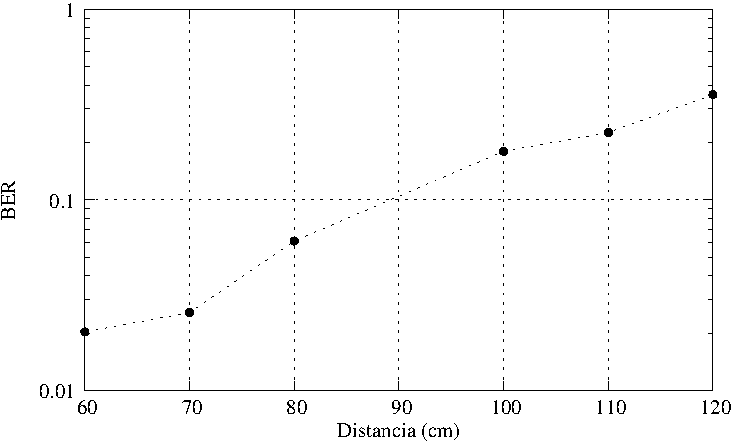
\includegraphics[width=5in]{graphs/mediciones-distancia-fig7.pdf}
\caption {Distancia vs. BER: el enlace acústico entre una Laptop (Lenovo T420) y un celular (HTC Status) presenta errores detectables cuando se superan los 60 cm de separación entre ambos dispositivos.}
\label{fig:acudist}
\end{figure}

Las comunicaciones acústicas utilizando como portadora un tono de 12 kHz son muy susceptibles al ruido ambiente. Un enlace acústico con 50 cm de separación entre una notebook Lenovo T420 y un celular HTC Status (ver Fig. \ref{fig:acudist}) tuvo un $15\%$ de BER con sólo una ligera interferencia (como por ejemplo, golpear una mesa cercana). Esta observación motivó el uso de la frecuencia más alta posible. Una portadora de 16 kHz presentó el mayor rango de compatibilidad entre los dispositivos, aunque algunos de ellos demostraron no poder emitir audio a frecuencias mayores.
Los parlantes de una Laptop Lenovo T420 y otra Laptop Lenovo X60 fueron capaces de establecer un enlace utilizando como portadora un tono de 19.2 kHz, aunque sólo en cortas distancias (20 cm). De todas formas, esta frecuencia de portadora permitió un mayor ancho de banda en el enlace (2 kbps en lugar de 1 kbps) con la misma tasa de error.
%La señal acústica modulada puede causar molestias a personas o animales cercanos. Distintos tonos de portadora causan distintos efectos y niveles de molestia, aunque este último parámetro es subjetivo. La portadora de 19.2 kHz fue descrita como no audible, mientras que la portadora a 16 kHz y 12 kHz son claramente audibles. Se notó que el volumen del sonido modulado y las molestias asociadas al mismo aumentan con el numero de clientes simultáneos transmitiendo en el medio.

% De JIS2014MathType.pdf
%Communications using a 12 kHz tone carrier were extremely susceptible to ambient noise. Indeed, a 50 cm
%link between a laptop Lenovo T420 and a HTC Status phone suffered an excess of 15% BER with slight noise
%%interference (like bumping on a nearby table). This observation motivated the use of the highest attainable fre-
%quency. A 16 kHz carrier provided the widest range of compatibility among tested devices, because some of
%them could not emit at higher frequencies.
%Tests were also done at higher frequencies for capable devices. For instance, laptop speakers in Lenovo T420
%and Lenovo X60 laptops proved capable of establishing a link at 19.2 kHz, but only for very short distances
%(20cm). Nevertheless, this carrier frequency allowed a faster link (2000 bps) with the same BER.
%The modulated sound signal can represent a nuisance to nearby persons and animals. Several different carrier
%frequencies were tested as a way to evaluate the level of discomfort. The 19.2 kHz carrier signal was perceived
%as almost non-audible, with 16 kHz being clearly audible for most people and the link at 12 kHz being the most
%uncomfortable. It should be noticed that loudness and hence discomfort increase with the number of simultane-
%hous users.
%

\chapter{Conclusiones}

En esta Tesis se documentó el diseño un sistema de comunicaciones criptográficamente seguro que aprovecha las técnicas de CDMA sobre fibra óptica y sobre ondas sonoras. Durante el transcurso de la investigación, se desarrolló un algoritmo de corrección de errores asimétrico, optimizado para canales de tipo Z.

El resultado es un sistema de red de tipo difusión, capaz de crear múltiples VLANs criptográficamente seguras utilizando cualquier medio de transmisión que pueda ser modelado como un canal Z. 
Se implementaron simuladores en software con el objetivo de obtener estadísticas y mediciones. Luego se realizaron prototipos funcionales tanto sobre software para el caso del medio acústico, como sobre un dispositivo FPGA en el caso del medio de fibra óptica. El protocolo alcanzó una velocidad de 1000 bps con 16 clientes sobre el medio acústico y 5 Gbps con 128 clientes simultáneos con una separación máxima de 20 km, sobre el medio óptico, con una utilización total del medio del 32\%.

Se mostraron resultados tanto de cálculos teóricos, simulaciónes numéricas y mediciones realizadas sobre los prototipos. Los resultados de los cálculos, simulaciones y mediciones fueron consistentes entre sí.

El esquema de transmisión desarrollado puede utilizarse en cualquier medio de transmisión que pueda representarse como un canal Z, como por ejemplo ondas sonoras o acústicas bajo ciertas modulaciones. Debido a esta característica, el mismo protocolo desarrollado con el objetivo de utilizar fibra óptica como medio de transmisión, fue utilizado en una red acústica de baja velocidad entre dispositivos móviles, con un máximo de 16 dispositivos en la red a una distancia de hasta 1.2 metros. Esto abre las puertas a redes ad hoc privadas entre dispositivos, simplificando aplicaciones que hasta ahora necesitaban de una conexión continua a Internet o de tecnologías del tipo NFC.

Concretamente, se presentó el diseño de una red de difusión con un grado de privacidad criptográficamente fuerte. Para ello se utilizó un filtro de Bloom \cite{Bloom70space/timetrade-offs} encriptado, que es utilizado a la vez como el elemento de cifrado y como una primera etapa de corrección de errores. Adicionalmente, se presentó una codificación de datos novedosa\cite{6476559} que incrementa la eficiencia del filtro de Bloom como algoritmo de corrección de errores. El resultado es un protocolo de VLAN capaz de soportar un volumen de información o \textit{throughput} constante sin importar la carga de la red, manteniendo completa privacidad entre sus nodos.

%asfd_hasta_aca

Se demostró la viabilidad del protocolo mediante la implementacion y medición de dos prototipos: el primer prototipo del sistema de comunicaciónes fue realizado sobre fibra óptica con velocidades de transmisión de 5 Gbps. La plataforma de desarrollo es un transceptor laser de comunicaciones del tipo XFP+, y una FPGA del tipo Xilinx Virtex 5.
El segundo prototipo fue implementado exclusivamente en software y utiliza el mismo protocolo pero con diferentes parámetros, esta vez sobre una red encriptada acústica entre dispositivos móviles sin ningun tipo de modificación o hardware adicional.

Esta Tesis apunta a solucionar uno de los problemas de seguridad mas graves de las redes de difusión, que es la vulnerabilidad a ataques de espionaje. Por ejemplo, un nodo malicioso en un sistema TDMA puede acceder a la información de cualquier otro nodo, tan solo escuchando en el tiempo asignado al nodo víctima, ya que los tiempos de bit son totalmente predecibles.  

En contraste, el sistema presentado en esta Tesis asigna los tiempos de bit de manera pseudoaleatoria, por lo que un nodo malicioso no puede predecir la posición de ningun otro nodo. No existe nigun tipo de arbitraje ni de colaboración entre nodos que pudiera revelar información a un presunto atacante, y se garantiza la comunicación privada de un nodo aún cuando todos los demás nodos del sistema sean maliciosos.

La fuerza criptográfica del sistema esta asociada y es equivalente a la del generador pseudoaleatorio seleccionado para generar los tiempos de bit, siendo el único requerimiento del mismo que sea criptográficamente seguro. Al no existir colaboración y arbitraje entre nodos, la naturaleza o algoritmo de dicho generador puede variar de nodo a nodo sin afectar la performance del sistema. 

La consecuencia de prohibir toda colaboración o arbitraje, es que las colisiones de datos entre nodos son inevitables, y frecuentes. De ahi que el mayor esfuezo de diseño en el del sistema presentado, y el módulo de mayor consumo de recursos computacionales, es la recuperación o corrección de errores, que debe ser suficientemente potente como para reducir las tasas de error a valores utilizables, sin consumir excesivos recursos computacionales o de ancho de banda. El algoritmo final fue medido con un BER menor a 10e-8 con una utilización del medio del 32\%. Otra característica notable es que, al ser los nodos totalmente independientes entre sí, no se produce ningun tipo de degradación de la velocidad o ancho de banda en los canales de transmisión individuales, siempre y cuando la cantidad total de nodos este por debajo del límite diseñado.

\section{Trabajos futuros}

Todos los prototipos realizados son completamente funcionales y cumplen con los objetivos de la Tesis sin embargo, para una implementación comercial a gran escala es posible optimizar ciertos módulos, que serán nombrados a continuación:
\begin{description}
 \item[Codificación] 
El problema de la codificación de línea fue descrito en \ref{problemacodificacion} y una solución aceptable, que permite la creación de un prototipo funcional, fue adoptada. Sin embargo, en una implementación final, se debe contemplar la imposibilidad de utilizar cualquier algoritmo de balanceo ya que no es compatible con el algoritmo de filtro de Bloom. Dado que el problema es de naturaleza eléctrica, es probable que un diseño cuidadoso de los buses entre la FPGA y el transceptor óptico solucione este problema.
 \item[Sincronización] 
 El algoritmo de sincronización es crítico en una implementación real. Las implementaciones realizadas para los prototipos son funcionales pero no son ideales ya que, al utilizar prefijos conocidos, un atacante puede obtener información acerca del comienzo y finalización del frame. La codificación es suficientemente fuerte para que este conocimiento no perjudique el nivel de seguridad, pero es posible el desarrollo de un algoritmo de sincronización criptográficamente seguro, que no revele ninguna información a un posible atacante (ver \cite{jung1999encryption} para un ejemplo de sincronización segura).
 \item[Eliminación del frame] 
 En la sección \ref{Seguridad} se explica que se divide la transmisión en frames, que son segmentos de bits cargados directamente dentro del filtro de Bloom. Esta división en segmentos de los datos no es absolutamente necesaria y podría implementarse una variación del algoritmo que no utilice frames, sino que todas las posiciones de bits sean relativas entre sí, en lugar de relativas al comienzo del frame. Esta variación no incrementa la seguridad pero, probablemente, simplifique la implementación.
 \item[] 
\end{description}


%\chapter{Título Capítulo}
%\chapter{Título Capítulo}

% ********************************************************************
% Backmatter
%*******************************************************
\appendix
\cleardoublepage
%\part{Apéndice}
\chapter{Título Apéndice}



% ------------------------------------------------------------------------

%BIBLIOGRAFIA
\linespread{1.44}
\bibliographystyle{amsplain}
\bibliography{vb_fgct,IEEEabrv,IEEEorte,confEUA}

% =================================================================
% Dummy directive
% Included for Gather Purpose only:
% %input "Xbib.bib"
% is no longer necessary because
%  \bibliography{xbib}
% is now defined as an input directive
% (see Options -> Advanced -> Tree [INPUT_DIRECTIVES] for details...
% It can be reconfigured!
% =================================================================
\end{document}
% ------------------------------------------------------------------------
